
\documentclass[a4paper,12pt,times,numbered,print,index]{report}
\usepackage[english]{babel}
\usepackage[utf8]{inputenc}

\oddsidemargin  0.01mm       % USA 5mm?
\evensidemargin 0.01mm       % USA 5mm?
\headheight -0.03mm             % 10mm ok
\headsep  -0.03mm
\hoffset -3mm
% was commented out before
\textheight 250mm            % USA 240mm?
\textwidth 180mm             % USA 160mm?
\topmargin -10mm           % before 18/5/93 this was -20mm
\topskip -10mm

\renewcommand{\baselinestretch}{1.40}

\renewcommand {\arraystretch}{1.20}


\usepackage{dcolumn}
\usepackage{amsmath}
\usepackage{amssymb}
\usepackage{graphicx}
\usepackage{pdfpages}
\usepackage{fullpage}
\usepackage{caption}
\usepackage{float}
\usepackage{fancyhdr}
\usepackage{amsmath}
\usepackage{multirow}
\usepackage{commath}
\usepackage{natbib}
\setcitestyle{aysep={,}}
%\usepackage{apacite}
%\usepackage{biblatex}
\usepackage{mathtools}
\usepackage{subcaption}
\usepackage{mathrsfs,amssymb}
\usepackage{amsthm}
\usepackage{enumitem}
\usepackage{booktabs}
\usepackage{verbatim}
\usepackage{enumitem,kantlipsum}
\usepackage{chngcntr}
\usepackage{apptools}
\usepackage{adjustbox}
\usepackage{epstopdf}
\usepackage{pdflscape}
\usepackage{afterpage}
\usepackage[pdftex,colorlinks=true,linkcolor=cyan,linktoc=all]{hyperref}
\usepackage{siunitx}
\usepackage{authblk}
\usepackage{soul}

\usepackage{titletoc}% http://ctan.org/pkg/titletoc
\titlecontents*{chapter}% <section-type>
[0pt]% <left>
{}% <above-code>
{\bfseries\chaptername\ \thecontentslabel\quad}% <numbered-entry-format>
{}% <numberless-entry-format>
{\bfseries\hfill\contentspage}% <filler-page-format>


\usepackage[font=footnotesize,labelfont=bf]{caption}
\captionsetup[sub]{font=scriptsize,labelfont=bf}
%\newcommand*{\fullref}[1]{\hyperref[{#1}]{\autoref*{#1} \nameref*{#1}}}

\renewcommand{\sectionautorefname}{Section}
\renewcommand{\subsectionautorefname}{Section}
\renewcommand\thesection{\arabic{section}}

\interfootnotelinepenalty=10000
\setcitestyle{aysep={,}}
\newcolumntype{L}{@{}l@{}}
\newcommand{\mc}[1]{\multicolumn{1}{c}{#1}}
\sisetup{table-space-text-post = **}
\definecolor{darkblue}{rgb}{0,0,.6}
\hypersetup{citecolor=darkblue,linkcolor=darkblue,urlcolor=darkblue}



%\mathchardef\colon="603A
%\appendix{\counterwithin{lemma}{section}}


\makeatletter
%% The "\@seccntformat" command is an auxiliary command
%% (see pp. 26f. of 'The LaTeX Companion,' 2nd. ed.)
\def\@seccntformat#1{\@ifundefined{#1@cntformat}%
	{\csname the#1\endcsname\quad}  % default
	{\csname #1@cntformat\endcsname}% enable individual control
}
\let\oldappendix\appendix %% save current definition of \appendix
\renewcommand\appendix{%
	\oldappendix
	\newcommand{\section@cntformat}{\appendixname~\thesection\quad}
}
\makeatother
\usepackage{cleveref} % just for this example



%\renewcommand{\&}{and}
\numberwithin{equation}{section}
\newtheorem{theorem}{Theorem}[section]
\DeclareMathOperator*{\argmin}{argmin}
\newtheorem{remark}{Remark}[section]
\newtheorem{assumption}{Assumption}
\allowdisplaybreaks
\newtheorem{lemma}{Lemma}

\newcommand{\assumptionautorefname}{Assumption}
\newcommand{\lemmaautorefname}{Lemma}
\newcommand{\qedd}{\tag*{$\qed$}}


\pagestyle{fancy}
\fancyhf{}
\renewcommand{\headrulewidth}{0pt}
%\renewcommand{\headrulewidth}{0.1pt} % for upper line
%\rhead{Weilun Zhou}
%\lhead{Confirmation Report}
\cfoot{\thepage}
%\setlength{\headsep}{0.3in}




\title{{Parametric Single-Index Models: Simulation and Empirical Results} \vspace{2cm}}
\author{Ying Zhou}
\date{March \\ 2021}



\begin{document}
	
	\begin{titlepage}
		\begin{center}
			\vspace*{1cm}
			
			\Huge
			\textbf{Parametric Single-Index Models: Simulation and Empirical Results}
			
			\vspace{2.5cm}
			
			\large
			\textbf{Ying Zhou} \\
			
			\vspace{0.5cm}
			
			Supervised by: \\
			Professor Jiti Gao \\
			Dr Hsein Kew
			
			\vfill
			
			A thesis presented for PhD progress review.
			
			\vspace{0.8cm}
			
			
\includegraphics[width=0.4\textwidth]{monash-university-logo.png}
			
			Department of Econometrics and Business Statistics \\
			%		Monash University\\
			
			March,  2021
			
		\end{center}
	\end{titlepage}
	
	\pagenumbering{arabic}
	
	\section{Overview}
	
	%A wide variety of econometric models, such as linear model and non-parametric model, have been considered to predict stock returns using a variety of lagged macroeconomic and financial variables. In our studies, we take into account nonlinearities between stock return and its associated predictors and adopt a parametric single-index predictive model.
	
	My PhD thesis encompasses three chapters. Chapter 1 considers a
	semi-parametric nonlinear model with a cointegrated system. This model
	extends the fully non-parametric time-varying coefficients models developed
	in \cite{li2016estimation}  by adding non time-varying
	coefficients. This is a useful extension because it allows for the inclusion
	of dummy variables and deterministic time trends in the regression. We
	develop a multi-step estimation procedure that can be employed to estimate
	both the time-varying coefficients nonparametrically and the
	non-time-varying coefficients parametrically. We apply the proposed model to
	study the impact of tax incentives on fertility. The main findings in chapter 1 include:
	
	\begin{enumerate}
		\item The time-varying coefficients model suggests a nonlinear cointegrating relationship between tax benefits and general fertility rate.
		
		\item The nonlinear cointegrating relationship between tax benefits and fertility rate has weakened considerably over time.
	\end{enumerate}
	
	
	Chapter 2 extends the nonlinear model with a single integrated regressor
	developed in \cite{park2001nonlinear}  to allow for multiple
	integrated regressors. To help ease the curse of dimensionality associated
	with estimating multivariate non-linear models with integrated time series, we present
	an econometric model in which the multiple integrated regressors can be
	reduced to a univariate single-index form via a known univariate nonlinear
	function. This single-index component allows for either cointegrated
	predictors or non-cointegrated predictors. We develop a new estimation
	procedure for the model. We apply the proposed model to study stock return predictability because the commonly used predictors typically contain a unit root. 
	The main findings in chapter 2 include:
	\begin{enumerate}
		\item We show, via a Monte Carlo experiment, that the new estimator has
		better finite sample properties than the standard nonlinear least-squares
		estimator. 
		
		\item Exploiting nonlinearities in the data can lead to improved forecast accuracy relative to the historical average when predicting stock returns. 
		
	\end{enumerate}
	
	Chapter 3 extends the nonlinear single-index model developed in Chapter 2 by
	allowing for lagged dependent variables. This is a useful extension because
	autocorrelation is a pervasive feature of economic time-series data. We
	develop a novel two-step procedure that can be employed to estimate the parameters of both (i) the non-linear univariate function containing the single-index component with either the cointegrated predictors or the non-cointegrated predictors and (ii) the linear functions containing the lagged dependent variables. 
	
	
	\section{Thesis Structure}
	\subsection*{Chapter 1}
	
	\cite{whittington1990fertility} adopt a linear model to investigate the effect that tax benefits have on general fertility rate. They find that every increase of \$100 (in 2015 dollar) in tax benefits is associated with an increase of 2.1 to 4.2 births. However, since the variables in the regression are highly persistent, the finding may suffer from the problem of spurious regression. 
	
	\cite{crump2011fertility} revisit the analysis of \cite{whittington1990fertility} and perform a variety of cointegration tests. They find no evidence of a linear cointegrating relationship between fertility and personal exemption. This motivates us to relax the linearity assumption by allowing for instability in the cointegrating relationship.
	
	This chapter contributes to the literature on the effect of tax benefits on fertility by estimating a nonlinear cointegrating regression model with time-varying coefficients.
	
	\subsubsection*{Model and Methodology}
	\cite{phillips2017estimating} propose the following nonlinear cointegration
	model with time-varying coefficient functions:%
	\begin{align*}
		y_{t} &= x_{t}^{\prime }\beta _{t}+\epsilon _{t},\ \ \ t=1,...,T,
		\\
		x_{t} &= x_{t-1}+u_{t},  \nonumber
	\end{align*}%
	where $\beta _{t}=\beta \left( \tau _{t}\right) ,\tau _{t}=t/T$, and $\beta \left(
	\cdot \right) $ is a $d$-dimensional vector of time-varying coefficients, $x_{t}$ is a $d$%
	-dimensional $I\left( 1\right) $ processes, $u_{t}$ is a martingale difference sequence and $\epsilon _{t}$ is an error term. This is a fully nonparametric model because $\beta _{t}=\left( \beta _{1,t},...,\beta _{d,t}\right)
	^{\prime }$ is an unknown function of time. 
	
	We extend the above nonlinear cointegration model to allow for some coefficients to be constant over time instead of time-varying because
	the empirical model of fertility involves two dummy variables and a time trend variable. The coefficients of these variables should not be time-varying. We therefore consider a semi-parametric nonlinear cointegration model of the form:%
	
	\begin{equation}
		y_{t}=x_{t}^{\prime} \beta\left(\tau_{t}\right)+z_{t}^{\prime} \theta+\epsilon_{t}
		\label{tv model}
	\end{equation}
	where $\tau _{t}=t/T$, and $\beta \left(
	\cdot \right) $ is a $d$-dimensional vector of time-varying coefficients, $x_{t}$ is a $d$%
	-dimensional $I\left( 1\right) $ processes, $z_{t}$ is a $m$%
	-dimensional vector containing time trend and dummy variables, $\epsilon _{t}$ is an error term.
	
	The estimation method developed in \cite{phillips2017estimating} cannot be used to estimate a semi-parametric model because it contains a non-parametric part $\beta \left( \cdot \right) $ and a parametric part $\theta .$ Therefore, we propose a three-step estimation procedure, in which the nonparametric part is estimated first and used to construct a parametric estimator $\hat{\theta}$ in a multi-step estimation approach.
	
	In Step 1, we rewrite model (\ref{tv model}) as follows:
	\[
	y_{t}-z_{t}^{\prime }\theta =x_{t}^{\prime }\beta \left( \tau \right) +\varepsilon _{t}. 
	\]% 
	
	Let $\theta $ be given at this stage and this model becomes a fully non-parametric model. Hence, we can apply the usual non-parametric estimation method and get the estimation of $\beta$:
	
	\[
	\bar{\beta}\left( \tau \right) =\bar{\beta}\left( \tau ,\theta \right). 
	\]
	
	In step 2, we estimate $\theta $ by minimising:
	\[
	\sum_{t=1}^{T}\left( y_{t}-z_{t}^{\prime }\theta -x_{t}^{\prime }\bar{\beta}%
	\left( \tau _{t},\theta \right) \right) ^{2} 
	\]%
	and get the estimation of $\theta$ and denote it by $\hat{\theta}$.
	
	In step 3, we re-estimate $\beta \left( \tau \right) $ by plugging in $\widehat{\theta}$ to define $\widehat{\beta}\left( \tau \right) =\bar{\beta}\left( \tau ,\widehat{\theta}\right)$. 
	
	Since our model is newly proposed and we do not have the asymptotic distribution for the coefficients, we use a bootstrap method to construct the 95\% confidence interval for the time-varying regression coefficients. 
	
	\subsubsection*{Empirical Study}
	In an empirical study, we use model (\ref{tv model}) to investigate the time-varying nature of the cointegrating relationship between tax benefits and general fertility rate. Figure (\ref{chapter 1_1}) present the impact of one of the tax benefits (Subsidy) have on general fertility rate (the time-varying coefficient, blue line) along with its point-wise 95\% confidence interval (dotted lines) constructed using a wild bootstrap method.
	%we follow the study of \cite{crump2011fertility} and include 3 different tax benefits: personal exemption (Subsidy), child tax credit (CTC) and earned income tax credit (EITC). We run three regressions using model (\ref{tv model}) for the three different tax benefits. models 
	
	
	
	In the early part of the period, the impact was significantly different from zero at the 5\% level based on the
	95\% confidence interval.  Beginning in the 1930s, the effect of Subsidy on the general fertility rate diminishes until the late 1940s after which they stabilize, though for most of the sample period the coefficient is statistically insignificant.
	
	%Tax incentives used to be an effective policy instrument, but after World War II, the U.S. fertility rate is not responsive at all to tax subsidies. Overall, this study improves our understanding of how tax incentives affect people's decision to have a child.
	
	\begin{figure}[!htp]
		\caption{Time-varying Coefficient for Subsidy}
		\centering
		\begin{subfigure}[b]{0.7\linewidth}
			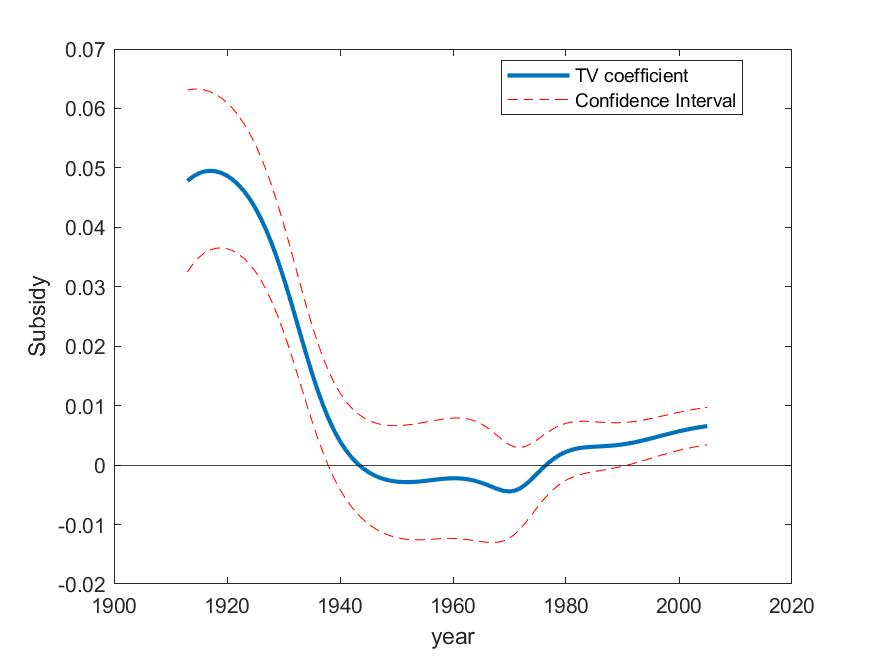
\includegraphics[width=\linewidth]{CI_n201.jpg}
		\end{subfigure}
		\label{chapter 1_1}
	\end{figure}
	
	To justify that our time-varying model specifies a nonlinear cointegrating relationship between tax benefits and general fertility rate, we apply the KPSS stationarity test statistic to the residual of the regression. As the residual is stationary at 10\% level, the instability present in the cointegrating relation shown in Figure \ref{chapter 1_1} is large enough to change the conclusion of no linear cointegration. 
	%\begin{table}[!htp]
	%	\centering
	%	\caption{KPSS Test Results }
	%	\begin{tabular}{ll}
	%		\toprule
	%		& \multicolumn{1}{c}{Subsidy} \\
	%		\midrule
	%		Test Statistics & \multicolumn{1}{c}{0.0971} \\
	%		%        \midrule
	%		%        10\% Critical Value & \multicolumn{1}{c}{0.347} & \multicolumn{1}{c}{0.0885} & \multicolumn{1}{c}{0.0971} \\
	%		Conclusion & \multicolumn{1}{c}{Stationary} \\
	%		\midrule
	%		\multicolumn{2}{l}{\textit{\footnotesize{Note: The 10\% critical value is 0.347. }}} \\
	%	\end{tabular}%
	%	\label{tab:addlabel}%
	%\end{table}%
	
	
	
	\subsection*{Chapter 2}
	
	Previous studies in the empirical literature have taken nonlinearities into account when modeling financial and macroeconomic series (see for example \cite{lettau2008reconciling}, \cite{qi1999nonlinear}). As financial and macroeconomics time-series data are usually non-stationary, subsequent studies have developed estimation methods for the nonlinear univariate econometric models with non-stationary regressors (\cite{park1999asymptotics,park2000nonstationary,park2001nonlinear}).
	%
	However, when extending the univariate framework to include multivariate predictors, it suffers from the curse of dimensionality
	problem because the limiting distribution would naturally be a function of a d-dimensional vector Brownian motion process. As the dimension of multiple predictor increases, the vector Brownian motion process is known to exhibit increasing spatial
	behaviour (\cite{revuz2013continuous}). To avoid this problem, we present an econometric model in which the multiple integrated regressors can be reduced to a univariate single-index form via a known univariate nonlinear function.
	
	We then propose a nonstationary nonlinear single-index model. This model: (a) accounts for the nonlinearities in the data when forecasting next period's macroeconomic and financial variables; (b) helps ease the curse of dimensionality when it comes to parametric nonlinear function estimation involving multivariate integrated regressors; and (c) allows for the presence of cointegrated regressors or non-cointegrated regressors.
	
	%This model can handle a wide variety of nonlinear relationships between the regressand and the single-index component containing either
	%the cointegrated predictors or the non-cointegrated predictors. 
	
	We introduce a new estimation procedure for the model and investigate its finite-sample properties via Monte Carlo simulations. This model is then used to examine stock return predictability via various combinations of integrated lagged economic and financial variables.
	
	\subsubsection*{Model and Methodology}
	This chapter considers the estimation of a nonstationary nonlinear single-index predictive regression model of the form:
	\begin{equation}
		y_{t}=f\left( x_{t-1}^{\prime }\theta _{0},\gamma _{0}\right) +e_{t},\ \ \
		t=2,...,T, 
		\label{chapter_2_model}
	\end{equation}
	where $f\left( .,.\right) $ is a known univariate function, $x_{t-1}$ is a $d
	$-dimensional integrated process of order one, $\theta _{0}$ is a $d$%
	-dimensional unknown true parameter vector that lies in the parameter set $%
	\Theta $, $\gamma _{0}$ is a $m$-dimensional unknown true parameter vector
	that lies in the parameter set $\Gamma $ and $e_{t}$ is a martingale
	difference process. The parameter sets $\Theta $ and $\Gamma $ are assumed
	to be compact and convex subsets of $\mathbb{R}^{d}$ and $\mathbb{R}^{m}$
	respectively.
	
	The linear combination $x_{t-1}^{\prime }\theta _{0}$ in (\ref{chapter_2_model}) is
	called the single-index component. Since $x_{t-1}$ is a vector of $I(1)$ time series, we impose the following two assumptions on the single-index component. The first assumption rules out cointegration among the predictors, $x_{t-1}$, and $\theta_{0}$ the vector of
	single-index coefficients. By contrast, the second assumption permits cointegrated predictors via $x_{t-1}^{\prime }\theta _{0}\sim
	I\left( 0\right) $ with $\theta _{0}$ being the cointegrating vector. 
	
	To illustrate the role played by the parameter vector $\gamma _{0}=\left( \gamma
	_{1,0},...,\gamma _{m,0}\right) ^{\prime }$ in (\ref{model}), consider the
	case where $y_{t}$ is related to the single-index component through a
	quadratic functional form%
	\[
	f\left( u_{t-1},\gamma _{0}\right) =\gamma _{1,0}+\gamma
	_{2,0}u_{t-1}+\gamma _{3,0}u_{t-1}^{2},
	\]%
	where $u_{t-1}=x_{t-1}^{\prime }\theta _{0}.$ Here $\gamma _{0}$ is the
	vector of coefficients for the single-index components. Non-zero elements of 
	$\gamma _{0}$ indicate that the single-index component is a useful predictor of $y_{t}$.
	
	Model (\ref{chapter_2_model}) can be estimated by minimizing sum-of-squared-errors:
	
	\begin{equation*}
		\left( \widehat{\theta},\widehat{\gamma}\right) =\arg \min_{\theta \in \Theta
			,\gamma \in \Gamma }Q_{T}\left( \theta ,\gamma \right) .  
	\end{equation*}%
	where $\left( \widehat{\theta},\widehat{\gamma}\right)$ is the nonlinear least square (NLS) estimator. 
	
	In an attempt to improve the finite sample properties of the NLS estimator, we truncate the squared-errors $\left( y_{t}-f\left(
	x_{t-1}^{\prime }\theta ,\gamma \right) \right) ^{2}$ and we impose a constraint on the coefficient vector $\theta $ in the estimation procedure. To this end, we define the modified sum-of-squared-errors by%
	\begin{equation}
		Q_{T,M}\left( \theta ,\gamma \right) =\sum_{t=1}^{T}\left( y_{t}-f\left(
		x_{t-1}^{\prime }\theta ,\gamma \right) \right) ^{2}I\left( \left\Vert
		x_{t-1}\right\Vert \leq M_{T}\right) +\lambda \left( \left\Vert \theta
		\right\Vert ^{2}-1\right) ,  
		\label{c2_CLS}
	\end{equation}%
	where $I\left( .\right) $ denotes the indicator function, $%
	\left\Vert .\right\Vert $ is the Euclidean norm and $M_T$ = $\sqrt{T}$. It is a positive and increasing sequence satisfying $ M_{T}\rightarrow \infty $ as $T \rightarrow \infty $ and $\lambda $ is a Lagrange
	multiplier. We then obtain the constrained least squares (denoted CLS) estimator $\tilde{\theta }$ and $\tilde{\gamma}$ by minimizing (\ref{c2_CLS}).
	
	We investigate the finite sample properties of the NLS and the proposed CLS estimators in multivariate nonstationary settings. The simulation results show that both NLS and CLS estimators have a good finite sample performance. In addition, there is significant finite sample gains from imposing the constraint on the estimation procedure when comparing the NLS estimator with the CLS estimator.
	
	\subsubsection*{Empirical Study}
	When predicting stock returns, \cite{welch2008comprehensive} find that the linear predictive models predict poorly out-of-sample than a simple model with constant means. We aim to examine whether the single-index predictive model, which explicitly allows for nonlinearities, can produce better out-of-sample fits than the historical average benchmark.We find that several combinations of the predictors used in prior studies deliver out-of-sample forecasting gains relative to the standard historical average benchmark when using the single-index predictive model that accounts for the nonlinearities in the time-series data.
	
	
	\subsection*{Chapter 3}
	In this chapter, we are interested in a partially nonlinear single-index models of the form:
	$$
	y_{t} = \beta_0^{\prime} z_t + g\left( x_{t-1}^{\prime }\theta_0; \gamma_0\right) +e_{t},\ \ \
	t=2,...,T, 
	$$
	where $z_t = (y_{t-1}, \cdots, y_{t-p}, w_{t-1}^{\prime})^{\prime}$, in which $w_{t-1}$ is a vector of stationary predictors, 
	$g\left( .,.\right) $ is a known univariate nonlinear function, $x_{t-1}$ is a $d$-dimensional integrated process of order one, $\theta _{0}$, $\gamma _{0}$ are unknown d-dimensional and m-dimensional true parameter vectors, and $e_{t}$ is a martingale difference process.
	
	Our model allows for lagged dependent variables because key macroeconomic/financial variables, such as the growth rate of GDP, the rate of unemployment and interest rates, are typically autocorrelated. Our model may also be useful in cases where there are additional stationary predictors, $w_{t-1}$, for which the linear specification fits the data better than the nonlinear specification.
	
	To reduce computational burden, we propose a novel 2-step estimation method in which $\beta$ will have a closed form solution while $\theta$ and $\gamma$ can be estimated by the method of nonlinear least squares or constrained nonlinear least squares. In the coming year, I am going to investigate the finite sample properties of the proposed estimator via a Monte Carlo experiment. In the empirical analysis, we will apply the partially nonlinear single-index predictive model to predict stock returns. 
	%both of which are non-stationary time series. In my second year, I continue to work on how to deal with non-stationary time series in an empirical analysis. 
	
	%There are two chapters in this report. The first chapter discusses a non-stationary parametric single-index predictive model. This model can handle a wide variety of nonlinear relationships between the regressand and the single-index component containing either the cointegrated predictors or the non-cointegrated predictors. This model is then used to examine stock return predictability via various combinations of integrated lagged economic and financial variables. The second chapter extends this model by considering a partially nonlinear single-index model. This latter model allows for the inclusion of lagged dependent variables, and allows for a linear relationship between the stationary predictors and the regressand. For both models, we introduce new estimation procedures and investigate their finite-sample properties. 
	
	
	%For both models, we develop new estimation procedures and find good finite sample properties via Monte Carlo experiments. The empirical analysis also suggests that forecasts generated from the first model perform better than the usual historical average benchmark in some consecutive periods. 
	\pagebreak
	
	\tableofcontents{}
	\pagebreak
	%
	%For my future research, I will continue the study on the partial linear single-index model and conduct an empirical analysis of stock return predictability. 
	
	
	%\begin{titlepage}
	%    \begin{center}
	%
	%        {\Large Non-stationary Parametric Single-Index Predictive Models}
	%
	%        \vspace{0.2in}
	
	%        {{\sc Ying Zhou}, {\sc Hsein Kew}, and {\sc Jiti Gao}}
	%
	%     	\vspace{0.1in}
	%	
	%		    \textit{Department of Econometrics and Business Statistics}
	%	
	%		    \textit{Monash University}
	%	
	%	    \vspace{0.1in}
	%
	%        \today
	
	%        \vspace{0.3in}
	
	%        \textbf{Abstract}
	%
	%    \end{center}
	%
	%This paper considers the estimation of a parametric single-index predictive regression model with integrated predictors. This model can handle a wide variety of nonlinear relationships between the regressand and the single-index component containing either the cointegrated predictors or the non-cointegrated predictors. We introduce a new estimation procedure for the model and investigate its finite-sample properties via Monte Carlo simulations. This model is then used to examine stock return predictability via various combinations of integrated lagged economic and financial variables. 
	%
	%
	%\vspace{2in}
	%
	%
	%\textit{Keywords}: Nonlinearity; Nonstationarity; Single-Index Model; Stock Return Predictability.
	
	%\textit{JEL classification}: C13, C14, C32, C51
	
	%\end{titlepage}
	\setcounter{chapter}{1}
	\chapter{Non-stationary Parametric Single-Index Predictive Models}
	
	
	\section{Introduction}
	There is a considerable practical and theoretical effort being channelled into predicting stock returns. Early studies (\cite{campbell1988dividend}, \cite{fama1990stock}, \cite{pesaran1995predictability}) claim that stock returns can be predicted by lagged macroeconomic and financial variables using linear models, while the out-of-sample (OOS) forecasts fail to outperform the historical average (\cite{welch2008comprehensive}). Many different models have since been proposed to find a better OOS forecast; for example, \cite{lee2015forecasting} and \cite{chen2016predictability}) have proposed nonparametric predictive models. Also \cite{dangl2012predictive} and \cite{johannes2014sequential} have developed time-varying coefficients predictive models. 
	
	%In our study, we adopt a single-index predictive model to incorporate the nonlinear relationship between stock return and its predictors. 
	%We use Monte Carlo simulation technique to show the good finite sample properties of the estimators and apply a recursive window scheme in the empirical section to compare the OOS forecast with historical average. 
	
	%\textbf{Literature review}
	
	Previous studies in the empirical literature have taken nonlinearities into account when forecasting financial and macroeconomic series (\cite{lettau2008reconciling}, \cite{qi1999nonlinear}). To account for this nonlinearity feature, a wide variety of nonlinear econometric models has been developed under the assumption that the regressors are stationary. However, financial and macroeconomics time-series data are usually non-stationary and cointegrated. Subsequent studies have developed estimation methods for the nonlinear econometric models with non-stationary regressors. For instance,  \cite{wooldridge1994estimation} and \cite{andrews1995nonlinear} develop an asymptotic theory of estimation for stationary time series around a deterministic (but not stochastic) trend function. In a series of papers, \cite{park1999asymptotics},  \cite{park2000nonstationary}, \cite{park2001nonlinear} develop an asymptotic theory for a class of nonlinear regressions with integrated scalar regressors. These papers continue the work of \cite{park1988statistical} and  \cite{park1989statistical} on linear models in which the regressor is an integrated time series. \cite{chang2001nonlinear} and \cite{chang2003index} extend the non-linear models to allow for multiple integrated regressors. Also, \cite{park2002nonstationary} and \cite{chung2007nonstationary} develop an asymptotic theory for nonlinear heteroskedastic models.
	
	%\textbf{Motivation}
	
	Building on this growing literature, our study focuses on a parametric single-index predictive model with integrated regressors. This model: (a) accounts for the nonlinearities in the data when forecasting next period's macroeconomic and financial variables; (b) helps ease the curse of dimensionality when it comes to parametric nonlinear function estimation involving multivariate integrated regressors; and (c) allows for the presence of cointegrated regressors or non-cointegrated regressors. Our work is related to the semi-parametric single-index framework used by \cite{dong2016estimation} in which the integrated predictors are not cointegrated, and by \cite{zhou2018semiparametric} in which the integrated predictors are cointegrated (see also \cite{xu2016testing}, \cite{lee2018lasso} and \cite{koo2020high}). 
	
	In our parametric specification, we develop a new estimation procedure for the single-index model and show, via a Monte Carlo experiment, that it has better finite sample properties than the usual nonlinear least-squares estimator. In our empirical analysis, we use the single-index model containing multivariate integrated regressors to predict future stock returns. Our results suggest that forecasts generated from this model perform better than the usual historical average benchmark in an out-of-sample forecasting exercise when we account for the nonlinear relationship between stock returns and the multivariate integrated predictors. 
	
	This chapter is organised as follows. Section 2 introduces the parametric single-index predictive model and presents a parametric estimator for this model. Section 3 examines the small-sample properties of the estimators by a Monte Carlo  evaluation. The application to stock market return predictability is given in Section 4. Section 5 concludes. 
	
	\section{Parametric Single-Index Predictive Model}
	
	In this chapter, we study the estimation for a parametric single-index predictive model with nonstationary predictors%
	\begin{equation}
		y_{t}=f\left( x_{t-1}^{\prime }\theta _{0},\gamma _{0}\right) +e_{t},\ \ \
		t=2,...,T,  \label{model}
	\end{equation}%
	where $f\left( .,.\right) $ is a known univariate function, $x_{t-1}$ is a $d
	$-dimensional integrated process of order one, $\theta _{0}$ is a $d$%
	-dimensional unknown true parameter vector that lies in the parameter set $%
	\Theta $, $\gamma _{0}$ is a $m$-dimensional unknown true parameter vector
	that lies in the parameter set $\Gamma $ and $e_{t}$ is a martingale
	difference process. The parameter sets $\Theta $ and $\Gamma $ are assumed
	to be compact and convex subsets of $\mathbb{R}^{d}$ and $\mathbb{R}^{m}$
	respectively. In order to ensure that $\theta_0$ is uniquely identifiable, we will need to impose $\theta_{0}^{\prime}\theta_{0} = 1$.
	
	The linear combination $x_{t-1}^{\prime }\theta _{0}$ in (\ref{model}) is
	called the single-index component. Since $x_{t-1}$ is a vector of $I(1)$ time series, we impose the following two assumptions on the single-index component. The first assumption rules out cointegration among the predictors, $x_{t-1}$, and $\theta_{0}$ the vector of
	single-index coefficients. By contrast, the second assumption permits cointegrated predictors via $x_{t-1}^{\prime }\theta _{0}\sim
	I\left( 0\right) $ with $\theta _{0}$ being the cointegrating vector. 
	
	Our single-index predictive model can be used to predict stock market returns without imposing linearity. The most commonly used predictors, such as dividend-price ratio, earning-price ratio, book-to-market ratio, term spread and dividend-payout ratio, have been found to be non-stationary and often contain an autoregressive unit root; see Table 7 of \cite{kostakis2015robust} and Table 4 of \cite{campbell2006efficient}. \cite{campbell2004caught} estimate a linear trivariate predictive model containing earning-price ratio, term spread and book-to-market ratio as predictors. In the absence of a cointegrating relationship among these predictors, we could utilize this single-index model to re-examine the out-of-sample forecasting performance of these predictors. In the cointegrated predictors case, \cite{lettau2001consumption} consider $x_{t-1}=\left( c_{t-1},a_{t-1},y_{t-1}\right)^{\prime }$ where $c_{t}$ is log
	consumption, $a_{t}$ is log asset wealth and $y_{t}$ is log labor income. They show that, under the general household budget constraint framework, the predictors $c_{t}$, $a_{t}$ and $y_{t}$ should move together over the long run and are hence cointegrated. They suggest that the cointegrating residual (termed the `cay' variable) from regressing $c_{t-1}$ on $a_{t-1}$ and $y_{t-1}$ is a relevant predictor of stock returns when using a linear predictive model. Again, we could utilize this single-index model to re-assess the forecasting ability of the cointegrated cay predictor. 
	
	%They estimate the cointegrating relationship between these predictors and
	
	To illustrate the role played by the parameter vector $\gamma _{0}=\left( \gamma
	_{1,0},...,\gamma _{m,0}\right) ^{\prime }$ in (\ref{model}), consider the
	case where $y_{t}$ is related to the single-index component through a
	quadratic functional form%
	\[
	f\left( u_{t-1},\gamma _{0}\right) =\gamma _{1,0}+\gamma
	_{2,0}u_{t-1}+\gamma _{3,0}u_{t-1}^{2},
	\]%
	where $u_{t-1}=x_{t-1}^{\prime }\theta _{0}.$ Here $\gamma _{0}$ is the
	vector of coefficients for the single-index components. Non-zero elements of 
	$\gamma _{0}$ indicate that the single-index component is a useful predictor of $y_{t}$. The single-index model (\ref{model}) includes as a special case the simple neural network model -- with $f\left( u_{t-1},\gamma _{0}\right) =\gamma _{1,0}+\gamma _{2,0}G\left(
	\gamma _{3,0}+u_{t-1}\right) $ for a known function $G\left( .\right) $ -- considered by \cite{chang2003index}. 
	
	
	%\textcolor{red}{Kew to add papers that deal with stationary x for estimation.}
	%\textcolor{red}{Kew to add Park Phillips 2000 ecta on nonstationary binary choice model here.}
	
	In the case where $x_{t-1}$ is a univariate integrated
	predictor, \cite{park2001nonlinear} consider a parametric nonlinear nonstationary
	regression model: $y_{t}=f\left( x_{t-1},\gamma _{0}\right) +e_{t}.$
	They use a nonlinear least squares (NLS) estimator to estimate their model
	and show that the limiting distribution of this estimator is a functional of a univariate Brownian motion. An extension of their univariate framework to include multivariate predictors suffers from the curse of dimensionality problem because the limiting distribution would naturally be a function of a $d$-dimensional vector Brownian motion. As the dimension of $x_{t}$ increases, the vector Brownian motion process is known to exhibit increasing
	spatial behaviour; see \cite{revuz2013continuous}. The use of the single-index method avoids this spatial problem because it reduces the dimension of multivariate predictors to a univariate linear combination $x_{t-1}^{\prime
	}\theta _{0},$ and thereby eliminates the necessity for vector Brownian motion in the development of the limit theory.
	
	
	Following \cite{chang2003index}, the single-index model (\ref{model}) can be estimated by a NLS estimator. Define the sum-of-squared-errors by%
	\[
	Q_{T}\left( \theta ,\gamma \right) =\sum_{t=1}^{T}\left( y_{t}-f\left(
	x_{t-1}^{\prime }\theta ,\gamma \right) \right) ^{2}. 
	\]%
	The NLS estimator $\hat{\theta}$ and $\hat{\gamma}$ is given by minimizing $%
	Q_{T}\left( \theta ,\gamma \right) $ over $\theta \in \Theta $ and $\gamma
	\in \Gamma ,$ that is%
	\begin{equation}
		\left( \widehat{\theta},\widehat{\gamma}\right) =\arg \min_{\theta \in \Theta
			,\gamma \in \Gamma }Q_{T}\left( \theta ,\gamma \right) .  \label{nls}
	\end{equation}%
	
	The solutions to (\ref{nls}) must be found numerically because there is no
	closed-form solution. The `\textit{nloptr}' package in R with Augmented Lagrangian Algorithm can be used as an optimization routine to numerically solve (\ref{nls}).
	
	
	%\textcolor{teal}{The "\textit{fminunc}" routine of the Matlab software package with Gauss-Newton algorithm can be used as an optimization routine to numerically solve (\ref{nls}). Do we need to change this because we used R? Maybe we can write: The "nloptr" package in R with Augmented Lagrangian Algorithm can be used as an optimization routine to numerically solve (\ref{nls})}
	
	
	
	In an attempt to improve the finite sample properties of the NLS estimator, we truncate the squared-errors $\left( y_{t}-f\left(
	x_{t-1}^{\prime }\theta ,\gamma \right) \right) ^{2}$ and we impose a constraint on the coefficient vector $\theta $ in the estimation procedure. To this end, we define the modified sum-of-squared-errors by%
	\begin{equation}
		Q_{T,M}\left( \theta ,\gamma \right) =\sum_{t=1}^{T}\left( y_{t}-f\left(
		x_{t-1}^{\prime }\theta ,\gamma \right) \right) ^{2}I\left( \left\Vert
		x_{t-1}\right\Vert \leq M_{T}\right) +\lambda \left( \left\Vert \theta
		\right\Vert ^{2}-1\right) ,  
		\label{mSSE}
	\end{equation}%
	where $I\left( .\right) $ denotes the indicator function, $%
	\left\Vert .\right\Vert $ is the Euclidean norm and $M_T$ = $\sqrt{T}$. It is a positive and increasing sequence satisfying $ M_{T}\rightarrow \infty $ as $T \rightarrow \infty $ and $\lambda $ is a Lagrange
	multiplier. 
	
	The reason for truncating the squared-errors $\left( y_{t}-f\left(
	x_{t-1}^{\prime }\theta ,\gamma \right) \right) ^{2}$ in (\ref{mSSE}) is that the presence
	of integrated predictors will tend to produce far too few observations at distinct spatial locations. These observations may cause a standard
	optimisation routine to fail to converge when solving (\ref{nls}). 
	This truncation method was originally used by \cite{li2016estimation} for the case when the univariate regressor $x_{t-1}$ follows the null recurrent Markov process, which is known to exhibit spatial structure. 
	
	
	The constrained least squares (denoted CLS) estimator $\widetilde{\theta}$ and $%
	\widetilde{\gamma}$ is given by minimizing $Q_{T,M}\left( \theta ,\gamma \right) 
	$ over $\theta \in \Theta $ and $\gamma \in \Gamma $ such that the
	restriction $\left\Vert \theta \right\Vert ^{2}=1$ holds; that is%
	\begin{equation}
		\left( \widetilde{\theta},\widetilde{\gamma}\right) =\arg \min_{\theta \in \Theta
			,\gamma \in \Gamma ,\left\Vert \theta \right\Vert ^{2}=1}Q_{T,M}\left(
		\theta ,\gamma \right) .  \label{cls}
	\end{equation}%
	A constrained optimization method is required to find the solutions to (\ref{cls}) and the `\textit{nloptr}' package in R can still be used to numerically solve (\ref{cls}) subject to the constraint that $\left\Vert \theta \right\Vert ^{2}=1.$
	
	%The `nloptr' package in R
	
	%A constrained optimization method is required to find the solutions to (\ref%{cls}) and the `\textit{fmincon}' routine of the Matlab software package canbe used to numerically solve (\ref{cls}) subject to the constraint that $%\left\Vert \theta \right\Vert ^{2}=1.$
	
	The constraint $\left\Vert \theta \right\Vert ^{2}=1
	$ in (\ref{mSSE}) scales the CLS estimator to the surface of
	the unit ball and \cite{zhou2018semiparametric} demonstrate that, in their semi-parametric single-index model, this constraint on the estimation procedure causes the CLS estimator of $\theta _{0}$ to converge to their true values at a faster rate than that for the case without contraints. In our parametric single-index model, the simulation results in the next section show significant finite sample gains from imposing this constraint on the estimation procedure when comparing the NLS estimator 
	with the CLS estimator. 
	
	\section{Monte Carlo Simulation }
	\subsection{Data Generation Process}
	In this section, we investigate the finite sample properties of the NLS and the proposed CLS estimators in multivariate nonstationary settings. The predictors $x_{t-1}$ is a $2$-vector integrated time series. Data were generated on the following models:%
	\begin{eqnarray}
		\label{DGP}
		y_{t} &=&f\left( x_{t-1}^{\prime }\theta _{0},\gamma _{0}\right) +e_{t},\ \
		e_{t}\sim i.i.d. N\left( 0,1\right) , \nonumber \\
		x_{t} &=& x_{t-1}+v_{t}, \ \ x_{0}=\left( 0,0\right) ^{\prime }, \nonumber \\
		v_{t} &=&\left(\begin{array}{c}
			v_{1, t} \\
			v_{2, t}
		\end{array}\right) \sim i.i.N\left(\left(\begin{array}{c}
			0 \\
			0
		\end{array}\right),\left(\begin{array}{cc}
			1 & 0.5 \nonumber \\
			0.5 & 1
		\end{array}\right)\right).
	\end{eqnarray}
	We consider the following nonlinear functions:%
	\begin{eqnarray}
		\label{functions}
		f_{1}\left( u,\gamma _{0}\right) &=&\sin \left( u+\gamma _{1,0}\right), \nonumber \\
		f_{2}\left( u,\gamma _{0}\right) &=&\cos \left( u+\gamma _{1,0}\right), \nonumber \\
		f_{3}\left( u,\gamma _{0}\right) &=& 1-e^{-\gamma_{1,0}\left(u-\gamma_{2,0}\right)^{2}}, \\
		f_{4}\left( u,\gamma _{0}\right) &=& \gamma_{1,0} e^{-\gamma_{2,0}u^2},\nonumber  \\
		f_{5}\left( u,\gamma _{0}\right) &=&\gamma_{1,0}+\gamma_{2,0}u+\gamma _{3,0}u^{2}. \nonumber 
	\end{eqnarray}%
	with $\gamma_{1,0}= 0.2,\gamma_{2,0}= 0.3$ and $\gamma_{3,0}= 0.3.$ The first four functions are bounded on $\mathbb{R}$ and the last one is
	unbounded on $\mathbb{R}$. 
	
	We consider sample sizes $T=100,500,1000$ and we use $M = 1000$ simulation  replications. In the CLS estimation method, we follow \cite{li2016estimation} by choosing $M_{T}=\sqrt{T}$. Let $\theta_0=\left( \theta%
	_{1,0},\theta_{2,0}\right) ^{\prime }$. To evaluate the finite sample performance of the NLS and proposed CLS estimators, we compute the bias and standard deviation of each element of $\hat{\theta}$ and $\tilde{\theta}$ defined in the previous section. For example, let $\widehat{\theta}=\left( \widehat{\theta}_{1},\widehat{\theta}_{2}\right) ^{\prime }$ and $\widehat{\theta}_{i}^{(j)}$ denote the $j$-th replication of
	the estimate $\widehat{\theta}_{i}$ for $i = 1,2$. Then, for the NLS estimator, we have%
	\[
	\text{bias}=\overline{\widehat{\theta}}_{i}-\theta _{i,0}, 
	\]%
	where $\overline{\widehat{\theta}}_{i}=M^{-1}\sum_{j=1}^{M}\widehat{\theta}_{i}^{(j)} $; and  
	\[
	\text{standard deviation (s.d.)}=\sqrt{M^{-1}\sum_{j=1}^{M}\left( \widehat{\theta}_{i}^{(j)}-\overline{\widehat{\theta}}_{i}\right) ^{2}}. 
	\]%
	Since $\widehat{\theta}_1$ and $\widehat{\theta}_{2}$ are correlated, we also calculate a type of estimated covariance of the form:
	\begin{equation}
		\label{std of theta}
		\sigma_{\theta}=\frac{1}{M} \sum_{j=1}^{M}\left(\widehat{\theta}_{1}^{(j)}-\overline{\widehat{\theta}}_{1}\right)\left(\widehat{\theta}_{2}^{(j)}-\overline{\widehat{\theta}}_{2}\right), \quad \text { std}_{\theta}=|\sigma_{\theta}|.
	\end{equation}
	%\textcolor{red}{Kew to ask Jiti where does this $\sigma_{\theta}$ comes from? do we have a paper to cite about this? No worries, if not. But it would be good to give a bit of interpretation for this $\sigma_{\theta}$ }
	
	\subsection{Computational Details}
	In this section, we provide an instruction on how to estimate the parameters using CLS estimation. In equation (\ref{mSSE}), $\left( \left\Vert \theta\right\Vert ^{2}-1\right)$ is an equality constraint that only applies to the parameter $\theta$ and we use nonlinear least square method with Lagrange multiplier to estimate both $\theta$ and $\gamma$. To simplify, we first denote the Lagrangian multiplier as:
	
	$$
	L_{n,m}\left( \theta ,\gamma,\lambda\right) =\sum_{t=1}^{T}F_t(\theta ,\gamma) +\lambda h(\theta)
	$$
	where $F_t(\theta ,\gamma) = \left( y_{t}-f\left(x_{t-1}^{\prime }\theta ,\gamma \right) \right) ^{2}I\left( \left\Vert
	x_{t-1}\right\Vert \leq M_{T}\right)$ and $h(\theta)=\left( \left\Vert \theta \right\Vert ^{2}-1\right)$.
	
	The necessary conditions for an extremum of $F_t$ with the equality constraints $h(\theta)=0$ are that:
	\begin{equation}
		\nabla L((\theta^{*},\gamma^{*}), \lambda^{*})=\left[\begin{array}{c}
			\nabla_{\lambda} L(\lambda^{*}, \theta, \gamma) \\
			\nabla_{\theta} L(\theta^{*}, \gamma, \lambda) \\
			\nabla_{\gamma} L(\gamma^{*}, \theta, \lambda) 
		\end{array}\right]
		= 
		\left[\begin{array}{c}
			\frac{\partial L}{\partial \lambda}\\
			\frac{\partial L}{\partial \theta}\\
			\frac{\partial L}{\partial \gamma}
		\end{array}\right]
		= 0
		\label{gradient}
	\end{equation} 
	where $\frac{\partial L}{\partial \lambda} = \frac{\partial h}{\partial \lambda}$, $\frac{\partial L}{\partial \theta} = \left(\frac{\partial F_t}{\partial \theta_1} \frac{\partial F_t}{\partial \theta_2} \cdots \frac{\partial F_t}{\partial \theta_d}\right)^{T}$, and $\frac{\partial L}{\partial \gamma} = \left(\frac{\partial F_t}{\partial \gamma_1} \frac{\partial F_t}{\partial \gamma_2} \cdots \frac{\partial F_t}{\partial \gamma_m}\right)^{T}$.
	
	Given that condition (\ref{gradient}) is satisfied, we then move on to check whether the Hessian matrix with a Lagrangian multiplier (or bordered Hessian) is negative definite. Bordered hessian is given below:
	
	\begin{equation}
		\mathbf{H}(L)=\left[\begin{array}{ccc}
			\frac{\partial^{2} L}{\partial \lambda^{2}} & \frac{\partial^{2} L}{\partial \lambda \partial \theta} & \frac{\partial^{2} L}{\partial \lambda \partial \gamma} \\
			\left(\frac{\partial^{2} L}{\partial \lambda \partial \theta}\right)^{\top} & \frac{\partial^{2} L}{\partial \theta^{2}} & \frac{\partial^{2} L}{\partial \theta \partial \gamma} \\ \left(\frac{\partial^{2} L}{\partial \lambda \partial \gamma}\right)^{\top} & \left(\frac{\partial^{2} L}{\partial \theta \partial \gamma}\right)^{\top} & \frac{\partial^{2} L}{\partial \gamma^{2}}
		\end{array}\right] = \left[\begin{array}{ccc}
			0 & \frac{\partial^{2} L}{\partial \lambda \partial \theta} & \frac{\partial^{2} L}{\partial \lambda \partial \gamma} \\
			\left(\frac{\partial^{2} L}{\partial \lambda \partial \theta}\right)^{\top} & \frac{\partial^{2} L}{\partial \theta^{2}} & \frac{\partial^{2} L}{\partial \theta \partial \gamma} \\ \left(\frac{\partial^{2} L}{\partial \lambda \partial \gamma}\right)^{\top} & \left(\frac{\partial^{2} L}{\partial \theta \partial \gamma}\right)^{\top} & \frac{\partial^{2} L}{\partial \gamma^{2}}
		\end{array}\right]
	\end{equation}
	
	So if $(-1) det(H(L)) >0$, then L has a local minimum. As an example, consider the functional form:
	
	$$
	f_{1}\left( u,\gamma\right) =\sin \left( u+\gamma\right), u = (\theta_1 x_1 + \theta_2 x_2).
	$$
	The first order optimality condition is given by:
	
	\begin{equation*}
		\nabla L((\theta^{*},\gamma^{*}), \lambda^{*})=\left[\begin{array}{c}
			\nabla_{\lambda} L(\lambda^{*}, \theta, \gamma) \\
			\nabla_{\theta} L(\theta^{*}, \gamma, \lambda) \\
			\nabla_{\gamma} L(\gamma^{*}, \theta, \lambda) 
		\end{array}\right]
		= 
		\left[\begin{array}{c}
			\theta_1^{2} + \theta_2^{2} -1 \\
			-\sum_{t=1}^{T} (y - f_{1}\left( u,\gamma\right))\frac{\partial f_{1}\left( u,\gamma\right)}{\partial \theta_1} + 2\lambda \theta_1\\
			-\sum_{t=1}^{T} (y - f_{1}\left( u,\gamma\right))\frac{\partial f_{1}\left( u,\gamma\right)}{\partial \theta_2} + 2\lambda \theta_2\\
			-\sum_{t=1}^{T} (y - f_{1}\left( u,\gamma\right))\frac{\partial f_{1}\left( u,\gamma\right)}{\partial \gamma}
		\end{array}\right]
		= 0
		\label{gradient cal}
	\end{equation*} 
	where I denote the truncation condition: $I\left( \left\Vert x_{t-1}\right\Vert \leq M_{T}\right)$.
	
	The second order condition, that is the Hessian matrix is given by:
	
	\begin{equation*}
		\mathbf{H}(L)=
		%\left[\begin{array}{ccc}
		%\frac{\partial^{2} L}{\partial \lambda^{2}} & \frac{\partial^{2} L}{\partial \lambda \partial \theta} & \frac{\partial^{2} L}{\partial \lambda \partial \gamma} \\
		%\left(\frac{\partial^{2} L}{\partial \lambda \partial \theta}\right)^{\top} & \frac{\partial^{2} L}{\partial \theta^{2}} & \frac{\partial^{2} L}{\partial \theta \partial \gamma} \\ \left(\frac{\partial^{2} L}{\partial \lambda \partial \gamma}\right)^{\top} & \left(\frac{\partial^{2} L}{\partial \theta \partial \gamma}\right)^{\top} & \frac{\partial^{2} L}{\partial \gamma^{2}}
		%\end{array}\right] = 
		\left[\begin{array}{cccc}
			0 & -2\theta_1 & -2\theta_2 & 0 \\
			-2\theta_1 & D_{\theta_1\theta_1} + 2\lambda & D_{\theta_1\theta_2} & D_{\theta_1\gamma}\\ -2\theta_2 & D_{\theta_2\theta_1} & D_{\theta_2\theta_2} + 2\lambda & D_{\theta_2\gamma}\\
			0 & D_{\gamma\theta_1}  & D_{\gamma\theta_2} & D_{\gamma\gamma}
		\end{array}\right]
	\end{equation*}
	where 
	$D_{\alpha\beta} = \sum_{t=1}^{T} \frac{\partial f_{1}\left( u,\gamma\right)}{\partial \alpha} \left( \frac {\partial f_{1}\left( u,\gamma\right)}{\partial \beta}\right) ^{\prime} - \sum_{t=1}^{T}\left( y_t - f_{1}\left( u,\gamma\right)\right)  \frac{\partial^{2} f_{1}\left( u,\gamma\right)}{\partial \alpha^2}.$
	
	%$D_{\theta_1\theta_1} = \sum_{t=1}^{T} \frac{\partial f_{1}\left( u,\gamma\right)}{\partial \delta} \left( \frac {\partial f_{1}\left( u,\gamma\right)}{\partial \delta}\right) ^{\prime} - \sum_{t=1}^{T}\left( y_t - f_{1}\left( u,\gamma\right)\right)  \frac{\partial^{2} f_{1}\left( u,\gamma\right)}{\partial \delta^2} + 2\lambda$
	%
	%$D_{\theta_1\theta_2} = D_{\theta_2\theta_1} =  \frac{\partial^{2} L}{\partial \theta_1 \partial \theta_2} = 2cos(u+\gamma)\cdot x_1 x_2 \cdot I \cdot (cos(u+\gamma) + 2(y - sin(u+\gamma)))$
	%
	%$D_{\theta_2\theta_2} = \sum_{t=1}^{T} \frac{\partial f(v_t; \delta)}{\partial \delta} \left( \frac {\partial f(v_t; \delta)}{\partial \delta}\right) ^{\prime} - \sum_{t=1}^{T}\left( y_t - f(v_t;\delta)\right) \frac{\partial^{2} f(v_t; \delta)}{\partial \delta^2} + 2\lambda$
	%
	%$D_{\theta_1\gamma} = \frac{\partial^{2} L}{\partial \theta_1 \partial \gamma} = 2 x_1 \cdot I \cdot (cos^2(u+\gamma) + 2 (y - sin(u+\gamma))sin(u+\gamma))$
	%
	%$D_{\theta_2\gamma} = \frac{\partial^{2} L}{\partial \theta_2 \partial \gamma} = 2 x_2 \cdot I \cdot (cos^2(u+\gamma) + 2 (y - sin(u+\gamma))sin(u+\gamma))$
	%
	%$D_{\gamma\theta_1} = \frac{\partial^{2} L}{\partial \gamma \theta_1} = 2x_1\cdot I \cdot (cos^2(u+\gamma) + y\cdot sin(u+\gamma) -sin^2(u+\gamma))$
	%
	%$D_{\gamma\theta_1} = \frac{\partial^{2} L}{\partial \gamma \theta_2} = 2x_1\cdot I \cdot (cos^2(u+\gamma) + y\cdot sin(u+\gamma) -sin^2(u+\gamma))$
	%
	%$D_{\gamma\gamma} = \frac{\partial^{2} L}{\partial \gamma^2} = 2y \cdot I \cdot cos(u+\gamma)$
	
	Then we can check the sign of det(H(L)) to decide whether a local minimum exists. If there is a local minimum, we can find it by solving (\ref{gradient cal}).
	
	
	\subsection{Simulation Results}
	We first consider the case in which the predictors are not cointegrated, so that the single-index component $x_{t-1}^{\prime }\theta _{0}$ is purely non-stationary by setting $\theta_{0} =\left( 0.8,0.6\right) ^{\prime }$. The simulation results are reported in Table \ref{Table CLS}. As we can see, the biases, standard deviations and $\sigma_{\theta}$ for the NLS and CLS estimators decrease as the sample size increases. These results are promising, and indicate that both NLS and CLS are consistent estimators of $\theta _{0}.$ Table \ref{Table CLS} also shows that our proposed CLS estimator exhibits a much better finite sample performance than the NLS estimator, especially much smaller finite sample biases and standard deviations across all experiments. Take the function $f_1(u, \gamma_{0})$ in Table (\ref{Table CLS}) as an example, when T = 100, the bias of $\theta_{1,0}$ decreases from 0.01497 to 0.00422 when comparing the NLS and CLS estimators. It is thus useful to incorporate the truncation method and impose a constraint on the coefficient vector $\theta $ in the estimation procedure. 
	
	We now allow for the possibility of cointegration among the predictors by setting $\theta_{0} =\left( 0.6,-0.8\right) ^{\prime }$ and hence the single-index component $x_{t-1}^{\prime }\theta _{0}$ becomes $I(0)$. We also allow the predictors $x_{t-1}$ to follow a vector integrated process driven by an MA(1) innovations; that is  
	$$v_t = \epsilon_t + C\epsilon_{t-1},$$
	where $\epsilon_{t} \sim i.i.d. N\left(\left(\begin{array}{c}
		0 \\
		0
	\end{array}\right)
	,\left(\begin{array}{cc}1 & 0.5 \\ 0.5 & 1\end{array}\right)\right)$ and $C=\left(\begin{array}{cc} -1  & 4/ 3 \\ 0 & 0\end{array}\right)$. 
	
	%where $\epsilon_{t} \sim i i N\left(0,\left(\begin{array}{cc}1 & 0.5 \\ 0.5 & %1\end{array}\right)\right)$ and $C=\left(\begin{array}{cc} -1  & 4/ 3 \\ 0 & %0\end{array}\right)$. 
	
	We report simulation results in Table \ref{Table 3} only for the CLS estimator since in the non-cointegrated case we find that there are finite sample gains when resorting to a constrained estimation procedure. As can be seen, the performance of the CLS estimator tends to improve as the sample size increases across the different regression functions. Deriving the theoretical properties of the CLS estimator under both non-cointegrated and cointegrated predictors should be a good topic for future research. 
	
	
	%Similarly, the standard deviation of $\theta$ also decreases when we consider Simulation results for cointegrated case is reported in Table \ref{cointegrated}. We only report results for the CLS estimator since in the non-cointegrated case we already find that there are finite sample gains when resorting to a constrained estimation procedure. In Table \ref{Table 3}, all the estimators show very good finite sample properties. Both bias and standard deviation drop when sample size becomes larger. For example, for the polynomial function $f_5(u, \gamma_{0})$, the bias drops to 0.00004 when T = 1000. 
	
	
	\begin{table}[htbp]
		\centering
		\caption{Finite sample properties of NLS and CLS estimators: Non-cointegrated predictors}
		\label{Table CLS}
		\begin{adjustbox}{max width=0.95\textwidth}
			\begin{tabular}{clcccccccc}
				\hline \hline
				&   &   & \multicolumn{3}{c}{CLS} & \multicolumn{3}{c}{NLS} \\
				&   &   & \textbf{T=100} & \textbf{T=500} & \textbf{T=1000} & \textbf{T=100} & \textbf{T=500} & \textbf{T=1000} \\
				\hline
				
				\multirow{6}[0]{*}{$f_1(u,\gamma_{0})$} &\multirow{2}[0]{*}{$\theta_{1,0}$} & Bias  & 0.00422 & 0.00112 & 0.00038 & 0.01497 & 0.00532 & 0.00369 \\
				&	& s.d.  & 0.02191 & 0.00600 & 0.00365 & 0.08951 & 0.04345 & 0.03039 \\
				&\multirow{2}[0]{*}{$\theta_{2,0}$} & Bias  & -0.00068 & -0.00013 & -4.5E-05 & -0.00227 & -0.00250 & 0.00200 \\
				&	& s.d.  & 0.00271 & 0.00061 & 0.00037 & 0.15105 & 0.06067 & 0.04121 \\
				&	& $std_{\theta}$  & 0.00845 & 0.00689 & 0.00137 & 0.10982 & 0.07392 & 0.03368 \\
				&\multirow{2}[0]{*}{$\gamma_{1,0}$} & Bias  & -0.00779 & -0.00032 & -0.00152 & 0.00582 & 0.00326 & 0.00266 \\
				&	& s.d.  & 0.17540 & 0.07832 & 0.05733 & 0.13945 & 0.05851 & 0.04129 \\
				
				\hline
				
				\multirow{6}[0]{*}{$f_2(u,\gamma_{0})$} & \multirow{2}[0]{*}{$\theta_{1,0}$} & Bias & 0.00447 & 0.00139 & 0.00064 & -0.00128 & -0.00016 & -0.00011 \\
				&   & s.d. & 0.023040 & 0.00642 & 0.00336 & 0.03094 & 0.00755 & 0.00390 \\
				& \multirow{2}[0]{*}{$\theta_{2,0}$} & Bias & -0.00073 & -0.00016 & -7E-05 & -0.00058 & -0.00003 & -0.00010 \\
				&   & s.d. & 0.00292 & 0.00066 & 0.00034 & 0.02912 & 0.00722 & 0.00386 \\
				&	& $std_{\theta}$  & 0.00845 & 0.00689 & 0.00137 & 0.11256 & 0.29867 & 0.01399 \\
				& \multirow{2}[0]{*}{$\gamma_{1,0}$} & Bias & -0.00211 & -0.0057 & -0.00161 & 0.04223 & 0.00609 & -0.00229 \\
				&   & s.d. & 0.16254 & 0.08333 & 0.05583 & 0.09154 & 0.04721 & 0.02063 \\
				
				
				\hline
				
				\multirow{8}[0]{*}{$f_3(u,\gamma_{0})$} & \multirow{2}[0]{*}{$\theta_{1,0}$} & Bias & -0.00011 & -0.00005 & 0.00007 & 0.00634 & 0.00409 & 0.00380 \\
				&   & s.d. & 0.00371 & 0.00312 & 0.00254 & 0.02708 & 0.01484 & 0.01076 \\
				& \multirow{2}[0]{*}{$\theta_{2,0}$} & Bias & 0.00007 & 0.00003 & -0.00006 & 0.06275 & 0.01113 & 0.00459 \\
				&   & s.d. & 0.00267 & 0.00225 & 0.00195 & 0.19590 & 0.07324 & 0.05620 \\
				&	& $std_{\theta}$  & 0.00345 & 0.00279 & 0.00011 & 0.03922 & 0.00981 & 0.00136\\
				& \multirow{2}[0]{*}{$\gamma_{1,0}$} & Bias & -0.00083 & 0.00460 & 0.00861 & 0.01342 & 0.00349 & 0.00185 \\
				&   & s.d. & 0.02793 & 0.14505 & 0.16913 & 0.03588 & 0.0.00877 & 0.00576 \\
				& \multirow{2}[0]{*}{$\gamma_{2,0}$} & Bias & 0.09702 & 0.07387 & 0.03148 & 0.03655 & 0.01197 & 0.00696 \\
				&   & s.d. & 1.21163 & 0.90087 & 0.51446 & 0.05355 & 0.02329 & 0.01733 \\
				
				
				\hline \hline
			\end{tabular}%
		\end{adjustbox}
	\end{table}%
	
	
	\begin{table}[htbp]
		\centering
		\caption*{Table \ref{Table CLS}: Continued}
		\begin{adjustbox}{max width=0.95\textwidth}
			\begin{tabular}{clcccccccc}
				\hline \hline
				&   &   & \multicolumn{3}{c}{CLS} & \multicolumn{3}{c}{NLS} \\
				& \multicolumn{1}{l}{} &   & \textbf{T=100} & \textbf{T=500} & \textbf{T=1000} & \textbf{T=100} & \textbf{T=500} & \textbf{T=1000} \\
				\hline
				
				
				\multirow{8}[1]{*}{$f_4(u,\gamma_{0})$} & \multirow{2}[1]{*}{$\theta_{1,0}$} & Bias & -0.00047 & -0.00054 & -0.00028 & 0.03116 & 0.03489 & 0.02974 \\
				&   & s.d. & 0.03926 & 0.00974 & 0.00485 & 0.41504 & 0.15343 & 0.10855 \\
				& \multirow{2}[0]{*}{$\theta_{2,0}$} & Bias & -0.00049 & 0.00012 & 4E-05 & -0.00729 & 0.01939 & 0.01315 \\
				&   & s.d. & 0.02934 & 0.00853 & 0.00444 & 0.37102 & 0.14480 & 0.08879 \\
				&	& $std_{\theta}$  & 0.00552 & 0.00398 & 0.00275 & 0.00992 & 0.00584 & 0.00412 \\
				& \multirow{2}[0]{*}{$\gamma_{1,0}$} & Bias & 0.00288 & -0.00023 & -0.00011 & 0.01621 & -0.00864 & -0.00925 \\
				&   & s.d. & 0.02392 & 0.00738 & 0.00336 & 0.09407 & 0.05596 & 0.03377 \\
				& \multirow{2}[0]{*}{$\gamma_{2,0}$} & Bias & 0.00171 & -0.00087 & -0.00009 & -0.00210 & 0.00759 & 0.01689 \\
				&   & s.d. & 0.03928 & 0.00664 & 0.00874 & 0.37198 & 0.16559 & 0.11484 \\
				
				\hline
				
				\multirow{10}[0]{*}{$f_5(u,\gamma_{0})$} & \multirow{2}[0]{*}{$\theta_{1,0}$} & Bias & -0.00077 & -0.00001 & 0.00000 & 0.00237 & 0.00167 & 0.00094 \\
				&   & s.d. & 0.00571 & 0.00090 & 0.00041 & 0.01033 & 0.00494 & 0.00326 \\
				& \multirow{2}[0]{*}{$\theta_{2,0}$} & Bias & 0.00006 & 0.00000 & 0.00000 & 0.00220 & 0.00139 & 0.00068 \\
				&   & s.d. & 0.00053 & 0.00009 & 0.00004 & 0.01132 & 0.00483 & 0.00329\\			
				&	& $std_{\theta}$  & 0.00053 & 0.00019 & 0.00008 & 0.00444 & 0.00192 & 0.00107 \\
				& \multirow{2}[0]{*}{$\gamma_{1,0}$} & Bias & -0.00071 & 0.00167 & 0.00168 & -0.00003 & -0.00049 & -0.00013 \\
				&   & s.d. & 0.01609 & 0.00513 & 0.00322 & 0.00809 & 0.00296 & 0.00214 \\
				& \multirow{2}[0]{*}{$\gamma_{2,0}$} & Bias & 0.00008 & 0.00000 & 0.00000 & -0.00174 & -0.00111 & -0.00062 \\
				&   & s.d. & 0.00472 & 0.00060 & 0.00028 & 0.00446 & 0.00238 & 0.00148 \\
				& \multirow{2}[0]{*}{$\gamma_{3,0}$} & Bias & 0.00014 & -0.00003 & -0.00001 & 0.00270 & 0.00107 & 0.00045 \\
				&   & s.d. & 0.00595 & 0.00084 & 0.00040 & 0.00581 & 0.00358 & 0.00233 \\
				
				\hline \hline
			\end{tabular}%
		\end{adjustbox}
	\end{table}%
	
	
	
	% Table generated by Excel2LaTeX from sheet 'cos'
	\begin{table}[htbp]
		\centering
		\caption{Finite sample properties of CLS estimator: Cointegrated predictors}
		\label{Table 3}
		\begin{adjustbox}{max width=1.1\textwidth}
			\begin{tabular}{cc|rrccrrrrcc}
				\toprule
				&       & \multicolumn{3}{c|}{$f_1(u,\gamma_{0})$} & \multicolumn{3}{c|}{$f_2(u,\gamma_{0})$} & \multicolumn{4}{c}{$f_3(u,\gamma_{0})$}   \\
				&       & \multicolumn{1}{c}{$\gamma_{1,0}$} & \multicolumn{1}{c}{$\theta_{1,0}$} & \multicolumn{1}{c|}{$\theta_{2,0}$} & $\gamma_{1,0}$ & \multicolumn{1}{c}{$\theta_{1,0}$} & \multicolumn{1}{c|}{$\theta_{2,0}$} & \multicolumn{1}{c}{$\gamma_{1,0}$} & \multicolumn{1}{c}{$\gamma_{2,0}$} & $\theta_{1,0}$ & $\theta_{2,0}$ \\
				\midrule
				\multirow{3}[1]{*}{T = 100} & bias  & -0.00707 & 0.00814 & \multicolumn{1}{r|}{-0.03127} & \multicolumn{1}{r}{-0.00511} & 0.00815 & \multicolumn{1}{r|}{-0.02885} & -0.01325 & 0.03478 & \multicolumn{1}{r}{0.02894} & \multicolumn{1}{r}{0.56838} \\
				& std   & 0.05976 & 0.08368 & \multicolumn{1}{r|}{0.22101} & \multicolumn{1}{r}{0.05561} & 0.07984 & \multicolumn{1}{r|}{0.19458} & 0.18462 & 0.25850 & \multicolumn{1}{r}0.39893{} & \multicolumn{1}{r}{0.86347} \\
				& $std_{\theta}$ &       & \multicolumn{2}{c|}{0.21981} &       & \multicolumn{2}{c|}{0.19987} &       &       & \multicolumn{2}{c}{0.05635} \\
				\multirow{3}[0]{*}{T = 500} & bias  & -0.00049 & 0.00065 & \multicolumn{1}{r|}{-0.00102} & \multicolumn{1}{r}{-0.00115} & 0.00124 & \multicolumn{1}{r|}{-0.00589} & -0.01193 & -0.03216 & \multicolumn{1}{r}{0.02289} & \multicolumn{1}{r}{0.11934} \\
				& std   & 0.01789 & 0.02420 & \multicolumn{1}{r|}{0.07311} & \multicolumn{1}{r}{0.01135} & 0.01536 & \multicolumn{1}{r|}{0.05785} & 0.06733 & 0.08842 & \multicolumn{1}{r}{0.0.07056} & \multicolumn{1}{r}{0.21906} \\
				& $std_{\theta}$ &       & \multicolumn{2}{c|}{0.07272} &       & \multicolumn{2}{c|}{0.06180} &       &       & \multicolumn{2}{c}{0.01955} \\
				
				\multirow{3}[1]{*}{T = 1000} & bias  & -0.00007 & 0.00083 & \multicolumn{1}{r|}{-0.00120} & \multicolumn{1}{r}{-0.00066} & 0.00075 & \multicolumn{1}{r|}{-0.00257} & -0.00434 & 0.00793 & \multicolumn{1}{r}{0.00173} & \multicolumn{1}{r}{0.09899} \\
				& std   & 0.00812 & 0.01115 & \multicolumn{1}{r|}{0.04286} & \multicolumn{1}{r}{0.00764} & 0.01072 & \multicolumn{1}{r|}{0.03726} & 0.01899 & 0.03194 & \multicolumn{1}{r}{0.03956} & \multicolumn{1}{r}{0.09878} \\
				& $std_{\theta}$ &       & \multicolumn{2}{c|}{0.04471} &       & \multicolumn{2}{c|}{0.03731} &       &       & \multicolumn{2}{c}{0.01266} \\
				\midrule
				&       & \multicolumn{4}{c}{$f_4(u,\gamma_{0})$}        &       & \multicolumn{5}{c}{$f_5(u,\gamma_{0})$} \\
				&       & \multicolumn{1}{c}{$\gamma_{1,0}$} & \multicolumn{1}{c}{$\gamma_{2,0}$} & $\theta_{1,0}$ & $\theta_{2,0}$ &       & \multicolumn{1}{c}{$\gamma_{1,0}$} & \multicolumn{1}{c}{$\gamma_{2,0}$} & \multicolumn{1}{c}{$\gamma_{3,0}$} & $\theta_{1,0}$ & $\theta_{2,0}$ \\
				\midrule
				\multirow{3}[1]{*}{T = 100} & bias  & 0.04778 & -0.05835 & \multicolumn{1}{r}{0.42574} & \multicolumn{1}{r}{0.44352} &       & 0.00244 & -0.00290 & 0.00176 & \multicolumn{1}{r}{-0.00725} & \multicolumn{1}{r}{-0.02559} \\
				& std   & 0.22502 & 30026 & \multicolumn{1}{r}{79131} & \multicolumn{1}{r}{1.35994} &       & 0.00982 & 0.01532 & 0.02586 & \multicolumn{1}{r}{0.09341} & \multicolumn{1}{r}{0.05667} \\
				& $std_{\theta}$ &       &       & \multicolumn{2}{c}{0.09709} &       &       &       &       & \multicolumn{2}{c}{0.10301} \\
				
				\multirow{3}[0]{*}{T = 500} & bias  & -0.00359 & 0.00408 & \multicolumn{1}{r}{0.09030} & \multicolumn{1}{r}{17635} &       & 0.00041 & -0.00047 & 0.00077 & \multicolumn{1}{r}{-0.00025} & \multicolumn{1}{r}{-0.00352} \\
				& std   & 0.07905 & 0.10786 & \multicolumn{1}{r}{0.32777} & \multicolumn{1}{r}{0.69730} &       & 0.00386 & 0.00609 & 0.00896 & \multicolumn{1}{r}{0.03894} & \multicolumn{1}{r}{0.02578} \\
				& $std_{\theta}$ &       &       & \multicolumn{2}{c}{0.04742} &       &       &       &       & \multicolumn{2}{c}{0.05841} \\
				
				\multirow{3}[1]{*}{T = 1000} & bias  & -0.00266 & 0.00241 & \multicolumn{1}{r}{0.05001} & \multicolumn{1}{r}{0.07098} &       & 4.37E-05 & -0.00027 & 0.00008 & \multicolumn{1}{r}{-0.00049} & \multicolumn{1}{r}{-0.00103} \\
				& std   & 0.05233 & 0.07447 & \multicolumn{1}{r}{0.23882} & \multicolumn{1}{r}{0.37198} &       & 0.00266 & 0.00418 & 0.00532 & \multicolumn{1}{r}{0.02730} & \multicolumn{1}{r}{0.03349} \\
				& $std_{\theta}$ &       &       & \multicolumn{2}{c}{0.008577438} &       &       &       &       & \multicolumn{2}{c}{0.03156} \\
				\bottomrule
				\bottomrule
			\end{tabular}%
		\end{adjustbox}
		\label{cointegrated}%
	\end{table}%
	
	\section{Empirical illustration: Stock market return predictability}
	
	%regression model that contains only a constant term when we account for the nonlinear relationship between stock returns and the predictors. by capturing some of the nonlinearities in the data.  
	
	
	To illustrate the use of the single-index model, we provide an application to predictability of U.S. stock market returns. We focus on out-of-sample forecasts because it involves forecasters making predictions in real time (\cite{stock2007has}). There is a large and growing empirical literature that attempts to predict stock returns using lagged macroeconomic and financial
	variables. Most empirical studies in this literature have focused on univariate linear predictive regression models, including, for example, the papers by  \cite{campbell1987stock}, \cite{fama1989business}, \cite{pesaran1995predictability} and \cite{choi2016reexamination}. However, several subsequent papers argue that multiple predictors can explain the variation in stock returns better than a single predictor because multivariate predictive models are less prone to suffer from omitted predictors problem (\cite{cochrane2011presidential}). 
	
	%For example, \cite{ang2007stock} uses the combination of dividend-price ratio and T-bill rate to predict the stock returns. \cite{campbell2004caught} specify a multivariate predictive regression model with earning-price ratio, book-to-market ratio and term spread. \cite{lamont1998earnings} uses a bivariate predictive regression model with dividend-price ratio and payout ratio.
	
	%In all these papers, a linear specification is used for 
	
	%The commonly used predictors are typically non-stationary and cointegrated. For example \cite{kostakis2015robust}, Campbell and Yogo. Weilun, Bonsoo, Zhentao and Keli Xu provide evidence of cointegrated predictors. Mr Weilun find evidence of nonlinear relations between stock returns and the single-index component. Also \cite{qi1999nonlinear} and \cite{abhyankar1997uncovering} show that nonlinear predictive models perform better than the sample mean model. \textcolor{red}{Maybe delete this paragraph or re-write or put somewhere else.}
	
	A linear specification for the bivariate/multivariate predictive regression is used in many empirical applications. However, \cite{welch2008comprehensive} find that the linear predictive models predict poorly out-of-sample than a simple model with constant means. Meanwhile \cite{qi1999nonlinear} and \cite{zhou2018semiparametric} find evidence of nonlinearities in the stock return and lagged financial variables relationship. The main objective of this section is to examine whether the parametric single-index model, which explicitly allows for nonlinearities in the predictive relations, can produce better out-of-sample fits than the historical average benchmark. 
	
	The dataset used for this study is available from Amit Goyal's website. The examined period is quarterly data from 1956:Q1 to 2018:Q4. The dependent variable, $y_t$, is the equity premium defined as the S\&P500 value-weighted log excess returns. We select a combination of predictors $x_{t-1}$ that has been found to be important, both theoretically and empirically, in prior studies of stock return predictability. Table 7 of \cite{kostakis2015robust} provides evidence suggesting that the commonly used predictors contain a unit root. Using the Engle-Granger test for cointegration, we fail to reject the null hypothesis of no cointegration for the following combinations of predictors: (a) dividend-price ratio and T-bill rate, see \cite{ang2007stock}; (b) dividend-price ratio, T-bill rate, default yield spread and term spread, see \cite{ferson1996measuring}; (c) dividend-price ratio and book-to-market ratio, see \cite{kothari1997book}; (d) dividend-price ratio and dividend-payout ratio,  see \cite{lamont1998earnings}, and (e) earning-price ratio, term spread and book-to-market ratio, see \cite{campbell2004caught}. The following four combinations of cointegrated predictors are considered in \cite{zhou2018semiparametric}: (f) dividend-price ratio and dividend yield; (g) T-bill rate and long-term yield; (h) dividend-price ratio and earning-price ratio; (i) baa- and aaa-rated corporate bond yields; and (j) $c_t$, $a_t$ and $y_t$, see \cite{lettau2001consumption}. 
	
	We use the same regression functions (namely $f_{1}\left( u,\gamma\right), f_{2}\left( u,\gamma\right), f_{3}\left( u,\gamma\right), f_{4}\left( u,\gamma \right)$ and $f_{5}\left( u,\gamma\right)$) as in the Monte Carlo section. The single-index model is estimated using the CLS estimator with $M_{T}=\sqrt{T}$.  We consider one-step ahead forecasting of the equity premium using all the 10 combinations of predictors and the 5 nonlinear functions, for a total of 50 single-index predictive models. We generate pseudo out-of-sample forecasts from a sequence of recursive predictions. 
	
	We evaluate the out-of-sample performance using a recursive window scheme. The details are described as follows. We divide the total observations $T$ into in-sample part containing $T_1$ observations from Q1 of 1956 to Q4 of 1987, while the remaining $T-T_1$ observations from Q1 of 1988 to Q4 of 2018 are regarded as out-of-sample period. To generate the first out-of-sample stock return forecast, we use the first $T_1$-1 pairs of observations \{($x_1$, $y_2$), ($x_2$, $y_3$), $\cdots$, ($x_{T_1-1}$, $y_{T_1}$)\} to estimate the nonlinear model and predict $\hat{y}_{T_1+1}$. We then include the information in the $T_1$+1 period and predict  $\hat{y}_{T_1+2}$ using \{($x_1$, $y_2$), ($x_2$, $y_3$), $\cdots$, ($x_{T_1}$, $y_{T_1+1}$)\}. The procedure continues until we obtain $\hat{y}_{T}$ and the predicted values are denoted by:
	\begin{center}
		$\hat{y}_{T_1+1}$, $\hat{y}_{T_1+2}$, $\cdots$, $\hat{y}_{T}$
	\end{center}
	
	In order to compare the forecast accuracy, we calculate the out-of-sample $R^2$ following the work of \cite{campbell2008predicting} and compute the out-of-sample $R^2$ statistic:
	\[
	R_{OOS}^{2}=1-\frac{T_{2}^{-1}\sum_{s=1}^{T_{2}}\left( y_{T_{1}+s}-\hat{y}%
		_{T_{1}+s}\right) ^{2}}{T_{2}^{-1}\sum_{s=1}^{T_{2}}\left( y_{T_{1}+s}-\bar{y%
		}_{T_{1}+s}\right) ^{2}},
	\]
	where $T_{2} = T- T_{1} $ with $T_{1}$ is the number of observations in the (in-sample) estimation period, $\hat{y}_{t+1} = f\left( x_{t}^{\prime }\tilde{\theta },\tilde{\gamma}\right)$ is the forecast in period $t+1$,  and $\bar{y}_{t+1}=t^{-1}\sum_{s=1}^{t}y_{s}$ is the historical average benchmark forecast. The single-index model has a forecasting performance that beats the benchmark if $ R^2_{OOS}>0 $. We report out-of-sample results in a set of figures that show the $R_{OOS}^{2}$ statistic on the vertical axis and the beginning of the various out-of-sample evaluation periods on the horizontal axis. This will provide us with an assessment of the robustness of the out-of-sample forecasting results.
	
	% in Figures \ref{CV vs SM}, \ref{L vs SM}, \ref{cwyf4} and \ref{cointegrated}. 
	
	Figures 1-4 shows some of the OOS results we have. The red horizontal line represents 0. If the blue line ($ R^2_{OOS}$) lies above the red line, it means the OOS forecasts generated by our nonlinear models outperform the historical average benchmark. Here, we present only the combinations of predictors and nonlinear functions that are found to produce positive $ R^2_{OOS}$ values over a substantial number of out-of-sample periods. 
	
	Figure \ref{CV vs SM} and Figure \ref{L vs SM} show that for some non-cointegrated predictors studied previously,  when using $f_3\left( u,\gamma\right)$ as a nonlinear function, the following combinations of predictors generate out-of-sample gains: (a) earning-price ratio, book-to-market ratio and term spread (see Figure \ref{CV vs SM}); (b) dividend-price ratio and dividend-payout ratio (see Figure \ref{L vs SM}). In particular, Figure \ref{CV vs SM} shows that the multivariate predictors generate consecutive out-of-sample gains after 2014. 
	
	
	%We examine the forecasting performance of the single-index model based on out-of-sample prediction generated from a sequence of recursive procedures. 
	
	%\subsection{OOS Results of Combinations from Previous Studies}
	%The 2 pictures come from table 5 respectively.
	
	%Figure \ref{CV vs SM} shows the OOS forecasting results of combination CV using $f_3$, compared with sample mean model.
	
	%Figure \ref{L vs SM} shows the OOS forecasting results of combination L using $f_3$
	
	
	\begin{figure}[!htb]
		\begin{minipage}{0.48\textwidth}
			\centering
			\captionsetup{justification=centering,margin=0cm}
			\caption{Predictors: earning-price ratio, book-to-market ratio, term spread and $f_{3}( u,\gamma)$ }
			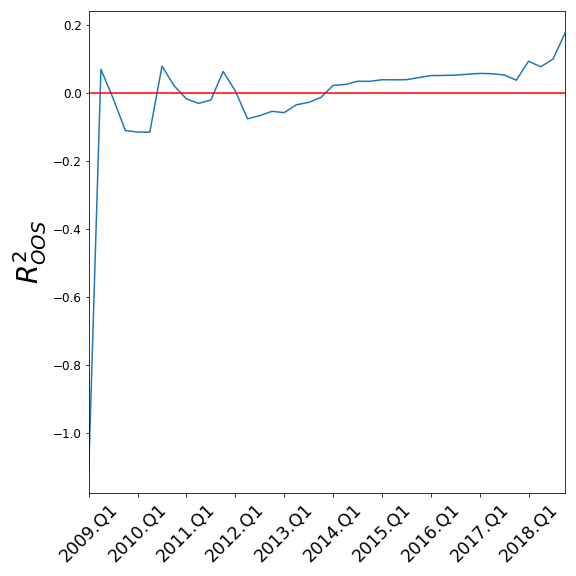
\includegraphics[width=0.9\linewidth]{CV.png}
			
			\label{CV vs SM}%
		\end{minipage}\hfill
		\begin{minipage}{0.48\textwidth}
			\centering
			\captionsetup{justification=centering,margin=0cm}
			\caption{Predictors: dividend price, dividend-payout and $f_{3}( u,\gamma )$ }
			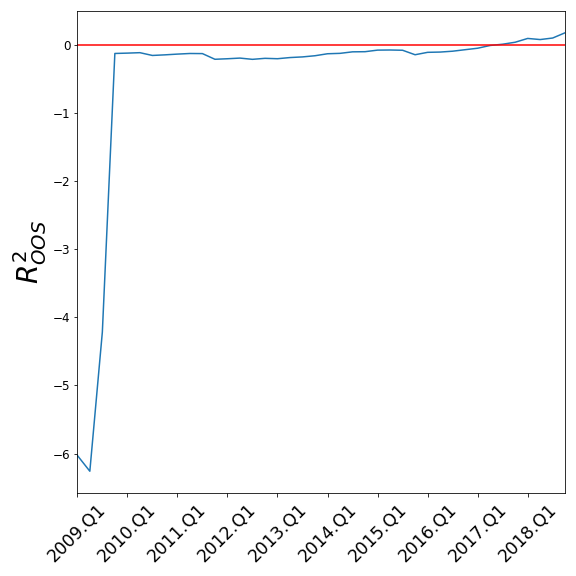
\includegraphics[width=0.9\linewidth]{L.png}
			
			\label{L vs SM}%
		\end{minipage}
	\end{figure}
	
	The result presented in Figure \ref{cwyf4} is obtained using the 3 cointegrated predictors $c_{t-1}$, $a_{t-1}$ and $y_{t-1}$ and using $f_3\left( u,\gamma\right)$. These predictors have been studied in \cite{lettau2001consumption} and we find that, using our model, this combination of cointegrated predicotrs generates better forecasts than the historical average benchmark around the year 2000 and at the end of the forecasting period. 
	
	%The same predictors have been studied in \cite{lettau2001consumption}, in which they first regress  $c_{t-1}$ on $a_{t-1}$ and $y_{t-1}$, and then show that the cointegrating residual has a good predictability. In our study, by using single-index model, we can show the predictability of  $c_{t-1}$, $a_{t-1}$ and $y_{t-1}$ in one step.
	
	\begin{figure}[H]
		\centering
		\captionsetup{justification=centering}
		\caption{Predictors: log consumption, log asset wealth and log labor income and  $f_{3}( u,\gamma)$ }
		\label{cwyf4}%
		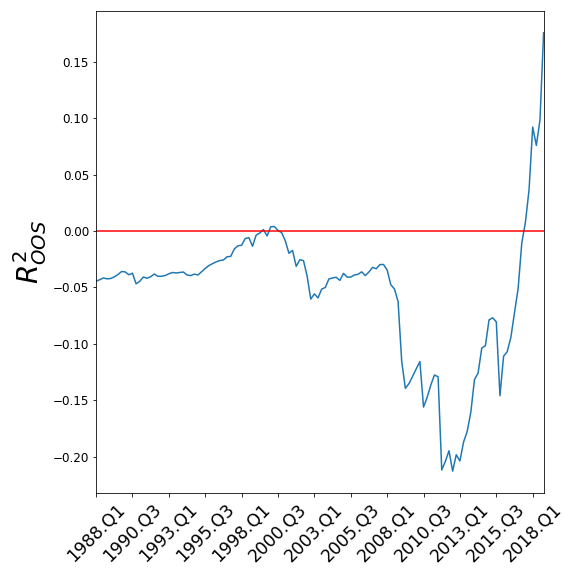
\includegraphics[width=0.5\linewidth]{cwy(f4).png}
	\end{figure}
	
	
	
	\begin{figure}[H] % "[t!]" placement specifier just for this example
		\caption{Forecasting results using cointegrated predictors} 
		\label{cointegrated}
		\begin{subfigure}{0.48\textwidth}
			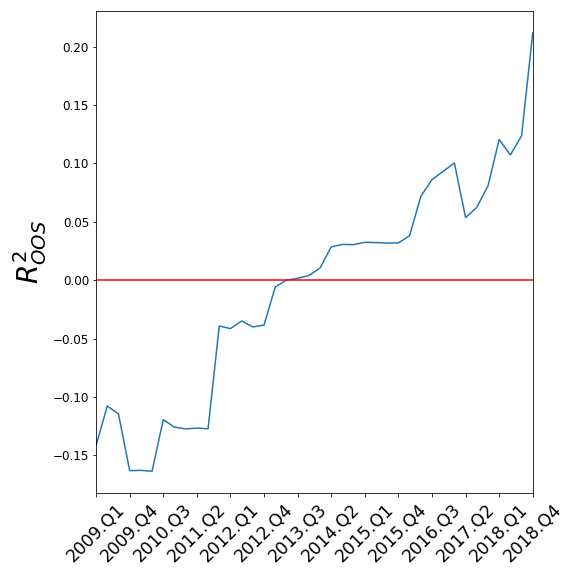
\includegraphics[width=0.8\linewidth]{co2f1.png}
			\captionsetup{justification=centering}
			\caption{Predictors: long-term yield and T-bill rate and $f_{1}( u,\gamma)$ } \label{co2f1}
		\end{subfigure}\hspace*{\fill}
		\begin{subfigure}{0.48\textwidth}
			\captionsetup{justification=centering}
			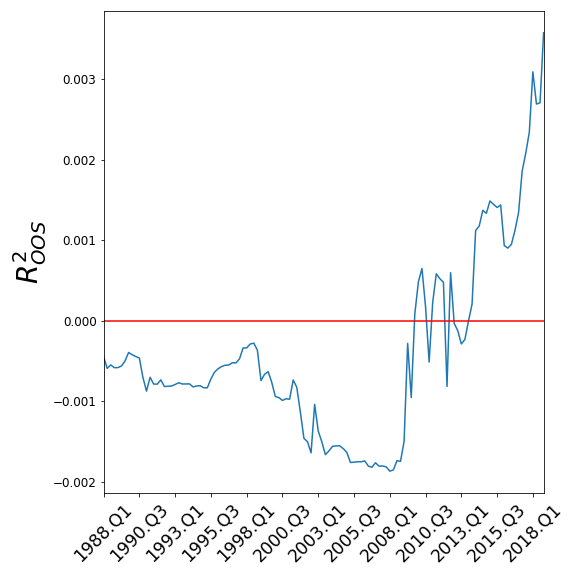
\includegraphics[width=0.8\linewidth]{co2f4.png}
			\caption{Predictors: long-term yield and T-bill rate and $f_{4}( u,\gamma)$ } \label{co2f4}
		\end{subfigure}
		
		\medskip
		\begin{subfigure}{0.48\textwidth}
			\captionsetup{justification=centering}
			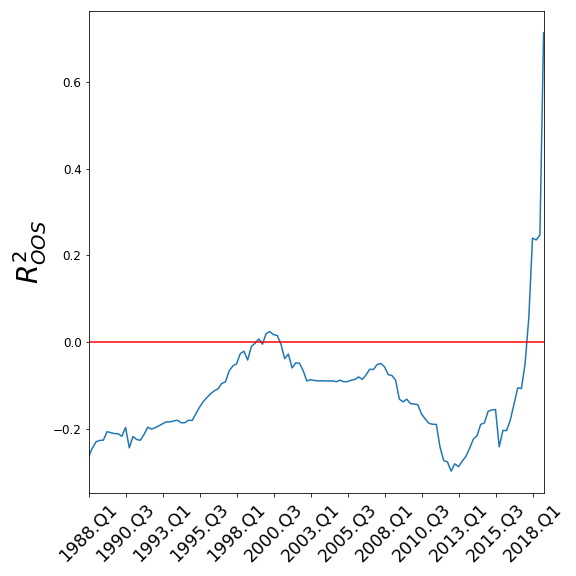
\includegraphics[width=0.8\linewidth]{co2f5.png}
			\caption{Predictors: long-term yield and T-bill rate and $f_{5}( u,\gamma)$ } \label{co2f5}
		\end{subfigure}\hspace*{\fill}
		\begin{subfigure}{0.48\textwidth}
			\captionsetup{justification=centering}
			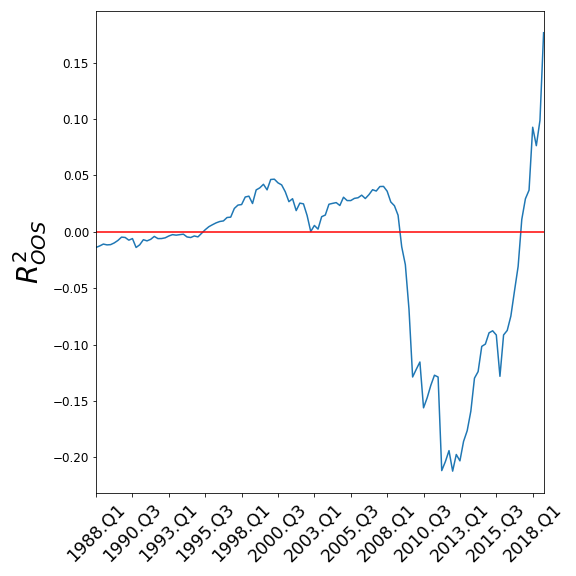
\includegraphics[width=0.8\linewidth]{co1f3.png}
			\caption{Predictors: dividend-price and earning-price and $f_{3}( u,\gamma)$ } \label{co1f3}
		\end{subfigure}
		
		\medskip
		\begin{subfigure}{0.48\textwidth}
			\captionsetup{justification=centering}
			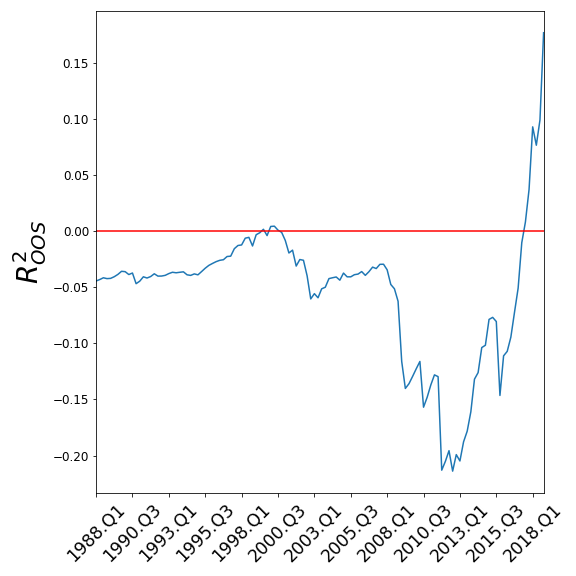
\includegraphics[width=0.8\linewidth]{co3f3.png}
			\caption{Predictors: dividend-price and dividend yield and $f_{3}( u,\gamma)$ } \label{co3f3}
		\end{subfigure}\hspace*{\fill}
		\begin{subfigure}{0.48\textwidth}
			\captionsetup{justification=centering}
			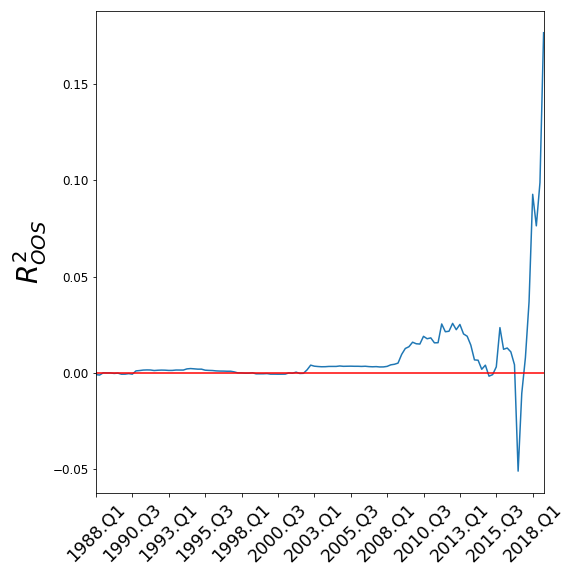
\includegraphics[width=0.8\linewidth]{co4f3.png}
			\caption{Predictors: BAA and AAA and $f_{3}( u,\gamma)$ } \label{co4f3}
		\end{subfigure}
	\end{figure}
	
	Figure \ref{cointegrated} displays the results when we use pairs of cointegrated predictors considered in \cite{zhou2018semiparametric}. As shown in Figure \ref{cointegrated} (a), (b) and (c), the pair of long-term yield and 3-month T-bill rate produces $ R^2_{OOS}>0 $ when using  $f_1\left( u,\gamma\right)$, $f_4\left( u,\gamma\right)$ and $f_5\left( u,\gamma\right)$ as nonlinear functions. The function $f_1\left( u,\gamma\right)$ produces positive $ R^2_{OOS}>0 $ after 2013, while the function  $f_4\left( u,\gamma\right)$ gives consecutive positive results after 2009. We also find that when using $f_3\left( u,\gamma\right)$ as a nonlinear function, the following three pairs of predictors generate positive $R_{OOS}^{2}$ values: (a) dividend-price ratio and earning-price ratio; (b) dividend-price ratio and dividend yield; and (c) baa- and aaa- rated corporate bond yields (see Figures \ref{cointegrated} (c), (d) and (e)). From Figure \ref{cointegrated} (d), we can see that the dividend-price ratio and earning-price ratio not only produce positive $ R^2_{OOS}>0 $ at the end of the forecasting period, but generates consecutive better forecasts from around 1995 to 2008. In Figure \ref{cointegrated} (e), the combination of aaa- and baa- rated corporate bond rates produces long and continuous positive $ R^2_{OOS}>0 $ over the out-of-sample forecasting period.
	
	%Figure \ref{dcwy_f4} and Figure \ref{dcwy4_f2} show us the results from demeaned  $\tilde{c}_{t-1, }\tilde{a}_{t-1}, \tilde{y}_{t-1}$ with cointegrated variable pairs studied in \cite{zhou2018semiparametric}. We demean the $c_{t-1}$, $a_{t-1}$ and $y_{t-1}$ series because it has a dominant deterministic trend. In Figure \ref{dcwy_f4}, we can see that under $f_{4}( u,\gamma)$, the 5-variable combination: the demeaned dividend price ratio, earnings price ratio and demeaned $c_{t-1}$, $a_{t-1}$ and $y_{t-1}$ produces positive $ R^2_{OOS}>0 $ consecutively after 2009. Figure \ref{dcwy4_f2} displays that when baa- and aaa- rated corporate bond yields are combined with the demeaned $c_{t-1}$, $a_{t-1}$ and $y_{t-1}$, they achieve a large OOS gain between 2009 and 2015 using $f_{2}( u,\gamma)$.
	
	These findings indicate that exploiting nonlinearities in the data can lead to improved forecast accuracy relative to the historical average benchmark. Overall, the single-index predictive model shows that the largest out-of-sample forecast gains in all the figures come from using the combination of aaa- and baa- rated corporate bond rates, and using the nonlinear function $f_3\left( u,\gamma\right)$. \\
	
	\section{Conclusion}
	This chapter considers a parametric single-index predictive model with integrated predictors. We propose a new constrained estimation procedure to estimate this model and show that it has better finite sample properties than the usual NLS estimator. We apply the model to examine the predictability of stock returns using cointegrated and non-cointegrated predictors. We find that several combinations of the predictors used in prior studies deliver out-of-sample forecasting gains relative to the standard historical average benchmark over a large number of evaluation periods when using the single-index predictive model that accounts for the nonlinearities in the time-series data. 
	
	\pagebreak
	
	
	\chapter{Partially Nonlinear Single-Index Predictive Models}
	
	\setcounter{section}{0}
	\section{Introduction}
	%Partial-linear model is an important tool for multivariate regression due to its flexibility. It combines linear model with a nonparametric model, which can capture both linear and nonlinear relationship between dependent variable and predictors (see for example \cite{stute2005nonparametric}). Such works include Such works include \cite{chen1988convergence}, \cite{carroll1997generalized} and \cite{ruppert2003semiparametric}. Due to the "curse of dimensionality", the nonlinear relationship in the nonparametric part can be difficult to explore (see for example, \cite{ma2013doubly}). Therefore, we follow \cite{dong2016estimation} and consider a partial linear single-index model of the form:
	
	Conventional partially linear models involving both parametric and nonparametric components have been widely studied in the literature, such as by \cite{gao2007nonlinear}. In the time series literature, partially linear single-index models have also attracted attention in recent years, see for example \cite{dong2016estimation}. We are now interested in a new class of nonlinear time series models - partially nonlinear single-index models of the form:
	\begin{equation}
		y_{t} = \beta_0^{\prime} z_t + g\left( x_{t-1}^{\prime }\theta_0; \gamma_0\right) +e_{t},\ \ \
		t=2,...,T,  \label{PL model}
	\end{equation}%
	where $z_t = (y_{t-1}, \cdots, y_{t-p}, w_{t-1}^{\prime})^{\prime}$, in which $w_{t-1}$ is a vector of stationary predictors, 
	%such as the 3 components (consumption, labour income and asset holdings) of "cay" variable constructed by \textcolor{blue}{Lettau and Ludvigson (2001)}.
	$g\left( .,.\right) $ is a known univariate nonlinear function, $x_{t-1}$ is a $d$-dimensional integrated process of order one, $\theta _{0}$ is a $d$-dimensional unknown true parameter vector that lies in the parameter set $\Theta $, $\gamma _{0}$ is a $m$-dimensional unknown true parameter vector that lies in the parameter set $\Gamma $ and $e_{t}$ is a martingale
	difference process. The parameter sets $\Theta $ and $\Gamma $ are assumed to be compact and convex subsets of $\mathbb{R}^{d}$ and $\mathbb{R}^{m}$ respectively. In order to ensure that $\theta_0$ is uniquely identifiable, we will need to impose $\theta_{0}^{\prime}\theta_{0} = 1$.
	
	Our model allows for lagged dependent variables because key macroeconomic/financial variables, such as the growth rate of GDP, the rate of unemployment and interest rates are typically autocorrelated. Failing to account for this autocorrelation will lead to serially correlated residuals. We are thus interested in using this model to assess whether including lagged dependent variables would, in fact, improve forecasts of $y_{t}$ relative to using only the nonlinear single-index component, $g\left( x_{t-1}^{\prime }\theta_0; \gamma_0\right)$, containing either the cointegrated predictors or non-cointegrated predictors. Our model may also be useful in cases where there are additional stationary predictors, $w_{t-1}$, for which the linear specification fits the data better than the nonlinear specification.
	
	There is a considerable theoretical effort being put into developing new estimation method of the partial linear model (see for example, \cite{dong2016estimation}) and nonlinear models with single-index (see for example \cite{chang2003index}). In our study, we propose a novel 2-step estimation method in which $\beta$ will have a closed form solution while $\theta$ and $\gamma$ can be estimated by the method of nonlinear least squares or constrained nonlinear least squares.
	
	This study aims to use the Monte Carlo simulation method to investigate the finite sample properties of the estimators. There will also be an empirical analysis to study the predictability of stock returns. We will use the dataset from \cite{welch2008comprehensive} and investigate the out-of-sample forecast ability of model (\ref{PL model}). Compared with chapter 2, we will include lagged dependent variables in the model. We will investigate whether the partially nonlinear single-index model will help further improve the stock return predictability in my future research.  
	
	
	
	%One of the motivation of considering this model is the different time series properties in predictors  
	%
	%Model \ref{PL model} considered both stationary and nonstationary time series, especially that the lagged dependent variables have been included in the linear component. In this chapter, we will extend 
	\section{Model and Methodology}
	
	Since in our case, $g\left( x_{t-1}^{\prime }\theta_0; \gamma_0\right)$ is known, model (\ref{PL model}) can be estimated by using a nonlinear least square method. Let $L(\beta, \theta, \gamma) = \sum_{t=1}^{T} \left( y_t - \beta^{\prime} z_t - g\left( x_{t-1}^{\prime }\theta; \gamma\right)\right) ^2$, and hence we have the following score functions:
	
	$$
	\frac{\partial L(\beta, \theta, \gamma)}{\partial \beta} = -2\sum_{t=1}^{T} z_t^{\prime} \left( y_t - \beta^{\prime} z_t - g\left( x_{t-1}^{\prime }\theta; \gamma\right)\right)
	$$
	
	$$
	\frac{\partial L(\beta, \theta, \gamma)}{\partial \theta} = -2\sum_{t=1}^{T} \left( y_t - \beta^{\prime} z_t - g\left( x_{t-1}^{\prime }\theta; \gamma\right)\right)\frac{\partial g(x_{t-1}^{\prime }\theta; \gamma)}{\partial \theta}
	$$
	
	$$
	\frac{\partial L(\beta, \theta, \gamma)}{\partial \gamma} = -2\sum_{t=1}^{T} \left( y_t - \beta^{\prime} z_t - g\left( x_{t-1}^{\prime }\theta; \gamma\right)\right) \frac{\partial g(x_{t-1}^{\prime }\theta; \gamma)}{\partial \gamma}
	$$
	
	The minimum value of $L(\beta, \theta, \gamma)$ occurs when the above score functions equals to 0. Notice that these score functions $\frac{\partial L(\beta, \theta, \gamma)}{\partial \theta}$ and $\frac{\partial L(\beta, \theta, \gamma)}{\partial \gamma}$ are nonlinear functions of both the variables and the parameters, and so they do not have closed form solutions. To estimate the parameters, we need to include an iterative procedure and obtain optimal values by using gradient descent algorithms. However, recognising that this score function $\frac{\partial L(\beta, \theta, \gamma)}{\partial \beta}$ is linear in the parameter $\beta$, we introduce a novel two-step approach for estimation in order to reduce the computational burden. 
	
	In step 1, we set $\frac{\partial L(\beta, \theta, \gamma)}{\partial \beta} = 0$. Solve the equation and we have:
	\begin{equation}
		\hat{\beta} = \left( \sum_{t=1}^{T}z_t z_t^{\prime}\right)^{-1}\sum_{t=1}^{T}\left( y_t - g\left( x_{t-1}^{\prime }\theta; \gamma\right)\right) z_t
		\label{beta}
	\end{equation}
	
	In other words, $\hat{\beta}$ is of a linear from by OLS expression. Thus model (\ref{PL model}) can be approximated by:
	
	$$
	y_t = \hat{\beta}^{\prime} z_t + g\left( x_{t-1}^{\prime }\theta; \gamma\right) +e_{t},
	$$
	which is equivalent to:
	
	$$
	y_t - \left( \left( \sum_{t=1}^{T}z_t z_t^{\prime}\right)^{-1} \sum_{t=1}^{T}y_t z_t \right) ^{\prime} z_t = g\left( x_{t-1}^{\prime }\theta; \gamma\right) - z_t^{\prime} \left( \sum_{t=1}^{T}z_t z_t^{\prime}\right)^{-1} \sum_{t=1}^{T} g\left( x_{t-1}^{\prime }\theta; \gamma\right) z_t + e_t.
	$$
	
	Let  
	
	$$\tilde{y} = y_t -  z_t^{\prime}  \left( \sum_{t=1}^{T}z_t z_t^{\prime}\right)^{-1} \sum_{t=1}^{T}y_t z_t, $$ 
	
	$$\tilde{g} ( x_{t-1}^{\prime }\theta; \gamma) = g\left( x_{t-1}^{\prime }\theta; \gamma\right) - z_t^{\prime} \left( \sum_{t=1}^{T}z_t z_t^{\prime}\right)^{-1} \sum_{t=1}^{T} g\left( x_{t-1}^{\prime }\theta; \gamma\right) z_t$$ 
	Then we have an approximate model of the form:
	\begin{equation}
		\tilde{y} = \tilde{g}\left( x_{t-1}^{\prime }\theta; \gamma\right) + e_t.
		\label{trans_model}
	\end{equation}
	We can estimate $(\theta, \gamma)$ by minimizing:
	$$
	Q_{T}(\theta, \gamma)=\sum_{t=1}^{T}\left(\tilde{y_{t}}-\tilde{g}\left(x_{t-1}^{\prime} \theta, \gamma\right)\right)^{2}
	$$
	over $(\theta, \gamma) \in (\Theta, \Gamma)$.
	The NLS estimator $(\hat{\theta}, \hat{\gamma})$ is given by:
	\begin{equation*}
		\left( \widehat{\theta},\widehat{\gamma}\right) =\arg \min_{\theta \in \Theta
			,\gamma \in \Gamma }Q_{T}\left( \theta ,\gamma \right),  \label{nls_c3}
	\end{equation*}%
	which can be solved using an iterative procedure since there is no closed form solution. In order to improve finite sample properties of the estimators, we impose a truncation condition $I\left(\left\|x_{t-1}\right\| \leq M_T\right)$ on $x_{t-1}$ and an identification condition on coefficient vector $\theta$. We then define the modified sum-of-squared errors by:
	
	$$
	Q_{T, M}(\theta, \gamma)=\sum_{t=1}^{T}\left(y_{t}-f\left(x_{t-1}^{\prime} \theta, \gamma\right)\right)^{2} I\left(\left\|x_{t-1}\right\| \leq M_{T}\right)+\lambda\left(\|\theta\|^{2}-1\right),
	$$
	where $I\left( .\right) $ denotes the indicator function, $%
	\left\Vert .\right\Vert $ is the Euclidean norm, $M_T$ is a positive and increasing sequence satisfying $ M_{T}\rightarrow \infty $ as $T \rightarrow \infty $ and $\lambda $ is a Lagrange
	multiplier. 
	
	The constrained least squares (denoted CLS) estimator $\widetilde{\theta}$ and $%
	\widetilde{\gamma}$ is given by minimizing $Q_{T,M}\left( \theta ,\gamma \right) 
	$ over $\theta \in \Theta $ and $\gamma \in \Gamma $ such that the
	restriction $\left\Vert \theta \right\Vert ^{2}=1$ holds; that is%
	\begin{equation*}
		\left( \widetilde{\theta},\widetilde{\gamma}\right) =\arg \min_{\theta \in \Theta
			,\gamma \in \Gamma ,\left\Vert \theta \right\Vert ^{2}=1}Q_{T,M}\left(
		\theta ,\gamma \right) .  \label{cls_c3}
	\end{equation*}%
	In step 2, using equation (\ref{beta}), $\beta$ may be re-estimated by:
	
	$$
	\hat{\beta} = \left( \sum_{t=1}^{T}z_t z_t^{\prime}\right)^{-1}\sum_{t=1}^{T}\left( y_t- g\left( x_{t-1}^{\prime }\tilde{\theta}; \tilde{\gamma}\right)\right) z_t.
	$$
	
	
	\section{Monte Carlo Simulation}
	
	\subsection{Data Generation Process}
	
	We investigate the finite sample properties of the NLS and the proposed CLS estimators for partially nonlinear model in multivariate nonstationary settings. The predictors $x_{t-1}$ is a $2$-vector integrated time series. Data were generated on the following models:
	$$
	y_{t} = \beta_{1,0} y_{t-1} + \beta_{2,0} w_{t-1} + f\left( x_{t-1}^{\prime }\theta _{0},\gamma _{0}\right) +e_{t}, \quad
	e_{t}\sim i.i.d.N\left( 0,1\right) ,\ \ t=2,...,T,
	$$
	with
	$$
	w_{t} = 0.8*w_{t-1} + s_t, \quad
	s_{t}\sim i.i.d.N\left( 0,1\right),
	$$
	$$
	x_t = x_{t-1} + v_t
	$$
	
	% 	If $x_t$ is not cointegrated, we have:
	
	% 	$$
	% 	v_{t} =\left(\begin{array}{c}
	% 	v_{1, t}, 
	% 	v_{2, t}
	% 	\end{array}\right) \sim N\left(\left(\begin{array}{c}
	% 	0 \\
	% 	0
	% 	\end{array}\right),\left(\begin{array}{cc}
	% 	1 & 0.5 \nonumber \\
	% 	0.5 & 1
	% 	\end{array}\right)\right)
	% 	$$
	In the data generation process, we consider $\hat{\theta}_0 = (0.8, -0.6)^{\prime}$, $\hat{\gamma}_0 = (0.2, 0.3, 0.3)^{\prime}$ $\beta_{1,0} = 0.5$ and $\beta_{2,0} = 1.0$.
	
	To generate co-integrated $x_t$, we follow a vector integrated process driven by an MA(1) innovations and construct $v_t$ as:
	$$v_t = \epsilon_t + C\epsilon_{t-1},$$
	where $\epsilon_{t} \sim i.i.d. N\left(\left(\begin{array}{c}
		0 \\
		0
	\end{array}\right)
	,\left(\begin{array}{cc}1 & 0.5 \\ 0.5 & 1\end{array}\right)\right)$ and $C=\left(\begin{array}{cc} -1  & 4/ 3 \\ 0 & 0\end{array}\right)$. 
	\\
	
	As for $f\left( x_{t-1}^{\prime }\theta _{0},\gamma _{0}\right)$, we consider the following nonlinear functions:
	\begin{eqnarray*}
		\text{sin}: f_{1}\left( u_{t-1},\gamma _{0}\right) &=&\sin \left( u_{t-1}+\gamma_{1,0}\right),  \\
		\text{cos}: f_{2}\left( u_{t-1},\gamma _{0}\right) &=&\cos \left( u_{t-1}+\gamma_{1,0}\right), \\
		\text{sin\_scaled}: f_{3}\left( u_{t-1},\gamma_{0}\right) &=&\sin \left( \gamma_{1,0}u_{t-1}+\gamma_{2,0}\right),  \\
		\text{cos\_scaled}: f_{4}\left( u_{t-1},\gamma_{0}\right) &=&\cos \left( \gamma_{1,0}u_{t-1}+\gamma_{2,0}\right), \\
		\text{exp\_shift}: f_{5}\left( u_{t-1}, \gamma_{0}\right) &=& 1-e^{-\gamma_{1,0}\left(u_{t-1}-\gamma_{2,0}\right)^{2}} \\
		\text{exp}: f_{6}\left( u_{t-1},\gamma _{0}\right) &=& \gamma_{1,0} e^{-\gamma_{2,0}u_{t-1}^2}  \\
		\text{Polynomial}: f_{7}\left( u_{t-1},\gamma_{0}\right) &=&\gamma_{1,0}+ \gamma_{2,0}u_{t-1}+\gamma_{3,0}u_{t-1}^{2}
	\end{eqnarray*}%
	where $u_{t-1} =  x_{t-1}^{\prime }\theta _{0}$.
	
	In our simulation study, we consider sample sizes $T = 100, 500,  1000$, replication time M = 5000 and the following statistics. Take $\theta$ as an example:
	
	\[
	\text{bias}=\overline{\widehat{\theta}}_{i}-\theta _{i,0}, 
	\]%
	where $\overline{\widehat{\theta}}_{i}=M^{-1}\sum_{r=1}^{M}\widehat{\theta}_{i}^{(r)} $; and  
	\[
	\text{standard deviation (std)}=\sqrt{M^{-1}\sum_{r=1}^{M}\left( \widehat{\theta}_{i}^{(r)}-\overline{\widehat{\theta}}_{i}\right) ^{2}}. 
	\]%
	Since $\widehat{\theta}_1$ and $\widehat{\theta}_{2}$ are correlated, we also calculate a type of estimated covariance of the form:
	\begin{equation*}
		\label{std of theta}
		\sigma_{\theta}=\frac{1}{M} \sum_{r=1}^{M}\left(\widehat{\theta}_{i}^{(r)}-\overline{\widehat{\theta}}_{i}\right)\left(\widehat{\theta}_{j}^{(r)}-\overline{\widehat{\theta}}_{j}\right), \quad \text { std}_{\theta} = \sqrt{\sum_{i, j} \sigma_{i j}^{2}}.
	\end{equation*}
	where 
	$\widehat{\theta}^{(r)}$ denote the $r$-th replication of the estimate.
	
	Following the above definitions, we then calculate biases, standard deviations for $\beta_i$ and $\gamma_i$, and also $\sigma_{\beta}$ and $\sigma_{\gamma}$.
	
	\subsection{Initial Values}
	
	As our model is partially nonlinear, the gradient functions do not have a closed solution. Therefore, we use an iterative procedure to estimate the model. To start the iterative procedure, initial values are necessary. We can assign random values as the initial values, however, finding initial values that are close to the optimal values is crucial.
	
	To find better initial values, we follow a 2-step procedure and consider Taylor expansions to approximate the partially nonlinear models. In the first step, we calculate initial values for $\theta$ by using the following two steps.
	
	\textbf{Step 1}: 
	$$
	x_1 = \alpha x_2 + e_t, \quad e_{t}\sim i.i.d.N\left( 0,1\right) ,\ \ t=2,...,T
	$$
	$\hat{\alpha}$ can be obtained by linear regression. 
	
	\textbf{Step 2}: 
	Then the initial values of $\theta$ is given by:
	$$
	\theta_{0} = (\dfrac{1}{\sqrt{1+\hat{\alpha}^2}}, -\dfrac{\hat{\alpha}}{\sqrt{1+\hat{\alpha}^2}})
	$$
	It satisfies the constrain that $\|\theta\| = 1$. 
	The true values of $\theta$ calculated are around (0.6, -0.8)
	
	
	Then for different functional forms, we first substitute the nonlinear function f by its Taylor expansion and then calculate initial values for $\beta$ and $\gamma$ by estimating a linear model.
	
	For the first case with trigonometric function $f_{1}\left( u_{t-1},\gamma _{0}\right) =\sin \left( u_{t-1}+\gamma_{1,0}\right)$, we can use its first order Taylor expansion: 
	$$
	\tilde{f_1} = \sin \left( u_{t-1}+\gamma_{1,0}\right) \sim \left( u_{t-1}+\gamma_{1,0}\right) 
	$$ 
	to approximate the nonlinear function. Then, $\beta$ and $\gamma$ are obtained by estimating the following regression:
	$$
	y_t = \left( \gamma_{1} + u_{t-1}\right)  + \beta_{1}y_{t-1} + \beta_2w_{t-1}.
	$$
	
	%Take 1 case in the simulation as an example, the initial values calculated are:
	%\begin{center}
	%	$\gamma_{1,0} = 0.304$, $\beta_{1,0} = 0.998$ and $\beta_{2,0} = 0.999$
	%\end{center}
	
	Similarly, for the second case $f_{1}\left( u_{t-1},\gamma _{0}\right) =\cos \left( u_{t-1}+\gamma_{1,0}\right)$, we can use its first order Taylor expansion: 
	$$
	\tilde{f_2} = \cos \left( u_{t-1}+\gamma_{1,0}\right) \sim 1 - \left( u_{t-1}+\gamma_{1,0}\right)^2
	$$ 
	to approximate the nonlinear function. Then, $\beta$ and $\gamma$ are obtained by estimating the following regression:
	$$
	y_t = 1 - \left( \gamma_{1} + u_{t-1}\right)^2  + \beta_{1}y_{t-1} + \beta_2w_{t-1}.
	$$
	
	Then for the two scaled trigonometric function (functional form 3 - 4), $\beta$ and $\gamma$ are calculated by the following model:
	$$
	y_t = \gamma_{2}  + \gamma_{1}u_{t-1} + \beta_{1}y_{t-1} + \beta_2w_{t-1}
	$$
	and 
	$$
	y_t = 1 - \left( \gamma_{2} + \gamma_{1}u_{t-1}\right)^2  + \beta_{1}y_{t-1} + \beta_2w_{t-1}.
	$$
	%Take 1 case in the simulation as an example, the true values calculated are:
	%\begin{center}
	%	$\gamma_{1,0} = -0.304$, $\beta_{1,0} = 0.998$ and $\beta_{2,0} = 0.999$
	%\end{center}
	
	
	
	For functional 5, to better approximate the function, we use the second order Taylor expansion and calculate the initial values using linear regression. Therefore, we first approximate the nonlinear function $1 - e^{-\gamma_{1,0}\left(u_{t-1}-\gamma_{2,0}\right)^{2}}$ by:
	$$
	\tilde{f_5} = \gamma_{1,0}(u_{t-1} - \gamma_{2,0})^2 - \dfrac{\gamma_{1,0}^2(u_{t-1} - \gamma_{2,0})^4}{2}
	$$
	and $\beta$ and $\gamma$ are obtained by estimating the following regression:
	$$
	y_t = \gamma_{1,0}u_{t-1}^2 - 2\gamma_{1,0}\gamma_{2,0}u_{t-1} + \gamma_{1,0}\gamma_{2,0}^2 - \dfrac{\gamma_{1,0}^2(u_{t-1} - \gamma_{2,0})^4}{2} + \beta_{1}y_{t-1} + \beta_2w_{t-1}
	$$
	and $\gamma_{2,0}$ can be recovered from the coefficient of $u_{t-1}$ (denoted by $\eta$) by $\gamma_{2,0}$ = $-\eta/2\gamma_{1,0}$.
	
	For functional 6, we use third order Taylor expansion and approximate the nonlinear function $\gamma_{1,0}e^{-\gamma_{2,0}u_{t-1}^2}$ by:
	$$
	\tilde{f_6}= \gamma_{1,0}(1-\gamma_{2,0}u_{t-1}^2 + \dfrac{\gamma_{2,0}^2 u_{t-1}^4}{2} - \dfrac{\gamma_{2,0}^3 u_{t-1}^6}{3})
	$$
	and $\beta$ and $\gamma$ are obtained by estimating the following regression:
	$$
	y_t = \tilde{f_6}= \gamma_{1,0}(1-\gamma_{2,0}u_{t-1}^2 + \dfrac{\gamma_{2,0}^2 u_{t-1}^4}{2} - \dfrac{\gamma_{2,0}^3 u_{t-1}^6}{3}) + \beta_{1}y_{t-1} + \beta_2w_{t-1}
	$$
	where $\gamma_{2,0}$ can be recovered from the coefficient of $u_{t-1}^2$ (denoted by $\eta$) by $-\eta/\gamma_{1,0}$.
	
	
	For functional 7, the polynomial function, we can then get the initial values for $\beta$ and $\gamma$ by doing the following linear regression:
	$$
	y_t = \beta_{1}y_{t-1} + \beta_2w_{t-1} + \gamma_{1}+ \gamma_{2}u_{t-1}+\gamma_{3}u_{t-1}^{2}
	$$
	where $u_{t-1} =  x_{t-1}^{\prime }\theta _{0}$.
	
	\subsection{Simulation Results for Co-integrated $x_t$}
	Table \ref{tab:s_f12} to \ref{s_f7} show the simulation results on co-integrated $x_t$ using partially nonlinear models. From the simulation results, we find that:
	
	\begin{enumerate}
		\item Both NLS and constrained NLS estimators converge when sample size increases.
		
		\item The constrained NLS perform better than the normal NLS for most functional forms as it gives smaller biases and standard deviations.
		
		\item Among the 7 different partially nonlinear, the polynomial function ($f_7(u_{t-1}, \gamma_0)$) gives the best performance.
		
	\end{enumerate}
	
	As presented in the tables, both NLS and constrained NLS estimators converge for most functional forms when sample size increases. For example, in table \ref{s_f34}, the absolute value of bias of $\theta_1$ using $f_3(u_{t-1}, \gamma_0)$ decreases from 0.00219 to 0.00062 in the case of constrained NLS. And in the case of NLS, the number also decreases from 0.01336 to 0.00201.
	
	In addition, the constrained NLS estimators have a better performance than the NLS estimators as the magnitude of bias and standard deviation is smaller. 
	% Table \ref{tab:s_f12} presents the results for model containing nonlinear component $f_1(u_{t-1}, \gamma_0)$ and $f_2(u_{t-1}, \gamma_0)$. From the table we can see that the constrained CLS estimator performs better than the NLS estimator 
	Take $\theta$ in table \ref{tab:s_f12} as an example, for $f_1(u_{t-1}, \gamma_0)$, when sample size T=1000, the bias of $\theta_1$ and $\theta_2$ using constrained NLS is 0.00129 and 0.00097 respectively, while the corresponding values using normal NLS is -0.00818 and 0.01622. Similarly for $f_2(u_{t-1}, \gamma_0)$, when T = 1000, the standard deviation for $\theta$ is 0.00476 in the case of constrained NLS and 0.02110 in the case of NLS.  
	
	Among the 7 partially nonlinear models, we find that the polynomial functional form tend to provide the best results. As shown in table \ref{s_f7}, the standard deviation of $\theta$ using constrained NLS is 0.00045 when T=1000. The corresponding value is 0.00262 in $f_1(u_{t-1}, \gamma_0)$ and 0.00476 in $f_2(u_{t-1}, \gamma_0)$.
	
	
	% Table generated by Excel2LaTeX from sheet 'Sheet1'
	\begin{table}[htbp]
		\centering
		\caption{Simulation Results for models containing $f_1 (u_{t-1}, \gamma_0)$ and $f_2 (u_{t-1}, \gamma_0)$}
		\begin{adjustbox}{max width=\textwidth}
			\begin{tabular}{cccccccccccc}
				\toprule
				&       & \multicolumn{5}{c}{NLS}               & \multicolumn{5}{c}{Constrained-NLS} \\
				&       & $\theta_1$ & $\theta_2$ & $\beta_1$ & $\beta_2$ & $\gamma_1$ & $\theta_1$ & $\theta_2$ & $\beta_1$ & $\beta_2$ & $\gamma_1$ \\
				\midrule
				&       & \multicolumn{10}{c}{$f_1 (u_{t-1}, \gamma_0)$}                \\
				\midrule
				\multirow{3}[1]{*}{T = 100} & Bias  & 0.00221 & 0.01180 & -0.01443 & 0.01320 & 0.00447 & 0.01287 & 0.01004 & -0.01604 & -0.00325 & -0.02298 \\
				& std   & 0.09413 & 0.08928 & 0.05052 & 0.06048 & 0.52541 & 0.01474 & 0.01180 & 0.04778 & 0.05835 & 0.46140 \\
				&       & \multicolumn{2}{c}{0.08751} & \multicolumn{2}{c}{0.03648} &       & \multicolumn{2}{c}{0.02653} & \multicolumn{2}{c}{0.04417} &  \\
				\multirow{3}[0]{*}{T = 500} & Bias  & -0.00776 & 0.01514 & -0.01165 & 0.01131 & -0.00464 & 0.00247 & 0.00186 & -0.01223 & 0.00879 & -0.01146 \\
				& std   & 0.05713 & 0.04579 & 0.02192 & 0.02447 & 0.30383 & 0.00289 & 0.00219 & 0.02094 & 0.02295 & 0.29016 \\
				&       & \multicolumn{2}{c}{0.04800} & \multicolumn{2}{c}{0.01013} &       & \multicolumn{2}{c}{0.00508} & \multicolumn{2}{c}{0.00918} &  \\
				\multirow{3}[1]{*}{T = 1000} & Bias  & -0.00818 & 0.01622 & -0.01119 & 0.01126 & -0.00584 & 0.00129 & 0.00097 & -0.01176 & 0.01021 & -0.02066 \\
				& std   & 0.06111 & 0.04695 & 0.01541 & 0.01690 & 0.29261 & 0.00149 & 0.00112 & 0.01526 & 0.01632 & 0.27447 \\
				&       & \multicolumn{2}{c}{0.05325} & \multicolumn{2}{c}{0.00590} &       & \multicolumn{2}{c}{0.00262} & \multicolumn{2}{c}{0.00471} &  \\
				\midrule
				&       & \multicolumn{10}{c}{$f_2 (u_{t-1}, \gamma_0)$}                \\
				\midrule
				\multirow{3}[1]{*}{T = 100} & Bias  & 0.00069 & 0.00276 & -0.00646 & 0.00180 & 0.03309 & -0.00189 & -0.00192 & 0.00104 & -0.00143 & 0.04245 \\
				& std   & 0.04767 & 0.03619 & 0.03458 & 0.04583 & 0.12469 & 0.02647 & 0.02972 & 0.01103 & 0.01648 & 0.08817 \\
				&       & \multicolumn{2}{c}{0.08369} & \multicolumn{2}{c}{0.04306} &       & \multicolumn{2}{c}{0.03984} & \multicolumn{2}{c}{0.01916} &  \\
				\multirow{3}[0]{*}{T = 500} & Bias  & 0.00068 & 0.00075 & -0.01248 & 0.01028 & -0.00206 & -0.00010 & -0.00026 & -0.00049 & 0.00061 & 0.00770 \\
				& std   & 0.01564 & 0.01175 & 0.01493 & 0.02015 & 0.05825 & 0.00622 & 0.00698 & 0.00272 & 0.00421 & 0.04282 \\
				&       & \multicolumn{2}{c}{0.02738} & \multicolumn{2}{c}{0.01652} &       & \multicolumn{2}{c}{0.00927} & \multicolumn{2}{c}{0.00518} &  \\
				\multirow{3}[1]{*}{T = 1000} & Bias  & -0.00012 & 0.00005 & -0.01275 & 0.01034 & 0.00029 & -0.00015 & 0.00087 & -0.00041 & 0.00051 & 0.00100 \\
				& std   & 0.01206 & 0.00905 & 0.01188 & 0.01482 & 0.04136 & 0.00329 & 0.00330 & 0.00156 & 0.00191 & 0.02102 \\
				&       & \multicolumn{2}{c}{0.02110} & \multicolumn{2}{c}{0.01129} &       & \multicolumn{2}{c}{0.00476} & \multicolumn{2}{c}{0.00242} &  \\
				\bottomrule
				\bottomrule
			\end{tabular}%
		\end{adjustbox}
		\label{tab:s_f12}%
	\end{table}%
	
	% Table generated by Excel2LaTeX from sheet 'Sheet1'
	\begin{table}[htbp]
		\centering
		\caption{Simulation Results for $f_3 (u_{t-1}, \gamma_0)$ and $f_4 (u_{t-1}, \gamma_0)$}
		\begin{adjustbox}{max width=\textwidth}
			\begin{tabular}{cccccccccccccc}
				\toprule
				&       & \multicolumn{6}{c}{NLS}                       & \multicolumn{6}{c}{Constrained-NLS} \\
				&       & $\theta_1$ & $\theta_2$ & $\beta_1$ & $\beta_2$ & $\gamma_1$ & $\gamma_2$ & $\theta_1$ & $\theta_2$ & $\beta_1$ & $\beta_2$ & $\gamma_1$ & $\gamma_2$ \\
				\midrule
				&       & \multicolumn{10}{c}{$f_3 (u_{t-1}, \gamma_0)$}                \\
				\midrule
				\multirow{3}[1]{*}{T = 100} & Bias  & -0.01336 & -0.00146 & 0.00040 & 0.00012 & 0.00258 & 0.03875 & -0.00219 & 0.00367 & -0.01027 & 0.00355 & 0.00143 & -0.00586 \\
				& std   & 0.09908 & 0.10823 & 0.01118 & 0.01976 & 0.02365 & 0.11074 & 0.07270 & 0.05655 & 0.03583 & 0.05240 & 0.06347 & 0.12251 \\
				&       & \multicolumn{2}{c}{0.14788} & \multicolumn{2}{c}{0.02250} & \multicolumn{2}{c}{0.11450} & \multicolumn{2}{c}{0.12888} & \multicolumn{2}{c}{0.05136} & \multicolumn{2}{c}{0.13895} \\
				\multirow{3}[0]{*}{T = 500} & Bias  & -0.00561 & -0.00664 & -0.00106 & 0.00100 & 0.00074 & 0.00084 & 0.00039 & 0.00178 & -0.01354 & 0.00635 & -0.00269 & -0.00414 \\
				& std   & 0.02504 & 0.02534 & 0.00283 & 0.00462 & 0.00631 & 0.03351 & 0.03891 & 0.02937 & 0.01772 & 0.02257 & 0.02483 & 0.04649 \\
				&       & \multicolumn{2}{c}{0.03833} & \multicolumn{2}{c}{0.00539} & \multicolumn{2}{c}{0.03384} & \multicolumn{2}{c}{0.06821} & \multicolumn{2}{c}{0.02083} & \multicolumn{2}{c}{0.05447} \\
				\multirow{3}[1]{*}{T = 1000} & Bias  & -0.00201 & -0.00204 & -0.00048 & 0.00044 & 0.00039 & -0.00138 & 0.00062 & 0.00143 & -0.01299 & 0.00738 & -0.00171 & -0.00021 \\
				& std   & 0.01434 & 0.01451 & 0.00197 & 0.00230 & 0.00392 & 0.01576 & 0.03144 & 0.02371 & 0.01291 & 0.01631 & 0.01754 & 0.03414 \\
				&       & \multicolumn{2}{c}{0.02283} & \multicolumn{2}{c}{0.00277} & \multicolumn{2}{c}{0.01611} & \multicolumn{2}{c}{0.05511} & \multicolumn{2}{c}{0.01493} & \multicolumn{2}{c}{0.04048} \\
				\midrule
				&       & \multicolumn{10}{c}{$f_4 (u_{t-1}, \gamma_0)$}                \\
				\midrule
				\multirow{3}[1]{*}{T = 100} & Bias  & -0.00462 & 0.00898 & -0.00485 & 0.00572 & 0.00210 & 0.03106 & -0.00283 & 0.00192 & 0.00022 & -0.00015 & -0.01107 & -0.00375 \\
				& std   & 0.10139 & 0.10403 & 0.03259 & 0.05225 & 0.01558 & 0.10063 & 0.06346 & 0.04934 & 0.01071 & 0.02085 & 0.05994 & 0.18408 \\
				&       & \multicolumn{2}{c}{0.14118} & \multicolumn{2}{c}{0.04906} & \multicolumn{2}{c}{0.17287} & \multicolumn{2}{c}{0.11249} & \multicolumn{2}{c}{0.02418} & \multicolumn{2}{c}{0.19193} \\
				\multirow{3}[0]{*}{T = 500} & Bias  & -0.00586 & 0.00356 & -0.01139 & 0.01223 & 0.00094 & 0.00065 & -0.01064 & -0.00614 & -0.00082 & 0.00065 & -0.00232 & -0.02078 \\
				& std   & 0.01965 & 0.02729 & 0.01540 & 0.02242 & 0.00549 & 0.03119 & 0.04250 & 0.03141 & 0.00315 & 0.00483 & 0.02115 & 0.07684 \\
				&       & \multicolumn{2}{c}{0.03187} & \multicolumn{2}{c}{0.02015} & \multicolumn{2}{c}{0.12557} & \multicolumn{2}{c}{0.07384} & \multicolumn{2}{c}{0.00576} & \multicolumn{2}{c}{0.07694} \\
				\multirow{3}[1]{*}{T = 1000} & Bias  & -0.00286 & 0.00068 & -0.00984 & 0.01005 & 0.00026 & -0.00096 & -0.00967 & -0.00599 & -0.00052 & 0.00048 & -0.00040 & -0.01090 \\
				& std   & 0.01282 & 0.01323 & 0.01171 & 0.01616 & 0.00364 & 0.01763 & 0.03508 & 0.02570 & 0.00194 & 0.00233 & 0.01420 & 0.05158 \\
				&       & \multicolumn{2}{c}{0.01564} & \multicolumn{2}{c}{0.01282} & \multicolumn{2}{c}{0.09848} & \multicolumn{2}{c}{0.06074} & \multicolumn{2}{c}{0.00272} & \multicolumn{2}{c}{0.05015} \\
				\bottomrule
				\bottomrule
			\end{tabular}%
		\end{adjustbox}
		\label{s_f34}%
	\end{table}%
	
	% Table generated by Excel2LaTeX from sheet 'Sheet1'
	\begin{table}[htbp]
		\centering
		\caption{Simulation Results for $f_5 (u_{t-1}, \gamma_0)$ and $f_6 (u_{t-1}, \gamma_0)$}
		\begin{adjustbox}{max width=\textwidth}
			\begin{tabular}{cccccccccccccc}
				\toprule
				&       & \multicolumn{6}{c}{NLS}                       & \multicolumn{6}{c}{Constrained-NLS} \\
				&       & $\theta_1$ & $\theta_2$ & $\beta_1$ & $\beta_2$ & $\gamma_1$ & $\gamma_2$ & $\theta_1$ & $\theta_2$ & $\beta_1$ & $\beta_2$ & $\gamma_1$ & $\gamma_2$ \\
				\midrule
				&       & \multicolumn{10}{c}{$f_5 (u_{t-1}, \gamma_0)$}                \\
				\midrule
				\multirow{3}[1]{*}{T = 100} & Bias  & 0.14852 & 0.07716 & -0.00060 & -0.00069 & 0.03979 & 0.09704 & 0.00049 & 0.00707 & -0.00837 & 0.00270 & 0.05869 & 0.11357 \\
				& std   & 0.36721 & 0.25730 & 0.00983 & 0.01876 & 0.08946 & 0.14248 & 0.08064 & 0.06468 & 0.03280 & 0.04974 & 0.22359 & 0.36681 \\
				&       & \multicolumn{2}{c}{0.47514} & \multicolumn{2}{c}{0.02122} & \multicolumn{2}{c}{0.16524} & \multicolumn{2}{c}{0.14459} & \multicolumn{2}{c}{0.04685} & \multicolumn{2}{c}{0.44678} \\
				\multirow{3}[0]{*}{T = 500} & Bias  & 0.06033 & 0.02538 & -0.00080 & 0.00085 & 0.03530 & 0.09690 & -0.00189 & 0.00011 & -0.01111 & 0.00823 & 0.00059 & 0.02411 \\
				& std   & 0.25251 & 0.16061 & 0.00290 & 0.00427 & 0.08116 & 0.14316 & 0.03955 & 0.02972 & 0.01524 & 0.01987 & 0.04029 & 0.17323 \\
				&       & \multicolumn{2}{c}{0.30811} & \multicolumn{2}{c}{0.00490} & \multicolumn{2}{c}{0.16249} & \multicolumn{2}{c}{0.06920} & \multicolumn{2}{c}{0.01641} & \multicolumn{2}{c}{0.17454} \\
				\multirow{3}[1]{*}{T = 1000} & Bias  & 0.04737 & 0.02568 & -0.00051 & 0.00050 & 0.02912 & 0.08033 & -0.00377 & -0.00197 & -0.01053 & 0.00843 & 0.00041 & -0.00583 \\
				& std   & 0.21925 & 0.14210 & 0.00204 & 0.00215 & 0.07485 & 0.13657 & 0.02952 & 0.02203 & 0.01198 & 0.01481 & 0.02361 & 0.11419 \\
				&       & \multicolumn{2}{c}{0.28125} & \multicolumn{2}{c}{0.00249} & \multicolumn{2}{c}{0.15389} & \multicolumn{2}{c}{0.05151} & \multicolumn{2}{c}{0.01177} & \multicolumn{2}{c}{0.11498} \\
				\midrule
				&       & \multicolumn{10}{c}{$f_6 (u_{t-1}, \gamma_0)$}                \\
				\midrule
				\multirow{3}[1]{*}{T = 100} & Bias  & 0.29939 & 0.12435 & -0.00836 & 0.00577 & 0.09685 & 0.86918 & 0.00239 & 0.00565 & -0.00015 & 0.00038 & 0.10008 & 0.10486 \\
				& std   & 0.44703 & 0.31855 & 0.03431 & 0.04555 & 0.26677 & 1.16532 & 0.06176 & 0.04835 & 0.01144 & 0.01696 & 0.10519 & 0.14436 \\
				&       & \multicolumn{2}{c}{0.52722} & \multicolumn{2}{c}{0.04150} & \multicolumn{2}{c}{1.23387} & \multicolumn{2}{c}{0.10976} & \multicolumn{2}{c}{0.01892} & \multicolumn{2}{c}{0.16633} \\
				\multirow{3}[0]{*}{T = 500} & Bias  & 0.20686 & 0.12096 & -0.01268 & 0.01065 & 0.01278 & 0.33971 & -0.00633 & -0.00314 & -0.00108 & 0.00100 & 0.08506 & 0.11410 \\
				& std   & 0.39309 & 0.27335 & 0.01578 & 0.02035 & 0.09200 & 0.81052 & 0.04018 & 0.03030 & 0.00304 & 0.00424 & 0.09984 & 0.14511 \\
				&       & \multicolumn{2}{c}{0.47572} & \multicolumn{2}{c}{0.01677} & \multicolumn{2}{c}{0.82640} & \multicolumn{2}{c}{0.07041} & \multicolumn{2}{c}{0.00456} & \multicolumn{2}{c}{0.16128} \\
				\multirow{3}[1]{*}{T = 1000} & Bias  & 0.18891 & 0.09882 & -0.01164 & 0.01017 & 0.00430 & 0.17839 & -0.01067 & -0.00681 & -0.00047 & 0.00036 & 0.07620 & 0.11676 \\
				& std   & 0.37535 & 0.25110 & 0.01210 & 0.01538 & 0.06249 & 0.54192 & 0.03382 & 0.02468 & 0.00180 & 0.00239 & 0.09744 & 0.14438 \\
				&       & \multicolumn{2}{c}{0.45836} & \multicolumn{2}{c}{0.01184} & \multicolumn{2}{c}{0.56098} & \multicolumn{2}{c}{0.05847} & \multicolumn{2}{c}{0.00263} & \multicolumn{2}{c}{0.16354} \\
				\bottomrule
				\bottomrule
			\end{tabular}%
		\end{adjustbox}
		\label{s_f56}%
	\end{table}%
	
	% Table generated by Excel2LaTeX from sheet 'Sheet1'
	\begin{table}[htbp]
		\centering
		\caption{Simulation Results for $f_7 (u_{t-1}, \gamma_0)$}
		\begin{adjustbox}{max width=\textwidth}
			\begin{tabular}{cccccccccccccccc}
				\toprule
				&       & \multicolumn{7}{c}{NLS}                               & \multicolumn{7}{c}{Constrained-NLS} \\
				&       & $\theta_1$ & $\theta_2$ & $\beta_1$ & $\beta_2$ & $\gamma_1$ & $\gamma_2$ & $\gamma_3$ & $\theta_1$ & $\theta_2$ & $\beta_1$ & $\beta_2$ & $\gamma_1$ & $\gamma_2$ & $\gamma_3$ \\
				\midrule
				\multirow{3}[1]{*}{T = 100} & Bias  & 0.00018 & -0.00018 & -0.00056 & 0.00037 & 0.02711 & -0.00147 & 0.00020 & 0.00088 & 0.00026 & -0.00079 & 0.00029 & 0.00326 & -0.00064 & 0.00121 \\
				& std   & 0.00407 & 0.00335 & 0.00171 & 0.01482 & 0.07001 & 0.00886 & 0.00308 & 0.00139 & 0.00105 & 0.00161 & 0.00504 & 0.00914 & 0.00451 & 0.00141 \\
				&       & \multicolumn{2}{c}{0.00528} & \multicolumn{2}{c}{0.01502} & \multicolumn{3}{c}{0.07063} & \multicolumn{2}{c}{0.00244} & \multicolumn{2}{c}{0.00461} & \multicolumn{3}{c}{0.01029} \\
				\multirow{3}[0]{*}{T = 500} & Bias  & 0.00006 & 0.00003 & -0.00003 & 0.00024 & 0.00261 & -0.00072 & 0.00026 & -0.00013 & -0.00008 & -0.00040 & -0.00058 & 0.00063 & -0.00032 & 0.00146 \\
				& std   & 0.00051 & 0.00040 & 0.00039 & 0.00354 & 0.01664 & 0.00315 & 0.00047 & 0.00041 & 0.00031 & 0.00068 & 0.00206 & 0.00436 & 0.00175 & 0.00043 \\
				&       & \multicolumn{2}{c}{0.00068} & \multicolumn{2}{c}{0.00357} & \multicolumn{3}{c}{0.01695} & \multicolumn{2}{c}{0.00071} & \multicolumn{2}{c}{0.00167} & \multicolumn{3}{c}{0.00472} \\
				\multirow{3}[1]{*}{T = 1000} & Bias  & 0.00008 & 0.00004 & -0.00001 & -0.00014 & 0.00218 & -0.00008 & -0.00006 & -0.00005 & -0.00003 & -0.00025 & -0.00012 & 0.00035 & -0.00021 & 0.00087 \\
				& std   & 0.00026 & 0.00015 & 0.00015 & 0.00194 & 0.01219 & 0.00173 & 0.00020 & 0.00026 & 0.00019 & 0.00043 & 0.00136 & 0.00319 & 0.00110 & 0.00026 \\
				&       & \multicolumn{2}{c}{0.00032} & \multicolumn{2}{c}{0.00190} & \multicolumn{3}{c}{0.01231} & \multicolumn{2}{c}{0.00045} & \multicolumn{2}{c}{0.00110} & \multicolumn{3}{c}{0.00339} \\
				\bottomrule
				\bottomrule
			\end{tabular}%
		\end{adjustbox}
		\label{s_f7}%
	\end{table}%
	\pagebreak
	
	\section{Empirical Study}
	To illustrate the use of our partially nonlinear model, we conduct the in-sample and out-of-sample prediction exercises using U.S. stock market returns data.
	The datasets is available from Amit Goyal's website and it is quarterly data ranging from 1956 Q1 to 2018 Q4 . 
	The dependent variable, stock returns, are measured as continuously compound returns on the S\&P 500 index. 
	Predictors used in \cite{welch2008comprehensive} include dividend-price ratio (log), dividend yield (log), earnings-price ratio (log), dividend-payout ratio (log), and other 11 predictors. 
	
	In our study, we want to evaluate the performance of the partially nonlinear models when the non-stationary predictors are co-integrated, therefore we choose the following 4 variable pairs from the \cite{welch2008comprehensive} datasets, which has been found to be co-integrated (as in \cite{zhou2018semiparametric}): 
	\begin{itemize}
		\item co1: dividend-price ratio (dp) and dividend yield (dy). 
		
		Dividend-price ratio is the difference between the log of dividends and the log of stock prices; dividend yield is the difference between the log of dividends and the log of lagged stock prices.
		
		\item co2: T-bill rate (tbl) and long-term yield (lty).
		
		T-bill rate is the interest rate on a three-month Treasury bill; long-term yield stands for the long-term government bond yield.
		
		\item co3: dividend-price ratio and earning-price ratio.
		
		The earning-price ratio is the difference between the log of earnings on the S\&P 500 index and the log of stock prices.
		
		\item co4: baa- and aaa-rated corporate bonds yields. 
	\end{itemize}
	
	Figure \ref{variables} plots the time series of the co-integrated variable pairs. It is clear that the variables in each plot are not stationary and share a similar trend.
	
	\begin{figure}[!htbp]
		\centering
		\caption{Time Series Plots of Co-integrated Variables}
		\begin{subfigure}[b]{0.48\linewidth}
			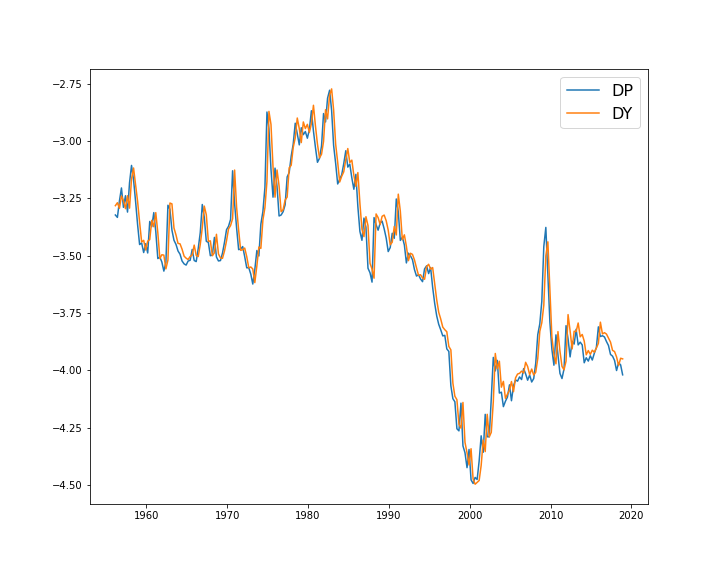
\includegraphics[width=1.2\linewidth]{co1.png}
			\caption{co1}
		\end{subfigure}
		\begin{subfigure}[b]{0.48\linewidth}
			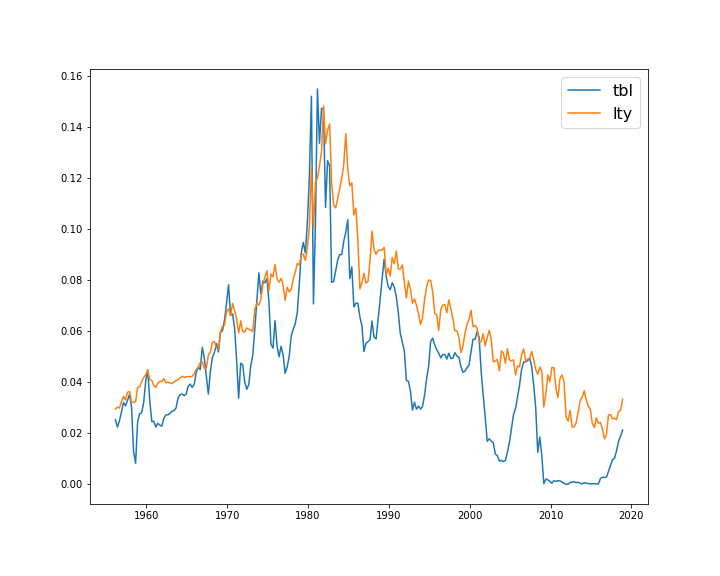
\includegraphics[width=1.2\linewidth]{co2.png}
			\caption{co2}
		\end{subfigure}
		\begin{subfigure}[b]{0.48\linewidth}
			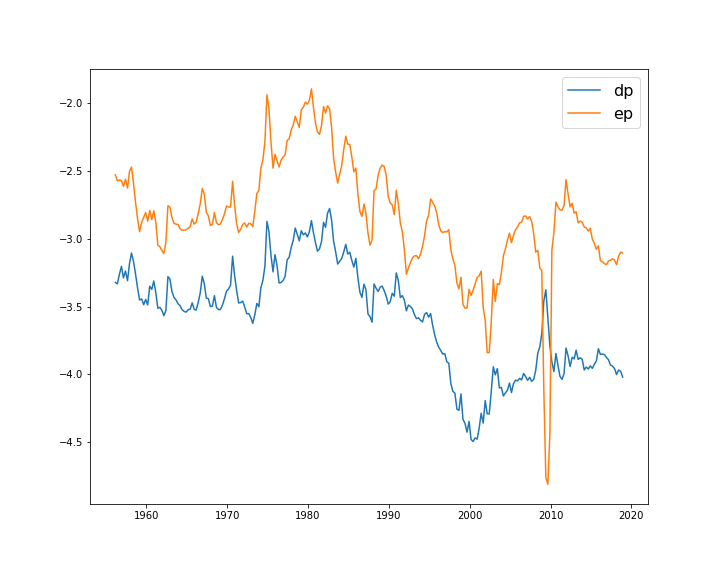
\includegraphics[width=1.2\linewidth]{co3.png}
			\caption{co3}
		\end{subfigure}
		\begin{subfigure}[b]{0.48\linewidth}
			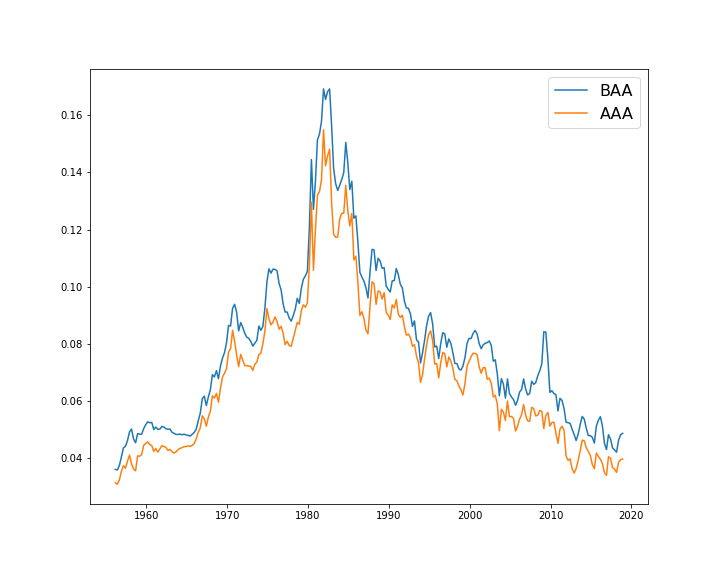
\includegraphics[width=1.2\linewidth]{co4.png}
			\caption{co4}
		\end{subfigure}
		\label{variables}
	\end{figure}
	
	Apart from the non-stationary variables, the partially nonlinear models also consider two stationary variables: the lagged stock return ($y_{t-1}$) and the regression residual from the study of \cite{lettau2001consumption}.
	In their study, they show that log consumption, log asset wealth and log labor income share a common stochastic trend and are co-integrated. The deviations from this shared trend is stationary and can be used as a predictor for stock return.
	
	Therefore in the partially nonlinear models we consider: 
	$$
	y_{t} = \beta_{1,0} y_{t-1} + \beta_{2,0} w_{t-1} + f\left( x_{t-1}^{\prime }\theta _{0},\gamma _{0}\right) +e_{t}, \quad
	e_{t}\sim i.i.d.N\left( 0,1\right) ,\ \ t=2,...,T,
	$$
	the dependent variable, $y_t$, is the equity premium defined as the S\&P500 value-weighted log excess returns. $y_{t-1}$ is the lagged equity premium, $x_{t-1}$ are the co-integrated variables from \cite{zhou2018semiparametric} and $w_{t-1}$ is the regression residual from \cite{lettau2001consumption}. 
	
	In terms of the nonlinear part $f\left( x_{t-1}^{\prime }\theta _{0},\gamma _{0}\right)$, we consider the following 7 commonly used nonlinear functions including trigonometric functions, exponential functions and polynomial functions. Then the partially nonlinear models in the empirical study can be written as:
	
	\begin{eqnarray*}
		\text{sin}: g_{1}\left( u_{t-1},\gamma _{0}\right) &=& \beta _{0} z_{t-1}^{\prime} + \sin \left( u_{t-1}+\gamma_{1,0}\right),  \\
		\text{cos}: g_{2}\left( u_{t-1},\gamma _{0}\right) &=& \beta _{0} z_{t-1}^{\prime} + \cos \left( u_{t-1}+\gamma_{1,0}\right), \\
		\text{scale\_dsin}: g_{3}\left( u_{t-1},\gamma_{0}\right) &=& \beta _{0} z_{t-1}^{\prime} + \sin \left( \gamma_{1,0}u_{t-1}+\gamma_{2,0}\right),  \\
		\text{scale\_cos}: g_{4}\left( u_{t-1},\gamma_{0}\right) &=& \beta _{0} z_{t-1}^{\prime} + \cos \left( \gamma_{1,0}u_{t-1}+\gamma_{2,0}\right), \\
		\text{exp\_shift}: g_{5}\left( u_{t-1}, \gamma_{0}\right) &=&  \beta _{0} z_{t-1}^{\prime} + 1-e^{-\gamma_{1,0}\left(u_{t-1}-\gamma_{2,0}\right)^{2}} \\
		\text{exp}: g_{6}\left( u_{t-1},\gamma _{0}\right) &=&  \beta _{0} z_{t-1}^{\prime} + \gamma_{1,0} e^{-\gamma_{2,0}u_{t-1}^2}  \\
		\text{Polynomial}: g_{7}\left( u_{t-1},\gamma_{0}\right) &=& \beta _{0} z_{t-1}^{\prime} + \gamma_{1,0}+ \gamma_{2,0}u_{t-1}+\gamma_{3,0}u_{t-1}^{2}
	\end{eqnarray*}%
	where $\beta_{0} = (\beta_{1,0}, \beta_{2,0})$, $ z_{t-1}^{\prime } = (y_{t-1}, w_{t-1})$, and $u_{t-1} =  x_{t-1}^{\prime }\theta _{0}$.
	
	% \noindent\textcolor{green}{\rule{16cm}{1mm}}
	
	In addition, we also include a linear functional form with single-index:
	$$
	\text{constrained\_linear}: g_8\left( u_{t-1}\right) = \gamma_{1,0} +\beta _{0} z_{t-1}^{\prime} + \gamma_{2,0}(x_{1,t-1}\theta _{1,0} + x_{2,t-1}\theta _{2,0}).
	$$
	As for other functional forms, in this constrained linear function, we set $\theta^2_{1,0}+\theta_{2,0}^2 = 1$ and use the same iterative procedure to estimate the model. 
	
	To estimate model $g_1$ to $g_7$, we adopt the constrained nonlinear least square method described in section (to be filled). But as mentioned before, when minimizing the nonlinear least squares:
	$$
	S_{T}(\beta, \theta, \gamma)=\sum_{t=1}^{T}\left(y_{t}-g\left(u_{t-1}, \gamma\right)\right)^{2}
	$$
	
	The gradient equations do not have a closed solution, so we use an iterative algorithm. To implement the iterative algorithm, we must choose a vector of initial values to start. Initial values can be specified by random number generation. One would generate many sets of initial values and then choose the one that leads to a better result. In our case, to better fit the data, we choose the initial values using linear regressions. The detailed steps are shown below:
	
	\textbf{Step 1}: estimate the following linear regression to get $\hat{\alpha}$:
	$$
	x_1 = \alpha x_2 + e_t, \quad e_{t}\sim i.i.d.N\left( 0,1\right) ,\ \ t=2,...,T
	$$
	where $x_1$ and $x_2$ are the non-stationary co-integrated variables. 
	Then, the initial values for $\theta$ is $\theta_{0} = (\dfrac{1}{\sqrt{1+\alpha^2}}, \dfrac{-\alpha}{\sqrt{1+\alpha^2}})$. 
	As $\theta_{0}$ is known, we can calculate $u_{t-1}$.
	
	\textbf{Step 2}: substitute the nonlinear function $f\left( u_{t-1},\gamma \right)$ by its Taylor expansion and estimate the following linear regression to obtain the initial values for $\beta$ and $\gamma$.
	
	\begin{eqnarray*}
		\text{sin}: \tilde{g_{1}}\left( u_{t-1},\gamma _{0}\right) &=& \left( \gamma_{1} + u_{t-1}\right) + \beta z_{t-1}^{\prime},  \\
		\text{cos}: \tilde{g_{2}}\left( u_{t-1},\gamma _{0}\right) &=& 1 - \left( \gamma_{1} + u_{t-1}\right)^2  + \beta z_{t-1}^{\prime}, \\
		\text{sin\_scaled}: \tilde{g_{3}}\left( u_{t-1},\gamma_{0}\right) &=& \gamma_{2}  + \gamma_{1}u_{t-1} + \beta z_{t-1}^{\prime},  \\
		\text{cos\_scaled}: \tilde{g_{4}}\left( u_{t-1},\gamma_{0}\right) &=& 1 - \left( \gamma_{2} + \gamma_{1}u_{t-1}\right)^2  + \beta z_{t-1}^{\prime}, \\
		\text{exp\_shift}: \tilde{g_{5}}\left( u_{t-1}, \gamma_{0}\right) &=&  \gamma_{1,0}u_{t-1}^2 - 2\gamma_{1,0}\gamma_{2,0}u_{t-1} + \gamma_{1,0}\gamma_{2,0}^2 + \beta z_{t-1}^{\prime} \\
		\text{exp}: \tilde{g_{6}}\left( u_{t-1},\gamma _{0}\right) &=&  \gamma_{1,0}(1-\gamma_{2,0}u_{t-1}^2 + \dfrac{\gamma_{2,0}^2 u_{t-1}^4}{2}) + \beta z_{t-1}^{\prime}, \\
		\text{Polynomial}: \tilde{g_{7}}\left( u_{t-1},\gamma_{0}\right) &=& \gamma_{1}+ \gamma_{2}u_{t-1}+\gamma_{3}u_{t-1}^{2}+\beta z_{t-1}^{\prime}, \\
		\text{constrained\_linear}: \tilde{g_{8}}\left( u_{t-1},\gamma_{0}\right) &=& \gamma_{1}+ \gamma_{2}u_{t-1}+\beta z_{t-1}^{\prime}
	\end{eqnarray*}%
	where $\beta = (\beta_{1}, \beta_{2})$, $ z_{t-1}^{\prime } = (y_{t-1}, w_{t-1})$, and $u_{t-1}$ has been calculated in step 1 above.
	
	In the simulation section, we have shown that by using Taylor-initials, the convergence of the estimators have improved significantly. In this section, we will investigate the empirical performances of our partially nonlinear models using the Taylor-initials.
	
	% \noindent\textcolor{green}{\rule{16cm}{1mm}}
	
	% Following \cite{welch2008comprehensive}, we use the sample mean model as a benchmark. The sample mean model can be defined as:
	
	% $$
	% y_t= \dfrac{1}{t-1}\sum_{1}^{t-1}y_i
	% $$
	
	% \noindent\textcolor{green}{\rule{16cm}{1mm}}
	
	
	% In addition, we also adopt auto-regressive models as additional benchmarks for comparison. We consider 3 forms of AR models: AR(1) model, AR(2) model, and an AR(1) model with the cay variable.
	% \begin{itemize}
	% 	\item AR1:
	% 	$$
	% 	y_t = \beta_{1}y_{t-1} + \epsilon_t
	% 	$$
	% 	\item AR2:
	% 	$$
	% 	y_t =\beta_{1,0} y_{t-1} + \beta_{2,0} y_{t-2} + \epsilon_t
	% 	$$
	% 	\item AR1 model with "cay" variable (AR\_cay):
	% 	$$
	% 	y_t = \beta_{1,0}y_{t-1} + \beta_{2,0}cay_{t-1} + \epsilon_t
	% 	$$
	% \end{itemize}
	
	% We also include a nonlinear model which has the same nonlinear part as in the partially nonlinear model, but does not include the lagged dependent variable and the "cay" variable.
	% \begin{itemize}
	% 	\item Nonlinear single-index model (NLS):
	% 	$$
	% 	y_{t} = f\left( x_{t-1}^{\prime }\theta _{0},\beta _{0}\right) + \epsilon_{t},
	% 	$$
	% \end{itemize}
	% where $\epsilon_{t}\sim i.i.d.N\left( 0,1\right)$ for all the benchmark models.
	
	\subsection{In-sample Results}
	In this section, we use the complete sample from 1956 Q1 to 2018 Q4 to investigate the in-sample performances of our partially nonlinear models. We define the in-sample $R^2_{IS}$ as a measurement for the in-sample performance:
	\begin{equation}
		R_{IS}^{2}=1-\frac{\sum_{t=1}^{n}\left(y_{t}-\widehat{y}_{t}\right)^{2}}{\sum_{t=1}^{n}\left(y_{t}-\bar{y}\right)^{2}}
	\end{equation}
	where $y_t$ is the observed stock return in time t, $\bar{y}$ is the predicted return from the benchmark model, and $\hat{y_{t}}$ is the corresponding predicted stock return. 
	
	% The sample mean model can be defined as:
	% $$
	% \bar{y_t}= \dfrac{1}{t-1}\sum_{1}^{t-1}y_i.
	% $$
	
	$R^2_{IS}$ can also be rewritten as:
	\begin{equation}
		R_{IS}^{2}=1-\frac{MSE_{CLS}}{MSE_{bm}}
		\label{Ris}
	\end{equation}
	where $MSE_{bm}$ is the mean squared error of benchmark model and $\mathrm{MSE}_{CLS}=1 / n \sum_{t=1}^{n}\left(y_{t}-\hat{y_t}\right)^{2}$ is the mean squared error of our partially nonlinear models. 
	In the study of \cite{welch2008comprehensive}, they found that sample mean is a competitive model in stock return prediction. Therefore, we use the sample mean model as the benchmark. 
	% And $MSE_{bm}$ in (\ref{Ris}) is $\mathrm{MSE}_{bm}=1 / n \sum_{t=1}^{n}\left(y_{t}-\bar{y}\right)^{2}$.
	
	In equation (\ref{Ris}), if $R^2_{IS}$ for a given model is positive, it indicates that the model outperforms the benchmark model, and the bigger the value is, the better the corresponding model performs.
	
	The results of $R^2_{IS}$ is reported in table \ref{ins_R2}. Among the 8 functional forms, $g_3$, $g_4$, $g_5$, $g_7$ and $g_8$ provide positive $R^2_{IS}$ for all 4 variable combinations, which means the 5 functional forms have better in-sample performances than historical benchmark. And for $g_1$, $g_2$ and $g_6$, they can outperform sample mean model for some of the variable combinations. 
	
	
	% and we find that for all the variable combinations, we can find at least one partially nonlinear model that can outperform sample mean model. 
	% In addition, functional 3, 4, 7 and 8 show positive in-sample performances for all the combinations.
	
	\begin{table}[!htbp]
		\centering
		\caption{Results of $R^2_{IS}$ for all the models (benchmark: sample mean model)}
		\begin{adjustbox}{max width=\textwidth}
			\begin{tabular}{ccccccccc}
				\toprule
				\textbf{variables} & \textbf{function} & \textbf{$R^2_{IS}$} & \textbf{function} & \textbf{$R^2_{IS}$} & \textbf{function} & \textbf{$R^2_{IS}$} & \textbf{function} & \textbf{$R^2_{IS}$} \\
				\midrule
				\textbf{co1} & \multirow{4}[1]{*}{\textbf{$g_1$}} & -0.37483 & \multirow{4}[1]{*}{\textbf{$g_3$}} & 0.00656 & \multirow{4}[1]{*}{\textbf{$g_5$}} & 0.02287 & \multirow{4}[1]{*}{\textbf{$g_7$}} & 0.01445 \\
				\textbf{co2} &       & 0.01603 &       & 0.01633 &       & 0.00000 &       & 0.01626 \\
				\textbf{co3} &       & -5.82166 &       & 0.00115 &       & 0.02376 &       & 0.01814 \\
				\textbf{co4} &       & -0.00622 &       & 0.01026 &       & 0.00000 &       & 0.01493 \\
				\midrule
				\textbf{co1} & \multirow{4}[1]{*}{\textbf{$g_2$}} & -0.57967 & \multirow{4}[1]{*}{\textbf{$g_4$}} & 0.01183 & \multirow{4}[1]{*}{\textbf{$g_6$}} & -0.07239 & \multirow{4}[1]{*}{\textbf{$g_8$}} & 0.00780 \\
				\textbf{co2} &       & -0.03409 &       & 0.01633 &       & -0.02301 &       & 0.01633 \\
				\textbf{co3} &       & -5.50946 &       & 0.00618 &       & 0.01751 &       & 0.00077 \\
				\textbf{co4} &       & 0.00615 &       & 0.01026 &       & -0.02565 &       & 0.01025 \\
				\bottomrule
				\bottomrule
			\end{tabular}%
		\end{adjustbox}
		\label{ins_R2}%
	\end{table}%
	
	
	\subsection{OOS Results}
	Since the existing literatures show that the evidence for stock return predictability only hold for in-sample, in this section, we investigate how our models perform out-of-sample. Following \cite{campbell2008predicting}, we use the OOS $R^2$ to measure the forecasting performance. The $R^2_{OOS}$ is defined as:
	
	\begin{equation}
		R_{O O S, j, n, R}^{2}=1-\frac{\sum_{r=1}^{R}\left(y_{n+r, j}-\widehat{y}_{n+r, j}\right)^{2}}{\sum_{r=1}^{R}\left(y_{n+r, j}-\bar{y}_{n+r, j}\right)^{2}}
		\label{Rdef}
	\end{equation}
	where n is the sample size of initial data to get a regression estimate at the start of evaluation period, R is the total number of expansive windows. In our case, n = 128 (from 1956 Q1 to 1987 Q4) and the maxmum of R is 124 (from 1988 Q1 to 2018 Q4). We also set j = 1 because we only consider 1-step forecast. To make the notation simpler, we will ignore the subscript j in the rest of the chapter.  
	
	In the above definition, $\hat{y}_{n+r}$ is the 1-step predicted return in the r-th window. $\bar{y}_{n+r}$ is the sample mean of observations using the information up to $n+r-1$,  $y_{n+r}$ is the observed return in period $n+r$. 
	
	To generate the first out-of-sample stock return forecast, we use the first n-1 pairs of observations \{($x_1$, $y_2$), ($x_2$, $y_3$), $\cdots$, ($x_{n-1}$, $y_{n}$)\} to estimate the nonlinear model and predict $\hat{y}_{n+1}$ and $\bar{y}_{n+1}$. 
	We then include the information in the $n+1$ period and predict $\hat{y}_{n+2}$ and $\bar{y}_{n+2}$ using \{($x_1$, $y_2$), ($x_2$, $y_3$), $\cdots$, ($x_{n}$, $y_{n+1}$)\}. 
	The procedure continues until we obtain $\hat{y}_{n+R}$ and $\bar{y}_{n+R}$. The predicted values are denoted by:
	\begin{center}
		$\hat{y}_{n+1}$, $\hat{y}_{n+2}$, $\cdots$, $\hat{y}_{n+R}$
		
		$\bar{y}_{n+1}$, $\bar{y}_{n+2}$, $\cdots$, $\bar{y}_{n+R}$
	\end{center}
	
	Using these predicted values, we can calculate the $R_{O O S, j, n, R}^{2}$ using the definition (\ref{Rdef}). To show how the out-of-sample forecasting performance when the forecasting window is expanding, we look at the cumulative out-of-sample $R^2$.
	
	Cumulative $R_{O O S, n, R}^{2}$ can be obtained with R ranging from 1 to 124 (in our previous chapter). In \cite{cheng2019nonparametric}, they use $R^2_{OOS}$ starting from R = 12 (1 year, 12 months). Therefore in this chapter, I will follow their choice of $R^2_{OOS}$ and start from R = 4 (1 year, 4 quarters). 
	
	The OOS results for different functional forms are shown in the following figures. We report out-of-sample results in
	8 figures, each of which shows the prediction of different functional forms using the 4 co-integrated combinations. We put the $R^2_{OOS}$ statistics on the vertical axis and the beginning of the various out-of-sample evaluation periods on the horizontal axis. 
	
	Figure (\ref{g1}) and (\ref{g2}) show the performances of the two trigonometric functions compared with sample mean. They have similar OOS performance for each of the 4 variable pairs and we can only find positive results for combinations co2 (tbl and lty) and co4 (baa or aaa-rated bonds). But from the sub-figure (d), we can see that function $g_1$ is better than $g_2$ since it provide consecutive positive $R^2_{OOS}$ from 1996 to 2012.
	
	Figure (\ref{g3}) and (\ref{g4}) display results for the scaled trigonometric functions $g_3$ and $g_4$. These two functions are different from $g_1$ and $g_2$ in that they have a scale parameter in front of the single-index while $g_1$ and $g_2$ do not. 
	Similar to the trigonometric functions, $g_3$ and $g_4$ only show positive $R^2_{OOS}$ for combinations co2 (lty and tbl) and co4 (baa or aaa-rated bonds), and the results are almost identical for the 4 variable combinations except for co4 , where $g_3$ have a better forecast.
	
	The results for the two exponential functions are presented in figure (\ref{g5}) and (\ref{g6}). For functional $g_5$, it cannot outperform sample mean model for most of the out-of-sample forecasting period. We can only find a positive spike around 1992 for co1 (dp and dy),  (lty and tbl) and co4 (baa or aaa-rated bonds). 
	
	For functional $g_6$, the positive $R^2_{OOS}$ can be found in the first half of the forecasting period. We can see from sub-figures (b) and (d) of figure (\ref{g6}) that $g_6$ gives consecutive positive results before 2014 when using combinations co2 and co4. 
	
	Figure (\ref{g7}) presents the forecasting results of the polynomial function $g_7$. Positive $R^2_{OOS}$ can be found for combinations co2 and co4 before 2014. Forecasting results of $g_8$ in figure (\ref{g8}) are similar to $g_7$ for combinations co1, co2 and co3. Although the results of co4 is different, the positive values are only present in the first half of the forecasting period. 
	
	
	\begin{figure}[!htbp]
		\centering
		\caption{OOS Results for Model with $f_1$}
		\begin{subfigure}[b]{0.42\linewidth}
			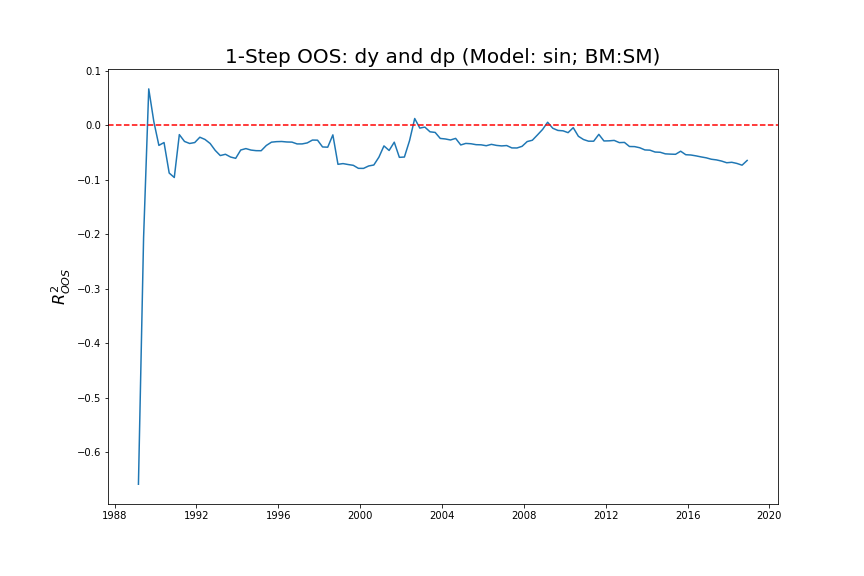
\includegraphics[width=0.9\linewidth]{OOS_plots/sin_co1_SM.png}
			\caption{co1}
		\end{subfigure}
		\begin{subfigure}[b]{0.42\linewidth}
			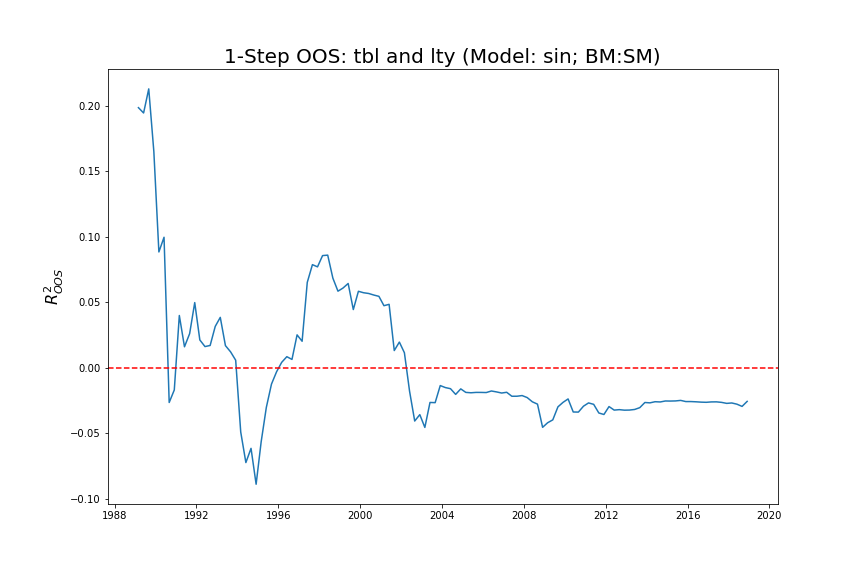
\includegraphics[width=0.9\linewidth]{OOS_plots/sin_co2_SM.png}
			\caption{co2}
		\end{subfigure}
		\begin{subfigure}[b]{0.42\linewidth}
			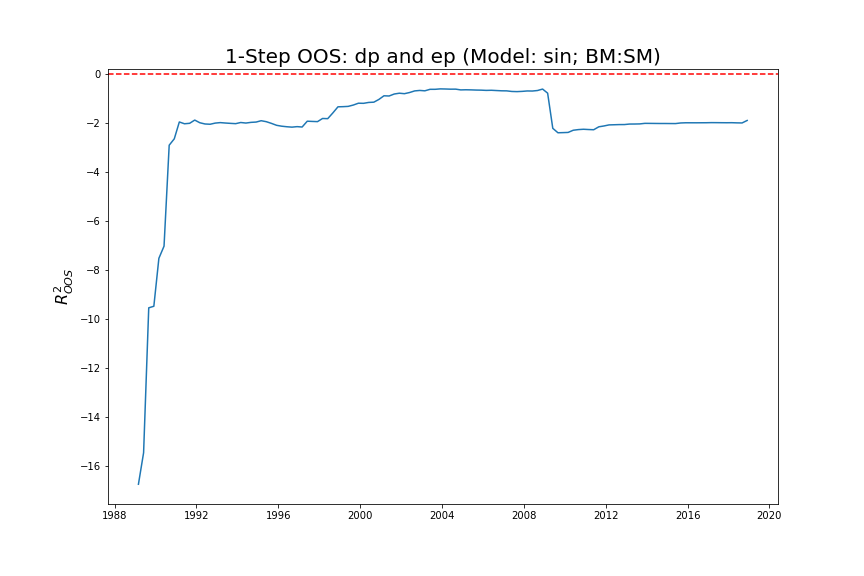
\includegraphics[width=0.9\linewidth]{OOS_plots/sin_co3_SM.png}
			\caption{co3}
		\end{subfigure}
		\begin{subfigure}[b]{0.42\linewidth}
			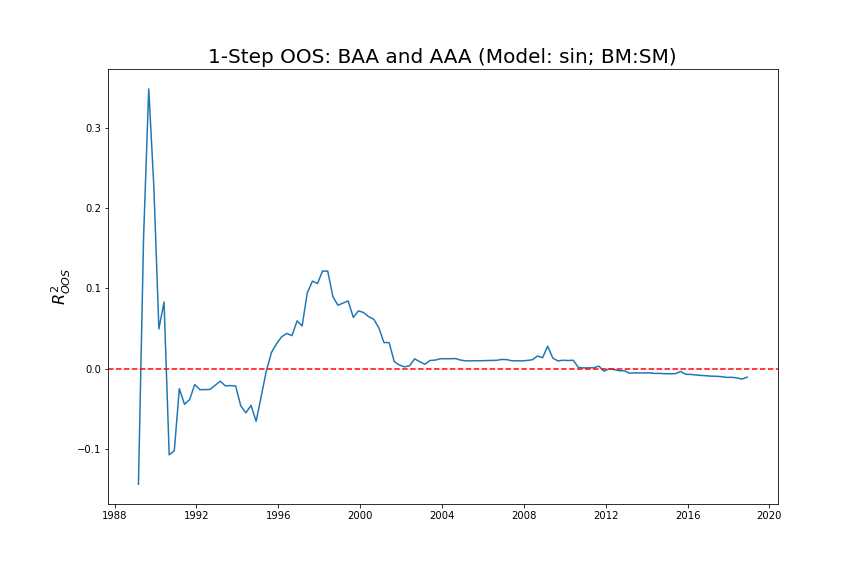
\includegraphics[width=0.9\linewidth]{OOS_plots/sin_co4_SM.png}
			\caption{co4}
		\end{subfigure}
		\label{g1}
	\end{figure}
	
	\begin{figure}[!htbp]
		\centering
		\caption{OOS Results for Model with $f_2$}
		\begin{subfigure}[b]{0.42\linewidth}
			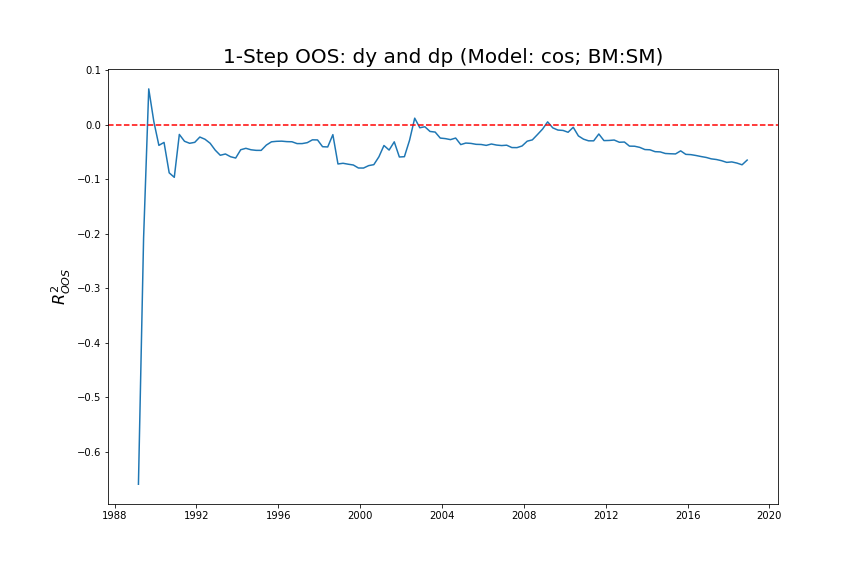
\includegraphics[width=0.9\linewidth]{OOS_plots/cos_co1_SM.png}
			\caption{co1}
		\end{subfigure}
		\begin{subfigure}[b]{0.42\linewidth}
			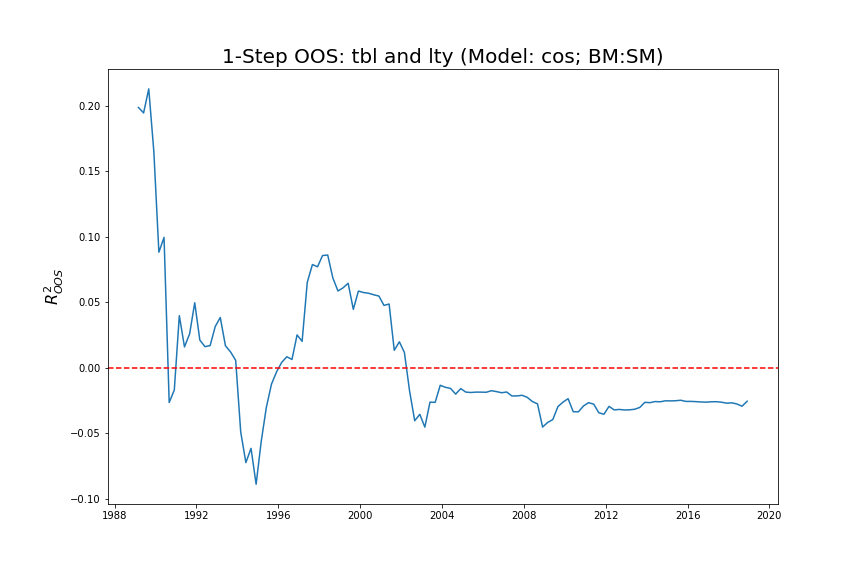
\includegraphics[width=0.9\linewidth]{OOS_plots/cos_co2_SM.png}
			\caption{co2}
		\end{subfigure}
		\begin{subfigure}[b]{0.42\linewidth}
			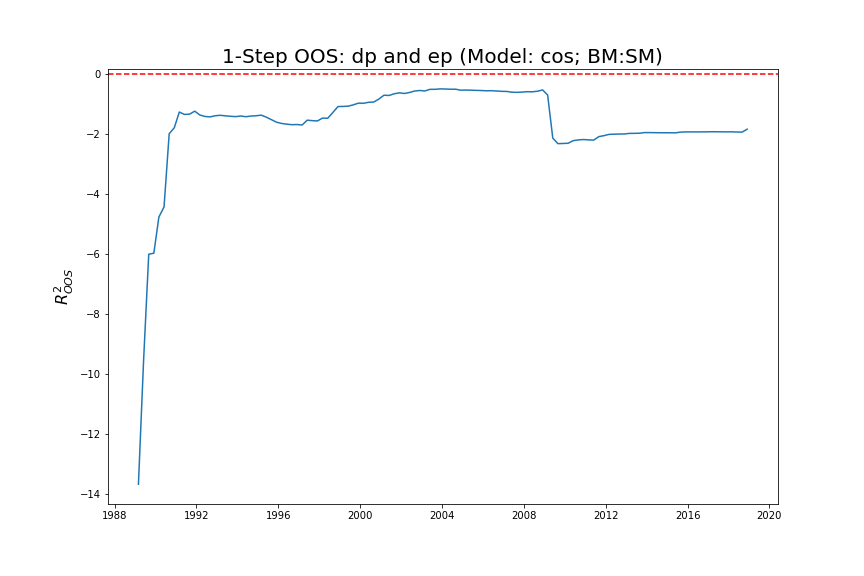
\includegraphics[width=0.9\linewidth]{OOS_plots/cos_co3_SM.png}
			\caption{co3}
		\end{subfigure}
		\begin{subfigure}[b]{0.42\linewidth}
			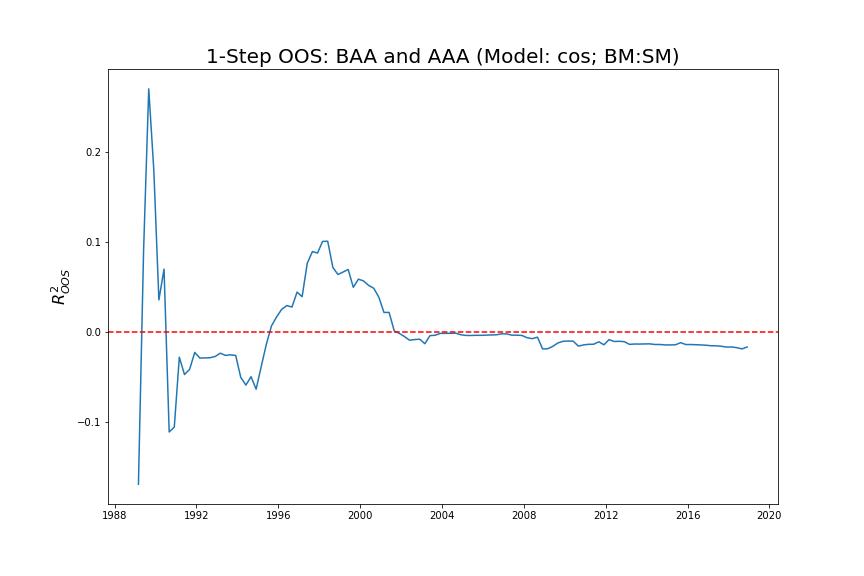
\includegraphics[width=0.9\linewidth]{OOS_plots/cos_co4_SM.png}
			\caption{co4}
		\end{subfigure}
		\label{g2}
	\end{figure}
	
	\begin{figure}[!htbp]
		\centering
		\caption{OOS Results for Model with $f_3$}
		\begin{subfigure}[b]{0.42\linewidth}
			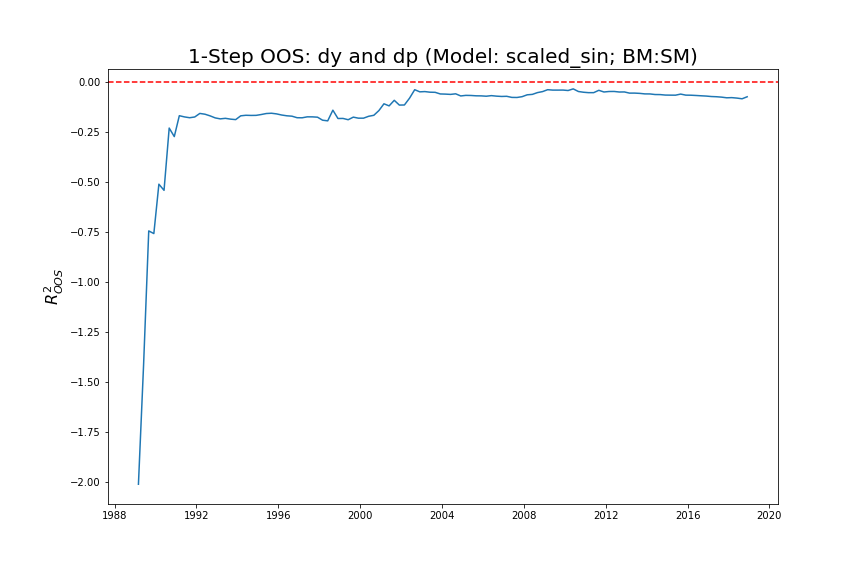
\includegraphics[width=0.9\linewidth]{OOS_plots/scaled_sin_co1_SM.png}
			\caption{co1}
		\end{subfigure}
		\begin{subfigure}[b]{0.42\linewidth}
			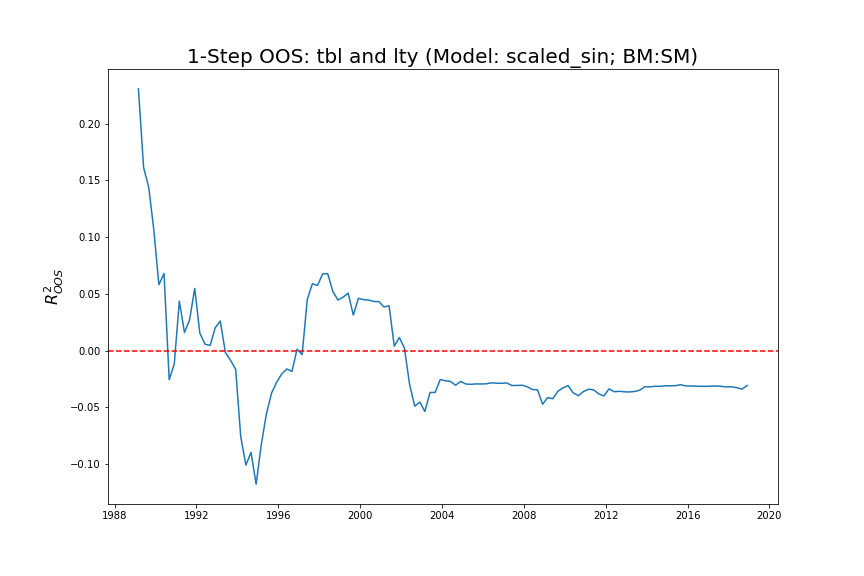
\includegraphics[width=0.9\linewidth]{OOS_plots/scaled_sin_co2_SM.png}
			\caption{co2}
		\end{subfigure}
		\begin{subfigure}[b]{0.42\linewidth}
			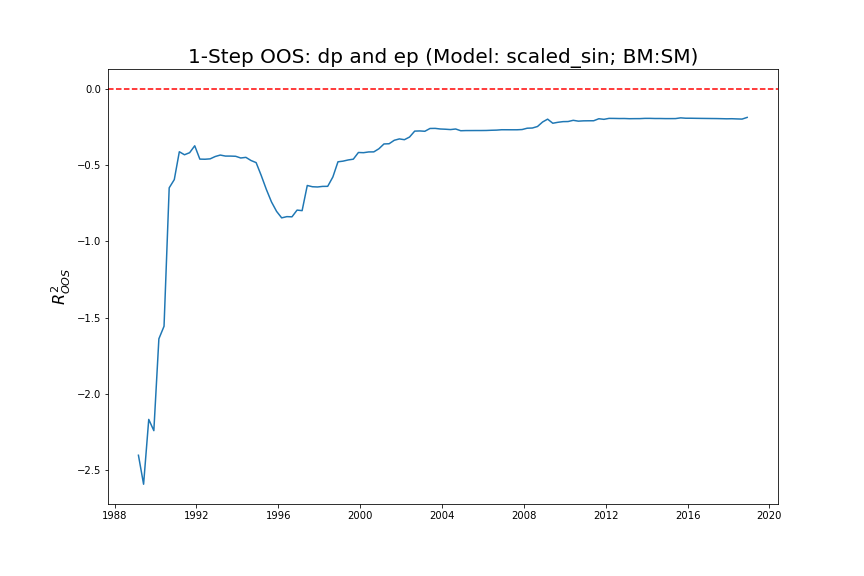
\includegraphics[width=0.9\linewidth]{OOS_plots/scaled_sin_co3_SM.png}
			\caption{co3}
		\end{subfigure}
		\begin{subfigure}[b]{0.42\linewidth}
			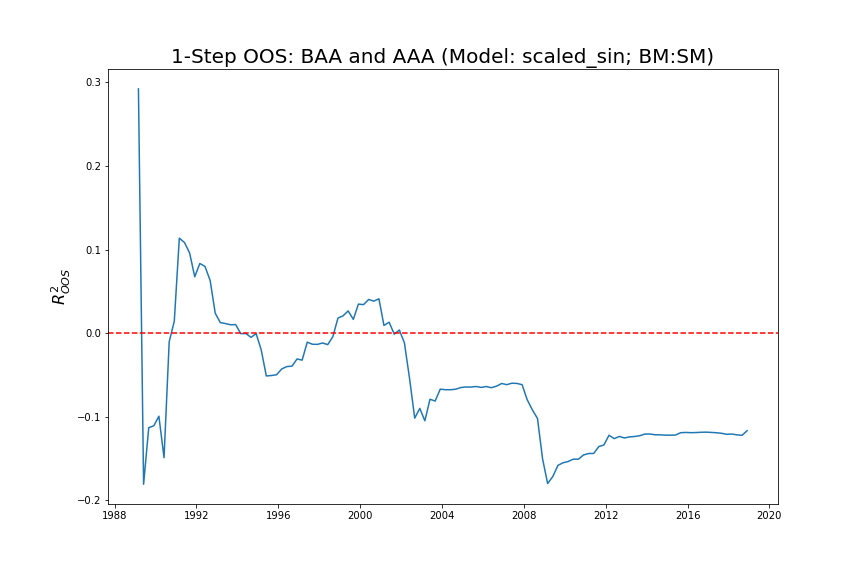
\includegraphics[width=0.9\linewidth]{OOS_plots/scaled_sin_co4_SM.png}
			\caption{co4}
		\end{subfigure}
		\label{g3}
	\end{figure}
	
	\begin{figure}[!htbp]
		\centering
		\caption{OOS Results for Model with $f_4$}
		\begin{subfigure}[b]{0.42\linewidth}
			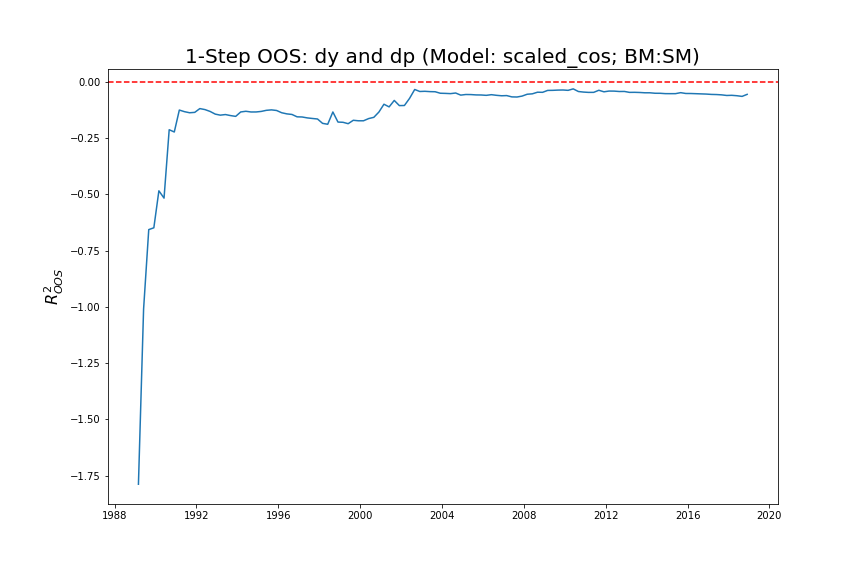
\includegraphics[width=0.9\linewidth]{OOS_plots/scaled_cos_co1_SM.png}
			\caption{co1}
		\end{subfigure}
		\begin{subfigure}[b]{0.42\linewidth}
			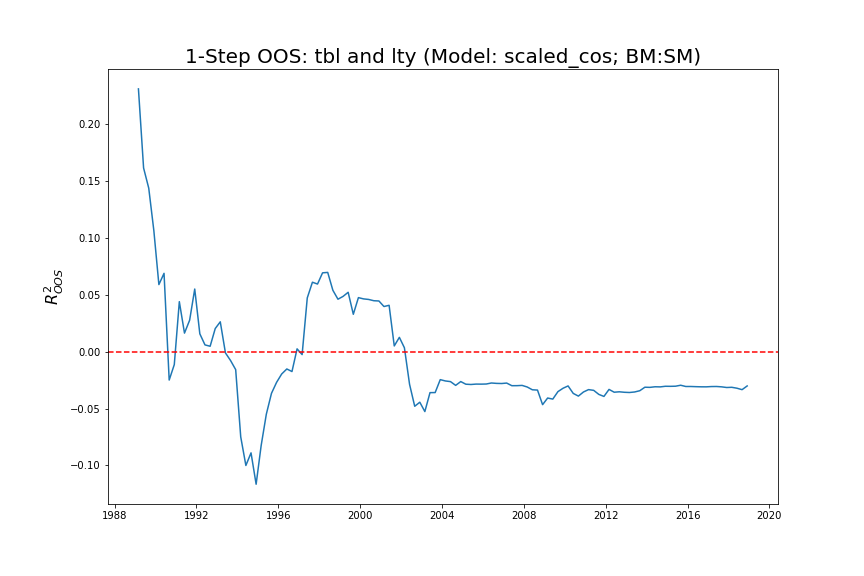
\includegraphics[width=0.9\linewidth]{OOS_plots/scaled_cos_co2_SM.png}
			\caption{co2}
		\end{subfigure}
		\begin{subfigure}[b]{0.42\linewidth}
			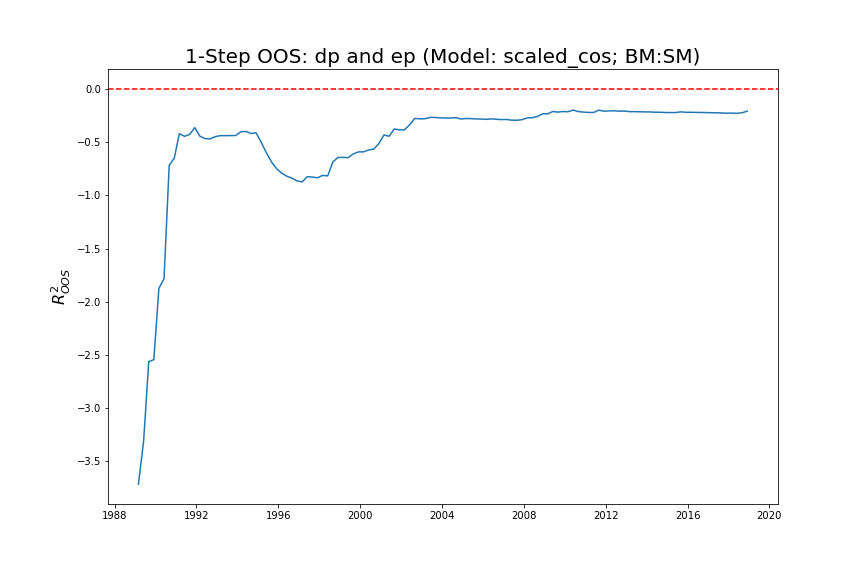
\includegraphics[width=0.9\linewidth]{OOS_plots/scaled_cos_co3_SM.png}
			\caption{co3}
		\end{subfigure}
		\begin{subfigure}[b]{0.42\linewidth}
			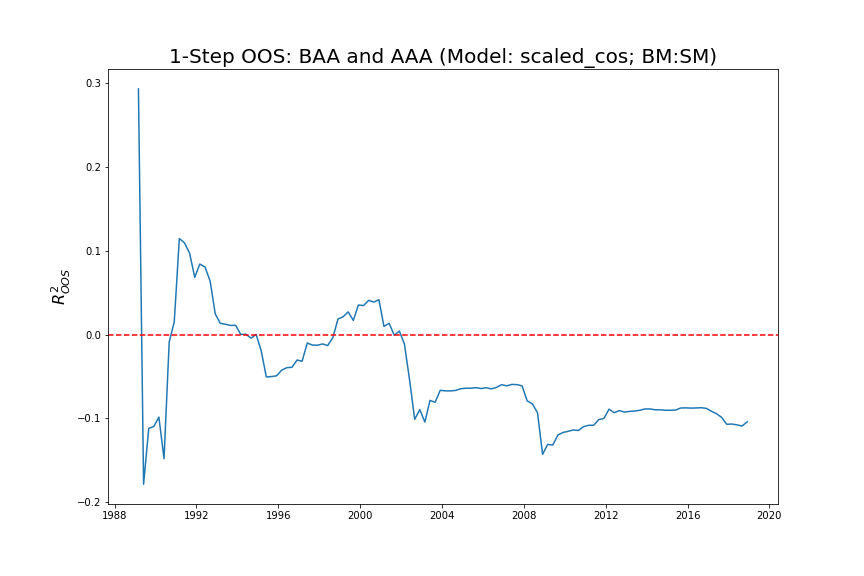
\includegraphics[width=0.9\linewidth]{OOS_plots/scaled_cos_co4_SM.png}
			\caption{co4}
		\end{subfigure}
		\label{g4}
	\end{figure}
	
	
	\begin{figure}[!htbp]
		\centering
		\caption{OOS Results for Model with $f_5$}
		\begin{subfigure}[b]{0.42\linewidth}
			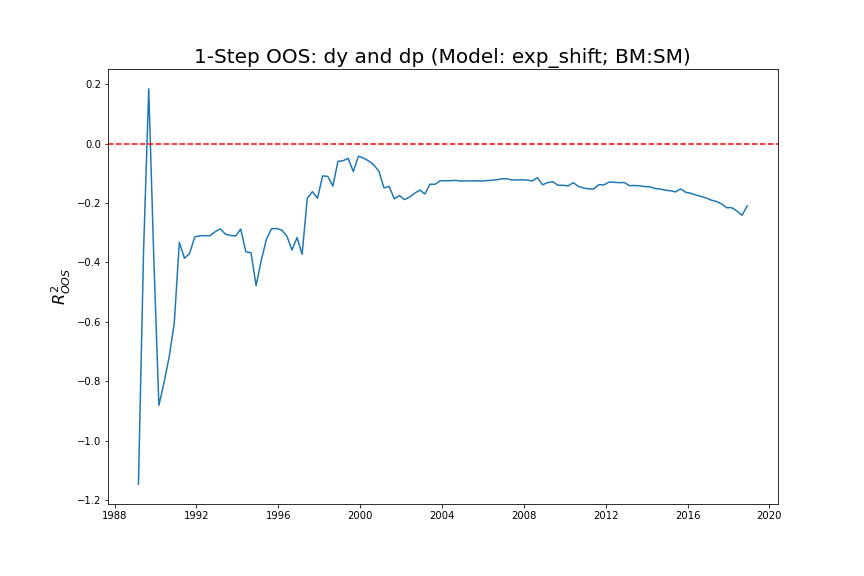
\includegraphics[width=0.9\linewidth]{OOS_plots/exp_shift_co1_SM.png}
			\caption{co1}
		\end{subfigure}
		\begin{subfigure}[b]{0.42\linewidth}
			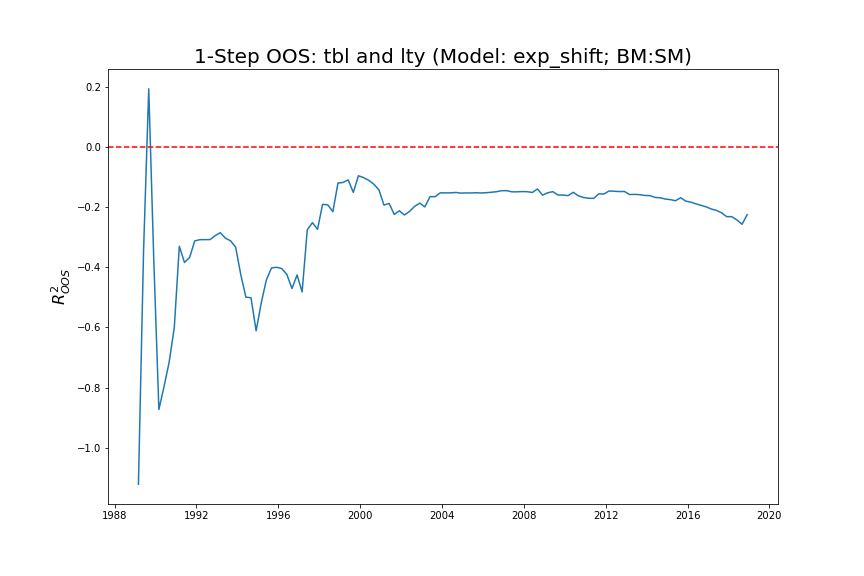
\includegraphics[width=0.9\linewidth]{OOS_plots/exp_shift_co2_SM.png}
			\caption{co2}
		\end{subfigure}
		\begin{subfigure}[b]{0.42\linewidth}
			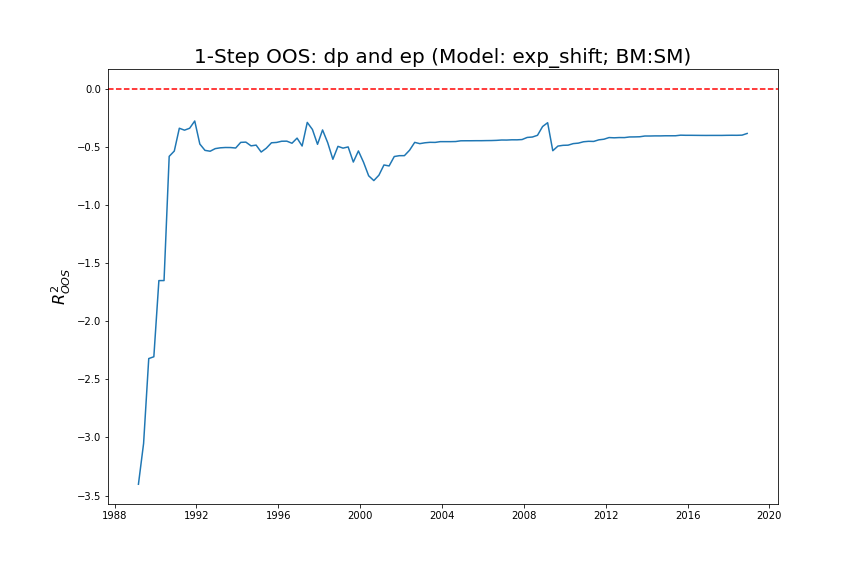
\includegraphics[width=0.9\linewidth]{OOS_plots/exp_shift_co3_SM.png}
			\caption{co3}
		\end{subfigure}
		\begin{subfigure}[b]{0.42\linewidth}
			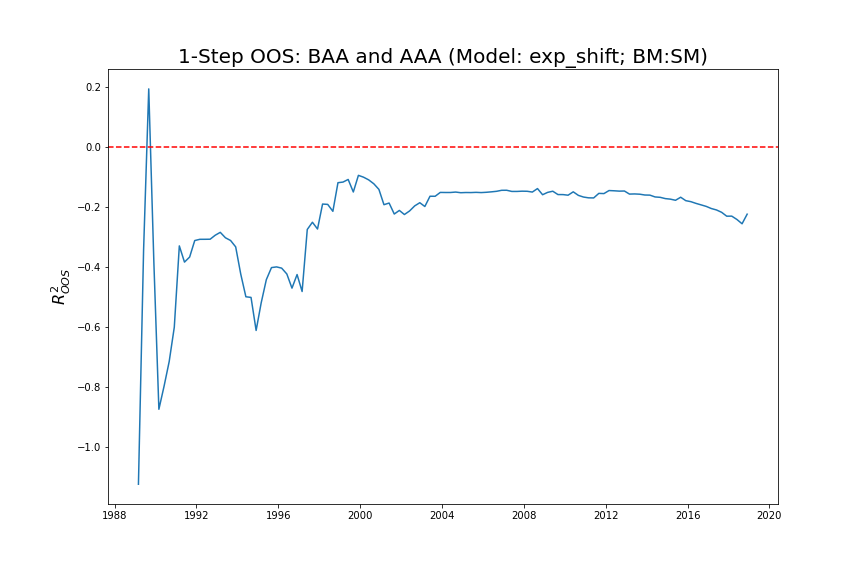
\includegraphics[width=0.9\linewidth]{OOS_plots/exp_shift_co4_SM.png}
			\caption{co4}
		\end{subfigure}
		\label{g5}
	\end{figure}
	
	\begin{figure}[!htbp]
		\centering
		\caption{OOS Results for Model with $f_6$}
		\begin{subfigure}[b]{0.42\linewidth}
			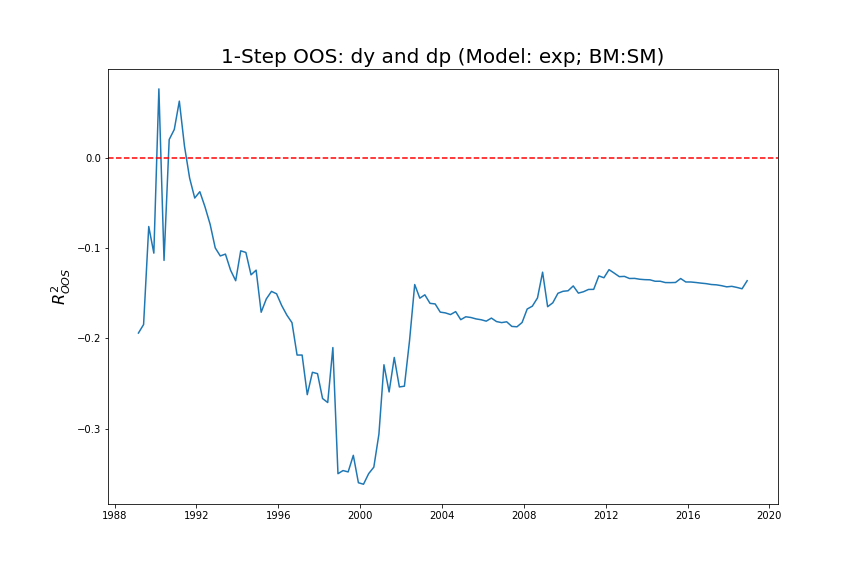
\includegraphics[width=0.9\linewidth]{OOS_plots/exp_co1_SM.png}
			\caption{co1}
		\end{subfigure}
		\begin{subfigure}[b]{0.42\linewidth}
			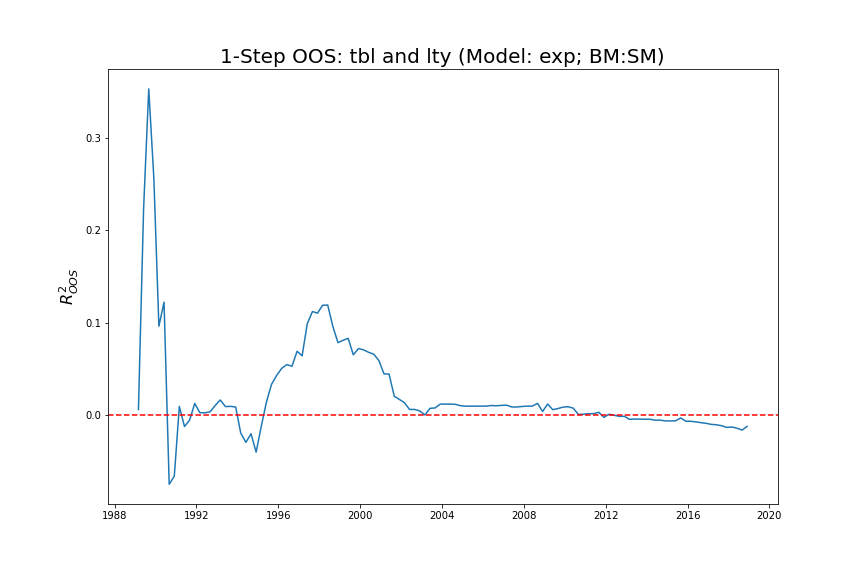
\includegraphics[width=0.9\linewidth]{OOS_plots/exp_co2_SM.png}
			\caption{co2}
		\end{subfigure}
		\begin{subfigure}[b]{0.42\linewidth}
			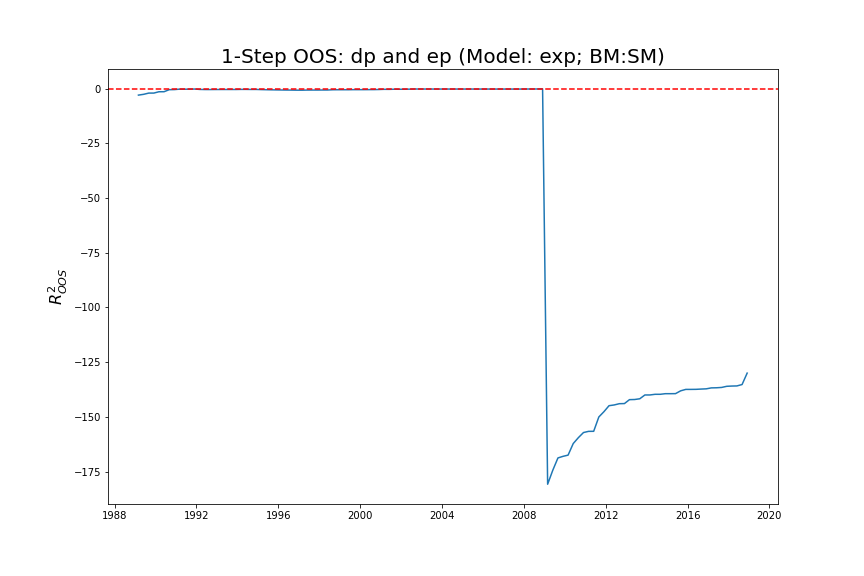
\includegraphics[width=0.9\linewidth]{OOS_plots/exp_co3_SM.png}
			\caption{co3}
		\end{subfigure}
		\begin{subfigure}[b]{0.42\linewidth}
			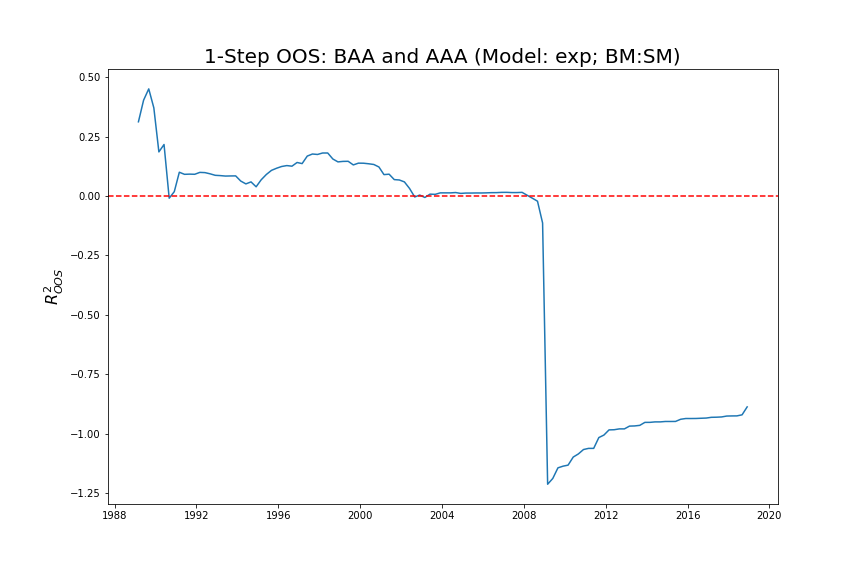
\includegraphics[width=0.9\linewidth]{OOS_plots/exp_co4_SM.png}
			\caption{co4}
		\end{subfigure}
		\label{g6}
	\end{figure}
	
	
	\begin{figure}[!htbp]
		\centering
		\caption{OOS Results for Model with $f_7$}
		\begin{subfigure}[b]{0.42\linewidth}
			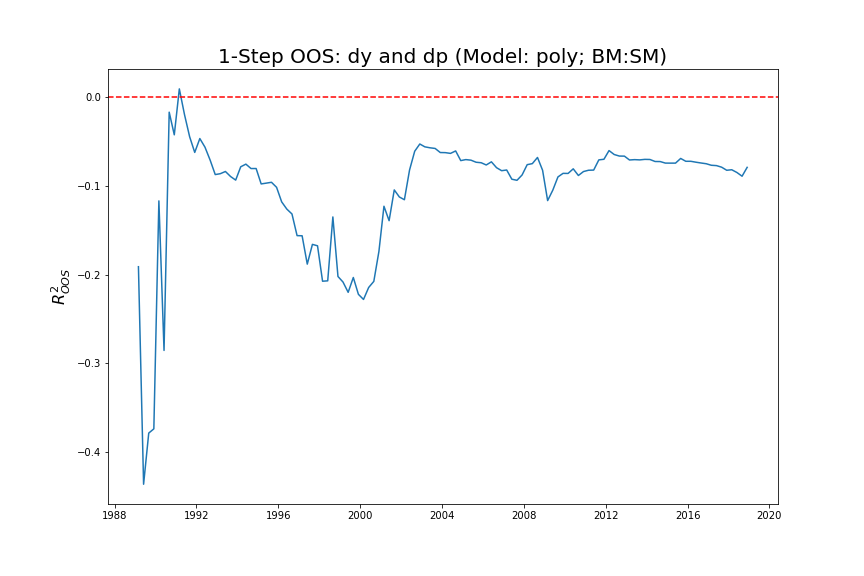
\includegraphics[width=0.9\linewidth]{OOS_plots/poly_co1_SM.png}
			\caption{co1}
		\end{subfigure}
		\begin{subfigure}[b]{0.42\linewidth}
			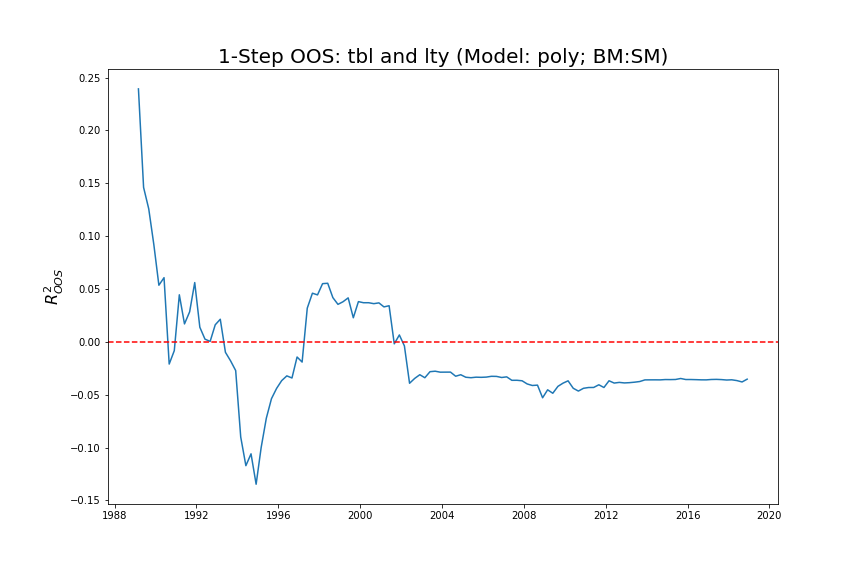
\includegraphics[width=0.9\linewidth]{OOS_plots/poly_co2_SM.png}
			\caption{co2}
		\end{subfigure}
		\begin{subfigure}[b]{0.42\linewidth}
			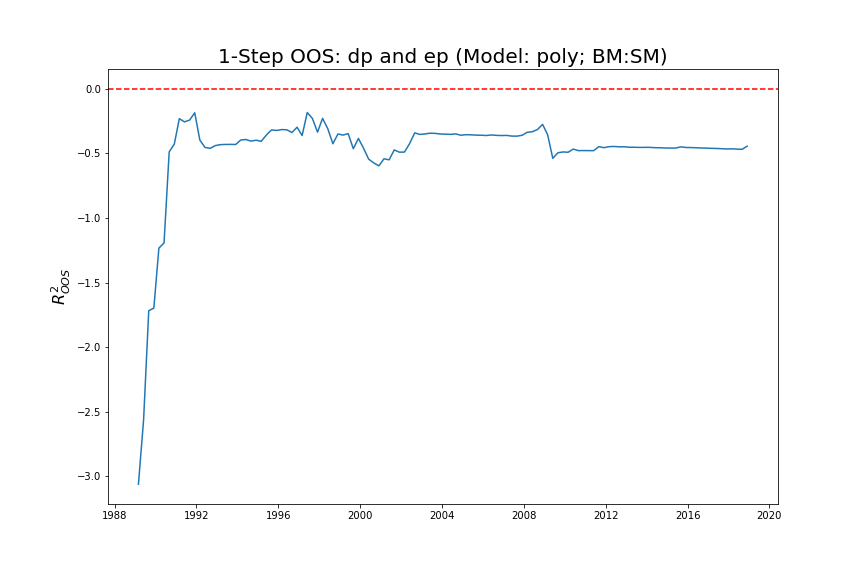
\includegraphics[width=0.9\linewidth]{OOS_plots/poly_co3_SM.png}
			\caption{co3}
		\end{subfigure}
		\begin{subfigure}[b]{0.42\linewidth}
			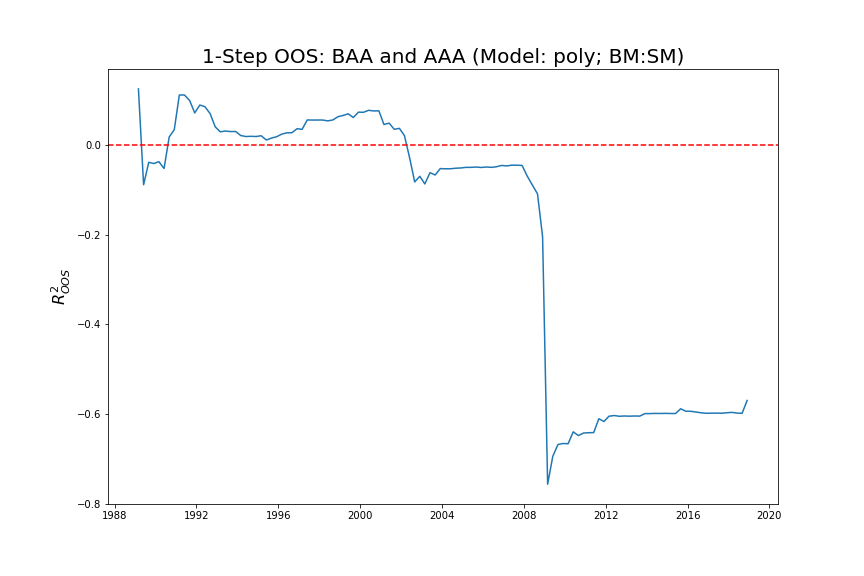
\includegraphics[width=0.9\linewidth]{OOS_plots/poly_co4_SM.png}
			\caption{co4}
		\end{subfigure}
		\label{g7}
	\end{figure}
	
	\begin{figure}[!htbp]
		\centering
		\caption{OOS Results for Model with $g_8$}
		\begin{subfigure}[b]{0.42\linewidth}
			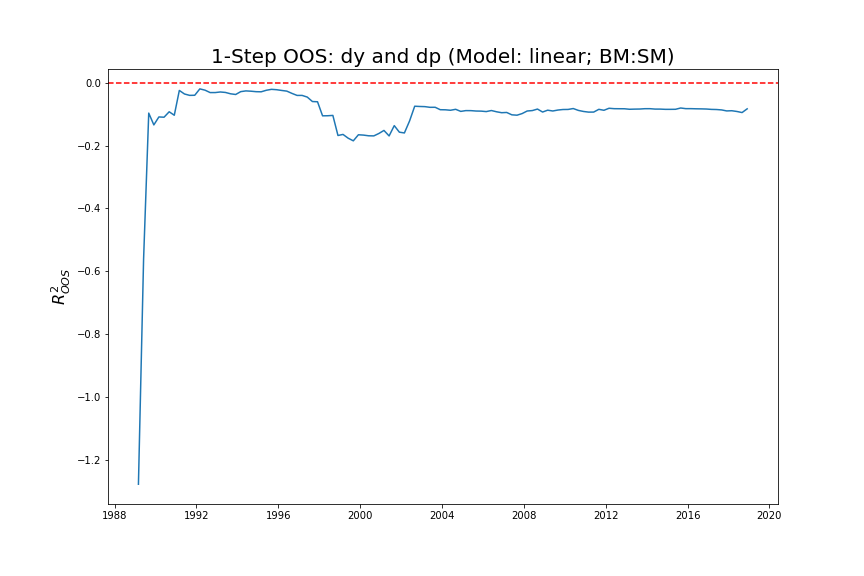
\includegraphics[width=0.9\linewidth]{OOS_plots/linear_co1_SM.png}
			\caption{co1}
		\end{subfigure}
		\begin{subfigure}[b]{0.42\linewidth}
			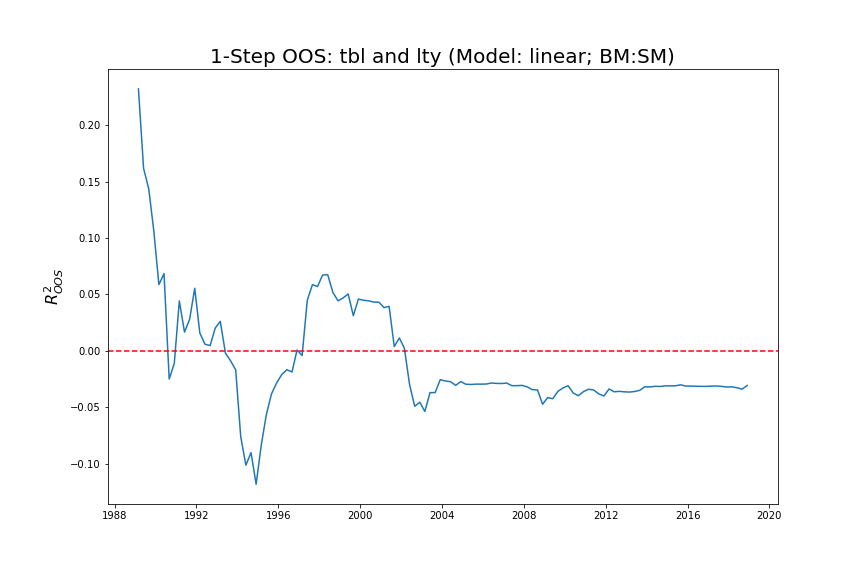
\includegraphics[width=0.9\linewidth]{OOS_plots/linear_co2_SM.png}
			\caption{co2}
		\end{subfigure}
		\begin{subfigure}[b]{0.42\linewidth}
			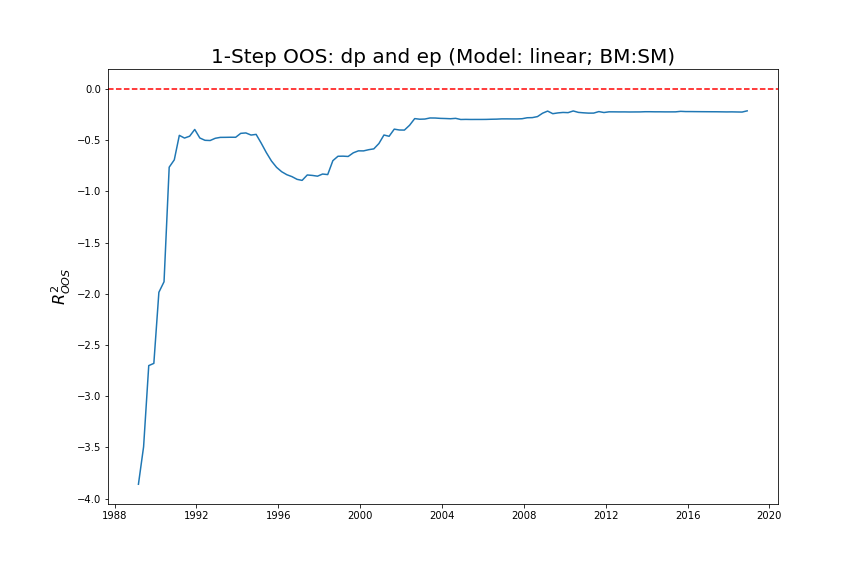
\includegraphics[width=0.9\linewidth]{OOS_plots/linear_co3_SM.png}
			\caption{co3}
		\end{subfigure}
		\begin{subfigure}[b]{0.42\linewidth}
			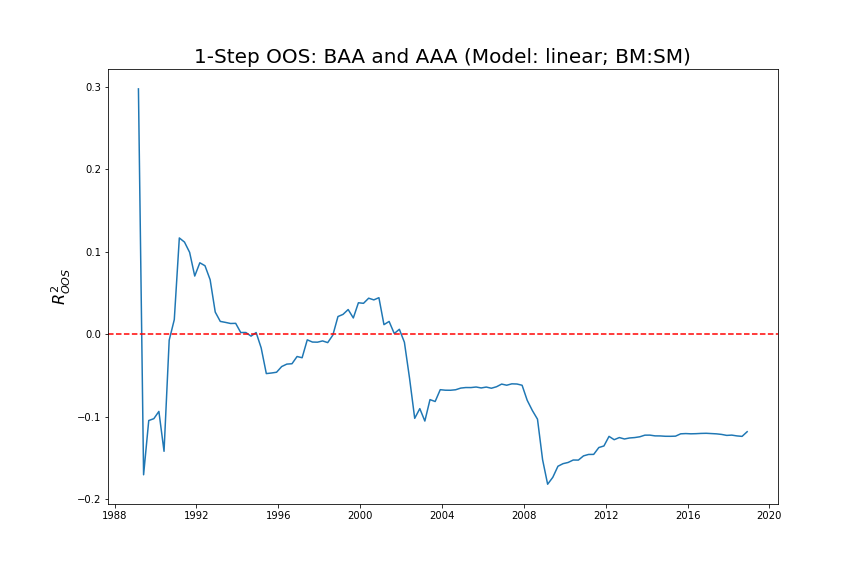
\includegraphics[width=0.9\linewidth]{OOS_plots/linear_co4_SM.png}
			\caption{co4}
		\end{subfigure}
		\label{g8}
	\end{figure}
	\pagebreak
	
	To compare the performances of the 8 functional forms with the 4 different variable combinations, we calculate the percentage of positive $R^2_{OOS}$ in the forecasting period. The results are shown in table (\ref{perct}). It is clear that for combination co3 (dp and ep), none of the functions can perform better than sample mean prediction. However, for combinations co2 and co4, for more than half of out-of-sample period, $g_1$ and $g_6$ can outperform sample mean. And other functional forms also can provide positive results. 
	
	% Table generated by Excel2LaTeX from sheet 'Sheet1'
	\begin{table}[htbp]
		\centering
		\caption{Percentage of Positive $R^2_{OOS}$}
		\begin{tabular}{ccccccccc}
			\toprule
			& $g_1$    & $g_2$    & $g_3$    & $g_4$    & $g_5$    & $g_6$    & $g_7$    & $g_8$ \\
			\midrule
			co1   & 3.23\% & 3.23\% & 0.00\% & 0.00\% & 2.42\% & 7.26\% & 4.03\% & 0.00\% \\
			co2   & 37.90\% & 37.90\% & 32.26\% & 32.26\% & 2.42\% & \textcolor[rgb]{ .753,  0,  0}{68.55\%} & 29.84\% & 32.26\% \\
			co3   & 0.00\% & 0.00\% & 0.00\% & 0.00\% & 0.00\% & 0.00\% & 0.00\% & 0.00\% \\
			co4   & \textcolor[rgb]{ .753,  0,  0}{57.26\%} & 24.19\% & 24.19\% & 26.61\% & 2.42\% & \textcolor[rgb]{ .753,  0,  0}{62.90\%} & 41.94\% & 27.42\% \\
			\bottomrule
			\bottomrule
		\end{tabular}%
		\label{perct}%
	\end{table}%
	
	To conclude, no matter which function we use, combinations co2 and co4 tend to have better results than other variable pairs. And among the 8 functions, $g_6$ is the best for all the 4 combinations in terms of the percentage of positive $R^2_{OOS}$. The two trigonometric functions also provide good OOS results, especially for $g_1$ and co4. But considering the scale parameter in $g_3$ and $g_4$ does not improve the forecast. For polynomial function, it can outperform sample mean except for combination co3, although it is not as good as other functional forms.
	
	\section{conclusion}
	In this chapter, we consider a partially nonlinear single-index model, which allows for lagged dependent variables, stationary variables, cointegrated and non-cointegrated variables. We propose a two-step estimation method to estimate the model and includes a constraint on $\theta$ (the coefficient for the non-stationary variables). From the simulation results, we can see that the estimators have good finite sample properties and the constraint provides finite sample gains. 
	
	We apply the model to the \cite{welch2008comprehensive} dataset and investigate the predictability using co-integrated variable combinations. We find that by including lagged dependent variable and stationary variable, the partially nonlinear single-index models obtain a better out-of-sample performance than the nonlinear models. When using the partially nonlinear model, some of the variable combinations in previous studies give better out-of-sample forecast than the sample mean prediction over a consecutive period. 
	
	\chapter*{Timetable}
	\addcontentsline{toc}{chapter}{Timetable}
	\subsection*{Timetable for 2020}
	After my confirmation report, I followed the research schedule proposed for chapter 2 and finished the Monte Carlo simulation and empirical study.
	
	\begin{itemize}
		\item April 2020 - Jul 2020: Extended the simulation I have done in first year.
		
		In my confirmation report, I considered three functional forms (two trigonometric functions and one polynomial function) and two cases (stationary and noncointegrated predictors). 
		
		I then included 2 exponential functions and also considered cointegrated predictor case in the simulation. 
		
		\item Aug 2020 - mid Dec 2020: I finished the empirical study using the five nonlinear functions and find that they can provide a better performance than the benchmark model. 
		
		\item Nov - Dec I started to write chapter 2.
		
		\item Jan 2020 - Feb 2021: Started to extend the nonstationary nonlinear single-index model to a partially nonlinear single-index model. Introduced a new estimation method for the model in chapter 3.
	\end{itemize}
	
	\subsection*{Timetable for 2021}
	In the coming year of my PhD program, I am going to keep working on chapter 3 - the partially nonlinear single-index model. Here is my timetable:
	
	\begin{itemize}
		\item Mar 2021 - Jul 2021:  I will conduct simulation experiment for chapter 3 and  compare the finite sample properties of NLS and CLS estimator under different cases (noncointegrated, cointegrated, serially correlated error.)
		
		\item Aug 2021 - Nov 2021: I will conduct the empirical study to illustrate the usefulness of the partially nonlinear single-index model. Then I will write chapter 3.
		
		\item Nov 2021 - Feb 2022: I will establish the asymptotic properties of the estimators.
	\end{itemize}
	
	
	%I will first enrich the literature review for the new chapter. Then, I will use Monte Carlo simulation method to investigate and compare the finite sample properties of the NLS estimators and CLS estimators. Following the study of \cite{zhou2018semiparametric}, we will also consider VMA and VARMA error structure in data generation processes:
	
	%\begin{enumerate}
	%	
	%	\item VMA structure in data generation process:
	%	
	%	$$x_t = x_{t-1} + v_t$$
	%	$$v_t = \epsilon_t + C_{10}*\epsilon_{t-1}$$
	%	where $\epsilon_{t} \sim i i N\left(0,\left(\begin{array}{cc}1 & 0.5 \\ 0.5 & 1\end{array}\right)\right)$,  $C_{10}=\left(\begin{array}{cc} -1  & 4/ 3 \\ 0 & 0\end{array}\right)$. 
	%	
	%	\item VARMA structure in data generation process:
	%	$$x_t = x_{t-1} + v_t$$
	%	$$v_t = A_0 v_{2t-1} + \epsilon_t + C_{20}*\epsilon_{t-1}$$
	%	where $\epsilon_{t} \sim i i N\left(0,\left(\begin{array}{cc}1 & 0.5 \\ 0.5 & 1\end{array}\right)\right)$, $A_{0}=\left(\begin{array}{cc} 2/5  & 0 \\ 0 & 0\end{array}\right)$, $C_{20}=\left(\begin{array}{cc} -1  & 5/4 \\ 0 & 0\end{array}\right)$. 
	%\end{enumerate}
	%
	%We expect that under both of the above data generation processes, the estimators will have a satisfactory finite sample performance. Moreover, since the constrain acts as an identification condition, we expect that the finite sample performances of $\theta_{1}$ and $\theta_{2}$ will improved. 
	%
	%In the empirical analysis, we will apply the partially nonlinear single-index model to the \cite{welch2008comprehensive} dataset to study stock return predictability. As for the cointegrated variables, we will refer to the study \cite{zhou2018semiparametric} and \cite{lettau2001consumption}. Since we have included the lagged dependent variable $y_{t-1}$ in the partially nonlinear model, we expect that the OOS forecasting results can be improved compared with previous chapter, where $y_{t-1}$ and other stationary variables have not been included.
	
	%Many financial ratios were found to be useful in predicting stork return. But the predictability has then been challenged due to the persistence in these predictors and the unbalance issue from linear predictive models. To address these econometric problems, our paper adopts a multivariate parametric single-index predictive model. The parameters in this model can be estimated by nonlinear least square method, but we contribute by imposing truncation and identification constrains, which significantly improves the finite sample properties of the estimators. Another important contribution of this paper is that, our paper unveils the single-index model’s ability in predicting stock return. We demonstrate that some predictors, especially co-integrated predictors, such as yields of BAA and AAA rated bonds, provide a better performance than the historical average in a consecutive period. 
	\bigskip
	
	{\footnotesize
		
		\bibliographystyle{agsm}
		\bibliography{reference}
		
	}
	
	
	{\small
		\renewcommand{\thetable}{\Alph{section}\arabic{table}}
		\renewcommand{\thefigure}{\Alph{section}\arabic{figure}}
		\setcounter{figure}{0}
		\setcounter{table}{0}
		
		%\appendix
		%\section{Discussion on the assumptions}\label{appendix_a}
		
		
		%{\footnotesize
		%\bibliographystyle{chicago}
		%\bibliographystyle{apalike}
		%\bibliography{reference}
	}
	
	
	
	
	
\end{document} 